\documentclass[a4paper]{book}
\usepackage{makeidx}
\usepackage{graphicx}
\usepackage{multicol}
\usepackage{float}
\usepackage{listings}
\usepackage{color}
\usepackage{ifthen}
\usepackage[table]{xcolor}
\usepackage{textcomp}
\usepackage{alltt}
\usepackage{ifpdf}
\ifpdf
\usepackage[pdftex,
            pagebackref=true,
            colorlinks=true,
            linkcolor=blue,
            unicode
           ]{hyperref}
\else
\usepackage[ps2pdf,
            pagebackref=true,
            colorlinks=true,
            linkcolor=blue,
            unicode
           ]{hyperref}
\usepackage{pspicture}
\fi
\usepackage[utf8]{inputenc}
\usepackage{mathptmx}
\usepackage[scaled=.90]{helvet}
\usepackage{courier}
\usepackage{sectsty}
\usepackage[titles]{tocloft}
\usepackage{doxygen}
\lstset{language=C++,inputencoding=utf8,basicstyle=\footnotesize,breaklines=true,breakatwhitespace=true,tabsize=8,numbers=left }
\makeindex
\setcounter{tocdepth}{3}
\renewcommand{\footrulewidth}{0.4pt}
\renewcommand{\familydefault}{\sfdefault}
\begin{document}
\hypersetup{pageanchor=false}
\begin{titlepage}
\vspace*{7cm}
\begin{center}
{\Large MalELFicus }\\
\vspace*{1cm}
{\large Generated by Doxygen 1.7.4}\\
\vspace*{0.5cm}
{\small Sat Nov 3 2012 18:49:10}\\
\end{center}
\end{titlepage}
\clearemptydoublepage
\pagenumbering{roman}
\tableofcontents
\clearemptydoublepage
\pagenumbering{arabic}
\hypersetup{pageanchor=true}
\chapter{Malelficus ELF Library}
\label{index}\hypertarget{index}{}\begin{DoxyAuthor}{Authors}
i4k
\end{DoxyAuthor}
\hypertarget{index_Introduction}{}\section{Introduction}\label{index_Introduction}
LibMalelf is part of MalELFicus toolkit. The library can be used for analysis of ELF binaries for malware or reverse engineering.


\begin{DoxyItemize}
\item Implementation files
\end{DoxyItemize}
\begin{DoxyEnumerate}
\item templates/ClassTemplate.h
\item src/ClassTemplate.cxx
\end{DoxyEnumerate}
\begin{DoxyItemize}
\item User-\/Defined Gaudi Algorithm
\end{DoxyItemize}
\begin{DoxyEnumerate}
\item src/ExampleAlg.cxx
\item src/Dll/templates\_\-dll.cxx
\item src/Dll/templates\_\-load.cxx
\end{DoxyEnumerate}
\begin{DoxyItemize}
\item User-\/Defined Gaudi Service
\end{DoxyItemize}
\begin{DoxyEnumerate}
\item templates/IExampleSvc.h
\item templates/ExampleSvc.h
\item src/ExampleSvc.cxx
\item src/Dll/templates\_\-dll.cxx
\item src/Dll/templates\_\-load.cxx
\end{DoxyEnumerate}

Also note the existence of the following directories:
\begin{DoxyItemize}
\item cmt
\end{DoxyItemize}
\begin{DoxyEnumerate}
\item Contains the requirements file
\end{DoxyEnumerate}
\begin{DoxyItemize}
\item doc
\end{DoxyItemize}
\begin{DoxyEnumerate}
\item Contains the release.notes file
\end{DoxyEnumerate}

As you prepare to develop code for GLAST SAS, please be sure you are aware of our current \href{http://www-glast.slac.stanford.edu/software/CodeHowTo/codeStandards.html}{\tt Coding Standards }

If using the code in this package as an example -\/ please modify the comments as appropriate for your own specific code.



 \hypertarget{index_notes}{}\section{release.notes}\label{index_notes}
release.notes 

 \hypertarget{index_requirements}{}\section{requirements}\label{index_requirements}

\begin{DoxyVerbInclude}
\end{DoxyVerbInclude}
 

 \begin{Desc}
\item[\hyperlink{todo__todo000001}{Todo}]\mbox{[}optionally include text about more work to be done\mbox{]} 

Give each todo item its own line\end{Desc}

\chapter{Todo List}
\label{todo}
\hypertarget{todo}{}
\label{todo__todo000001}
\hypertarget{todo__todo000001}{}
 
\begin{DoxyDescription}
\item[page \hyperlink{index}{Malelficus ELF Library} ]\mbox{[}optionally include text about more work to be done\mbox{]} 

Give each todo item its own line
\end{DoxyDescription}
\chapter{Class Index}
\section{Class List}
Here are the classes, structs, unions and interfaces with brief descriptions:\begin{DoxyCompactList}
\item\contentsline{section}{\hyperlink{structmalelf__add__section__t}{malelf\_\-add\_\-section\_\-t} }{\pageref{structmalelf__add__section__t}}{}
\item\contentsline{section}{\hyperlink{structmalelf__dissect__opt}{malelf\_\-dissect\_\-opt} }{\pageref{structmalelf__dissect__opt}}{}
\item\contentsline{section}{\hyperlink{unionmalelf__dword}{malelf\_\-dword} }{\pageref{unionmalelf__dword}}{}
\item\contentsline{section}{\hyperlink{structmalelf__elf__attr}{malelf\_\-elf\_\-attr} }{\pageref{structmalelf__elf__attr}}{}
\item\contentsline{section}{\hyperlink{structmalelf__elf__t}{malelf\_\-elf\_\-t} }{\pageref{structmalelf__elf__t}}{}
\item\contentsline{section}{\hyperlink{structmalelf__object}{malelf\_\-object} }{\pageref{structmalelf__object}}{}
\item\contentsline{section}{\hyperlink{structtb__column}{tb\_\-column} }{\pageref{structtb__column}}{}
\item\contentsline{section}{\hyperlink{structtb__line}{tb\_\-line} }{\pageref{structtb__line}}{}
\end{DoxyCompactList}

\chapter{File Index}
\section{File List}
Here is a list of all files with brief descriptions:\begin{DoxyCompactList}
\item\contentsline{section}{src/libmalelf/\hyperlink{copy_8c}{copy.c} }{\pageref{copy_8c}}{}
\item\contentsline{section}{src/libmalelf/\hyperlink{disas_8c}{disas.c} }{\pageref{disas_8c}}{}
\item\contentsline{section}{src/libmalelf/\hyperlink{dissect_8c}{dissect.c} }{\pageref{dissect_8c}}{}
\item\contentsline{section}{src/libmalelf/\hyperlink{error_8c}{error.c} }{\pageref{error_8c}}{}
\item\contentsline{section}{src/libmalelf/\hyperlink{header__types_8inc}{header\_\-types.inc} }{\pageref{header__types_8inc}}{}
\item\contentsline{section}{src/libmalelf/\hyperlink{infect_8c}{infect.c} }{\pageref{infect_8c}}{}
\item\contentsline{section}{src/libmalelf/\hyperlink{machines_8inc}{machines.inc} }{\pageref{machines_8inc}}{}
\item\contentsline{section}{src/libmalelf/\hyperlink{mainpage_8h}{mainpage.h} (Definition of class Template )}{\pageref{mainpage_8h}}{}
\item\contentsline{section}{src/libmalelf/\hyperlink{object_8c}{object.c} }{\pageref{object_8c}}{}
\item\contentsline{section}{src/libmalelf/\hyperlink{print__table_8c}{print\_\-table.c} }{\pageref{print__table_8c}}{}
\item\contentsline{section}{src/libmalelf/\hyperlink{reverse__elf_8c}{reverse\_\-elf.c} }{\pageref{reverse__elf_8c}}{}
\item\contentsline{section}{src/libmalelf/\hyperlink{section__types_8inc}{section\_\-types.inc} }{\pageref{section__types_8inc}}{}
\item\contentsline{section}{src/libmalelf/\hyperlink{segment__flags_8inc}{segment\_\-flags.inc} }{\pageref{segment__flags_8inc}}{}
\item\contentsline{section}{src/libmalelf/\hyperlink{segment__types_8inc}{segment\_\-types.inc} }{\pageref{segment__types_8inc}}{}
\item\contentsline{section}{src/libmalelf/\hyperlink{shellcode_8c}{shellcode.c} }{\pageref{shellcode_8c}}{}
\item\contentsline{section}{src/libmalelf/\hyperlink{util_8c}{util.c} }{\pageref{util_8c}}{}
\item\contentsline{section}{src/libmalelf/include/malelf/\hyperlink{defines_8h}{defines.h} }{\pageref{defines_8h}}{}
\item\contentsline{section}{src/libmalelf/include/malelf/\hyperlink{disas_8h}{disas.h} }{\pageref{disas_8h}}{}
\item\contentsline{section}{src/libmalelf/include/malelf/\hyperlink{dissect_8h}{dissect.h} }{\pageref{dissect_8h}}{}
\item\contentsline{section}{src/libmalelf/include/malelf/\hyperlink{error_8h}{error.h} }{\pageref{error_8h}}{}
\item\contentsline{section}{src/libmalelf/include/malelf/\hyperlink{infect_8h}{infect.h} }{\pageref{infect_8h}}{}
\item\contentsline{section}{src/libmalelf/include/malelf/\hyperlink{malelf_8h}{malelf.h} }{\pageref{malelf_8h}}{}
\item\contentsline{section}{src/libmalelf/include/malelf/\hyperlink{object_8h}{object.h} }{\pageref{object_8h}}{}
\item\contentsline{section}{src/libmalelf/include/malelf/\hyperlink{print__table_8h}{print\_\-table.h} }{\pageref{print__table_8h}}{}
\item\contentsline{section}{src/libmalelf/include/malelf/\hyperlink{reverse__elf_8h}{reverse\_\-elf.h} }{\pageref{reverse__elf_8h}}{}
\item\contentsline{section}{src/libmalelf/include/malelf/\hyperlink{shellcode_8h}{shellcode.h} }{\pageref{shellcode_8h}}{}
\item\contentsline{section}{src/libmalelf/include/malelf/\hyperlink{types_8h}{types.h} }{\pageref{types_8h}}{}
\item\contentsline{section}{src/libmalelf/include/malelf/\hyperlink{util_8h}{util.h} }{\pageref{util_8h}}{}
\end{DoxyCompactList}

\chapter{Class Documentation}
\hypertarget{structmalelf__add__section__t}{
\section{malelf\_\-add\_\-section\_\-t Struct Reference}
\label{structmalelf__add__section__t}\index{malelf\_\-add\_\-section\_\-t@{malelf\_\-add\_\-section\_\-t}}
}


{\ttfamily \#include $<$object.h$>$}

\subsection*{Public Attributes}
\begin{DoxyCompactItemize}
\item 
const char $\ast$ \hyperlink{structmalelf__add__section__t_a6f46f282d559886a9626822f1a073428}{name}
\item 
const char $\ast$ \hyperlink{structmalelf__add__section__t_a094c67dd6768305395085f96549def2f}{data\_\-fname}
\end{DoxyCompactItemize}


\subsection{Detailed Description}


Definition at line 56 of file object.h.



\subsection{Member Data Documentation}
\hypertarget{structmalelf__add__section__t_a094c67dd6768305395085f96549def2f}{
\index{malelf\_\-add\_\-section\_\-t@{malelf\_\-add\_\-section\_\-t}!data\_\-fname@{data\_\-fname}}
\index{data\_\-fname@{data\_\-fname}!malelf_add_section_t@{malelf\_\-add\_\-section\_\-t}}
\subsubsection[{data\_\-fname}]{\setlength{\rightskip}{0pt plus 5cm}const char$\ast$ {\bf malelf\_\-add\_\-section\_\-t::data\_\-fname}}}
\label{structmalelf__add__section__t_a094c67dd6768305395085f96549def2f}


Definition at line 58 of file object.h.

\hypertarget{structmalelf__add__section__t_a6f46f282d559886a9626822f1a073428}{
\index{malelf\_\-add\_\-section\_\-t@{malelf\_\-add\_\-section\_\-t}!name@{name}}
\index{name@{name}!malelf_add_section_t@{malelf\_\-add\_\-section\_\-t}}
\subsubsection[{name}]{\setlength{\rightskip}{0pt plus 5cm}const char$\ast$ {\bf malelf\_\-add\_\-section\_\-t::name}}}
\label{structmalelf__add__section__t_a6f46f282d559886a9626822f1a073428}


Definition at line 57 of file object.h.



The documentation for this struct was generated from the following file:\begin{DoxyCompactItemize}
\item 
src/libmalelf/include/malelf/\hyperlink{object_8h}{object.h}\end{DoxyCompactItemize}

\hypertarget{structmalelf__dissect__opt}{
\section{malelf\_\-dissect\_\-opt Struct Reference}
\label{structmalelf__dissect__opt}\index{malelf\_\-dissect\_\-opt@{malelf\_\-dissect\_\-opt}}
}


{\ttfamily \#include $<$types.h$>$}

\subsection*{Public Attributes}
\begin{DoxyCompactItemize}
\item 
\hyperlink{types_8h_af2b0f13cffd24f6dddf794ae0c7472b4}{\_\-u8} \hyperlink{structmalelf__dissect__opt_aa6ceee630d61c83113d6f0469646880a}{is\_\-header}
\item 
\hyperlink{types_8h_af2b0f13cffd24f6dddf794ae0c7472b4}{\_\-u8} \hyperlink{structmalelf__dissect__opt_a6d7284ba8a221d54022192ac572a8244}{is\_\-pht}
\item 
\hyperlink{types_8h_af2b0f13cffd24f6dddf794ae0c7472b4}{\_\-u8} \hyperlink{structmalelf__dissect__opt_a9a8942b6b82bc1baac39701bc722f96d}{is\_\-sht}
\end{DoxyCompactItemize}


\subsection{Detailed Description}


Definition at line 14 of file types.h.



\subsection{Member Data Documentation}
\hypertarget{structmalelf__dissect__opt_aa6ceee630d61c83113d6f0469646880a}{
\index{malelf\_\-dissect\_\-opt@{malelf\_\-dissect\_\-opt}!is\_\-header@{is\_\-header}}
\index{is\_\-header@{is\_\-header}!malelf_dissect_opt@{malelf\_\-dissect\_\-opt}}
\subsubsection[{is\_\-header}]{\setlength{\rightskip}{0pt plus 5cm}{\bf \_\-u8} {\bf malelf\_\-dissect\_\-opt::is\_\-header}}}
\label{structmalelf__dissect__opt_aa6ceee630d61c83113d6f0469646880a}


Definition at line 15 of file types.h.

\hypertarget{structmalelf__dissect__opt_a6d7284ba8a221d54022192ac572a8244}{
\index{malelf\_\-dissect\_\-opt@{malelf\_\-dissect\_\-opt}!is\_\-pht@{is\_\-pht}}
\index{is\_\-pht@{is\_\-pht}!malelf_dissect_opt@{malelf\_\-dissect\_\-opt}}
\subsubsection[{is\_\-pht}]{\setlength{\rightskip}{0pt plus 5cm}{\bf \_\-u8} {\bf malelf\_\-dissect\_\-opt::is\_\-pht}}}
\label{structmalelf__dissect__opt_a6d7284ba8a221d54022192ac572a8244}


Definition at line 16 of file types.h.

\hypertarget{structmalelf__dissect__opt_a9a8942b6b82bc1baac39701bc722f96d}{
\index{malelf\_\-dissect\_\-opt@{malelf\_\-dissect\_\-opt}!is\_\-sht@{is\_\-sht}}
\index{is\_\-sht@{is\_\-sht}!malelf_dissect_opt@{malelf\_\-dissect\_\-opt}}
\subsubsection[{is\_\-sht}]{\setlength{\rightskip}{0pt plus 5cm}{\bf \_\-u8} {\bf malelf\_\-dissect\_\-opt::is\_\-sht}}}
\label{structmalelf__dissect__opt_a9a8942b6b82bc1baac39701bc722f96d}


Definition at line 17 of file types.h.



The documentation for this struct was generated from the following file:\begin{DoxyCompactItemize}
\item 
src/libmalelf/include/malelf/\hyperlink{types_8h}{types.h}\end{DoxyCompactItemize}

\hypertarget{unionmalelf__dword}{
\section{malelf\_\-dword Union Reference}
\label{unionmalelf__dword}\index{malelf\_\-dword@{malelf\_\-dword}}
}


{\ttfamily \#include $<$object.h$>$}

\subsection*{Public Attributes}
\begin{DoxyCompactItemize}
\item 
unsigned long int \hyperlink{unionmalelf__dword_a22dbf267cecf05067febc84ac0645775}{long\_\-val}
\item 
unsigned char \hyperlink{unionmalelf__dword_a1f65f347531fda3fbcb41779fa674701}{char\_\-val} \mbox{[}4\mbox{]}
\end{DoxyCompactItemize}


\subsection{Detailed Description}


Definition at line 29 of file object.h.



\subsection{Member Data Documentation}
\hypertarget{unionmalelf__dword_a1f65f347531fda3fbcb41779fa674701}{
\index{malelf\_\-dword@{malelf\_\-dword}!char\_\-val@{char\_\-val}}
\index{char\_\-val@{char\_\-val}!malelf_dword@{malelf\_\-dword}}
\subsubsection[{char\_\-val}]{\setlength{\rightskip}{0pt plus 5cm}unsigned char {\bf malelf\_\-dword::char\_\-val}\mbox{[}4\mbox{]}}}
\label{unionmalelf__dword_a1f65f347531fda3fbcb41779fa674701}


Definition at line 31 of file object.h.

\hypertarget{unionmalelf__dword_a22dbf267cecf05067febc84ac0645775}{
\index{malelf\_\-dword@{malelf\_\-dword}!long\_\-val@{long\_\-val}}
\index{long\_\-val@{long\_\-val}!malelf_dword@{malelf\_\-dword}}
\subsubsection[{long\_\-val}]{\setlength{\rightskip}{0pt plus 5cm}unsigned long int {\bf malelf\_\-dword::long\_\-val}}}
\label{unionmalelf__dword_a22dbf267cecf05067febc84ac0645775}


Definition at line 30 of file object.h.



The documentation for this union was generated from the following file:\begin{DoxyCompactItemize}
\item 
src/libmalelf/include/malelf/\hyperlink{object_8h}{object.h}\end{DoxyCompactItemize}

\hypertarget{structmalelf__elf__attr}{
\section{malelf\_\-elf\_\-attr Struct Reference}
\label{structmalelf__elf__attr}\index{malelf\_\-elf\_\-attr@{malelf\_\-elf\_\-attr}}
}


{\ttfamily \#include $<$object.h$>$}

\subsection*{Public Attributes}
\begin{DoxyCompactItemize}
\item 
char $\ast$ \hyperlink{structmalelf__elf__attr_a94413655d886dc859f66668fbf04be95}{name}
\item 
\hyperlink{types_8h_a07491c35a48354e0e7b56974a04cc3de}{\_\-u32} \hyperlink{structmalelf__elf__attr_af49e74a88d3f8f78a0ab58ba788afcbc}{val}
\item 
char $\ast$ \hyperlink{structmalelf__elf__attr_a04fe708024668b47fbc67edb611c3e45}{desc}
\end{DoxyCompactItemize}


\subsection{Detailed Description}


Definition at line 50 of file object.h.



\subsection{Member Data Documentation}
\hypertarget{structmalelf__elf__attr_a04fe708024668b47fbc67edb611c3e45}{
\index{malelf\_\-elf\_\-attr@{malelf\_\-elf\_\-attr}!desc@{desc}}
\index{desc@{desc}!malelf_elf_attr@{malelf\_\-elf\_\-attr}}
\subsubsection[{desc}]{\setlength{\rightskip}{0pt plus 5cm}char$\ast$ {\bf malelf\_\-elf\_\-attr::desc}}}
\label{structmalelf__elf__attr_a04fe708024668b47fbc67edb611c3e45}


Definition at line 53 of file object.h.

\hypertarget{structmalelf__elf__attr_a94413655d886dc859f66668fbf04be95}{
\index{malelf\_\-elf\_\-attr@{malelf\_\-elf\_\-attr}!name@{name}}
\index{name@{name}!malelf_elf_attr@{malelf\_\-elf\_\-attr}}
\subsubsection[{name}]{\setlength{\rightskip}{0pt plus 5cm}char$\ast$ {\bf malelf\_\-elf\_\-attr::name}}}
\label{structmalelf__elf__attr_a94413655d886dc859f66668fbf04be95}


Definition at line 51 of file object.h.

\hypertarget{structmalelf__elf__attr_af49e74a88d3f8f78a0ab58ba788afcbc}{
\index{malelf\_\-elf\_\-attr@{malelf\_\-elf\_\-attr}!val@{val}}
\index{val@{val}!malelf_elf_attr@{malelf\_\-elf\_\-attr}}
\subsubsection[{val}]{\setlength{\rightskip}{0pt plus 5cm}{\bf \_\-u32} {\bf malelf\_\-elf\_\-attr::val}}}
\label{structmalelf__elf__attr_af49e74a88d3f8f78a0ab58ba788afcbc}


Definition at line 52 of file object.h.



The documentation for this struct was generated from the following file:\begin{DoxyCompactItemize}
\item 
src/libmalelf/include/malelf/\hyperlink{object_8h}{object.h}\end{DoxyCompactItemize}

\hypertarget{structmalelf__elf__t}{
\section{malelf\_\-elf\_\-t Struct Reference}
\label{structmalelf__elf__t}\index{malelf\_\-elf\_\-t@{malelf\_\-elf\_\-t}}
}


{\ttfamily \#include $<$object.h$>$}

\subsection*{Public Member Functions}
\begin{DoxyCompactItemize}
\item 
\hyperlink{structmalelf__elf__t_a3a2fcb24f1cc3aec9b6656953c391b2e}{ElfW} (Ehdr)$\ast$elfh
\item 
\hyperlink{structmalelf__elf__t_ad39aff9abba5f6394ccd48eca6cc02e3}{ElfW} (Phdr)$\ast$elfp
\item 
\hyperlink{structmalelf__elf__t_ab13051d50f844e065267c53816be9b08}{ElfW} (Shdr)$\ast$elfs
\end{DoxyCompactItemize}


\subsection{Detailed Description}


Definition at line 34 of file object.h.



\subsection{Member Function Documentation}
\hypertarget{structmalelf__elf__t_a3a2fcb24f1cc3aec9b6656953c391b2e}{
\index{malelf\_\-elf\_\-t@{malelf\_\-elf\_\-t}!ElfW@{ElfW}}
\index{ElfW@{ElfW}!malelf_elf_t@{malelf\_\-elf\_\-t}}
\subsubsection[{ElfW}]{\setlength{\rightskip}{0pt plus 5cm}malelf\_\-elf\_\-t::ElfW (
\begin{DoxyParamCaption}
\item[{Ehdr}]{}
\end{DoxyParamCaption}
)}}
\label{structmalelf__elf__t_a3a2fcb24f1cc3aec9b6656953c391b2e}
\hypertarget{structmalelf__elf__t_ab13051d50f844e065267c53816be9b08}{
\index{malelf\_\-elf\_\-t@{malelf\_\-elf\_\-t}!ElfW@{ElfW}}
\index{ElfW@{ElfW}!malelf_elf_t@{malelf\_\-elf\_\-t}}
\subsubsection[{ElfW}]{\setlength{\rightskip}{0pt plus 5cm}malelf\_\-elf\_\-t::ElfW (
\begin{DoxyParamCaption}
\item[{Shdr}]{}
\end{DoxyParamCaption}
)}}
\label{structmalelf__elf__t_ab13051d50f844e065267c53816be9b08}
\hypertarget{structmalelf__elf__t_ad39aff9abba5f6394ccd48eca6cc02e3}{
\index{malelf\_\-elf\_\-t@{malelf\_\-elf\_\-t}!ElfW@{ElfW}}
\index{ElfW@{ElfW}!malelf_elf_t@{malelf\_\-elf\_\-t}}
\subsubsection[{ElfW}]{\setlength{\rightskip}{0pt plus 5cm}malelf\_\-elf\_\-t::ElfW (
\begin{DoxyParamCaption}
\item[{Phdr}]{}
\end{DoxyParamCaption}
)}}
\label{structmalelf__elf__t_ad39aff9abba5f6394ccd48eca6cc02e3}


The documentation for this struct was generated from the following file:\begin{DoxyCompactItemize}
\item 
src/libmalelf/include/malelf/\hyperlink{object_8h}{object.h}\end{DoxyCompactItemize}

\hypertarget{structmalelf__object}{
\section{malelf\_\-object Struct Reference}
\label{structmalelf__object}\index{malelf\_\-object@{malelf\_\-object}}
}


{\ttfamily \#include $<$object.h$>$}



Collaboration diagram for malelf\_\-object:\nopagebreak
\begin{figure}[H]
\begin{center}
\leavevmode
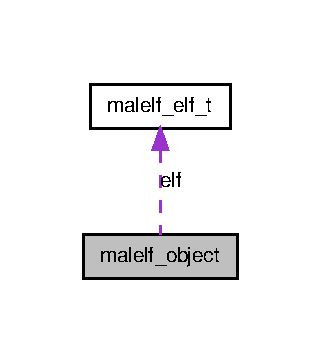
\includegraphics[width=154pt]{structmalelf__object__coll__graph}
\end{center}
\end{figure}
\subsection*{Public Attributes}
\begin{DoxyCompactItemize}
\item 
char $\ast$ \hyperlink{structmalelf__object_a726458fb460f6a24831c86c8b38c0266}{fname}
\item 
int \hyperlink{structmalelf__object_ae97de1bc2fbeea9832e6a967953d2446}{fd}
\item 
struct stat \hyperlink{structmalelf__object_a33c04ec75fc3c04fb71c4df805338a40}{st\_\-info}
\item 
\hyperlink{types_8h_af2b0f13cffd24f6dddf794ae0c7472b4}{\_\-u8} $\ast$ \hyperlink{structmalelf__object_a8a910606f6b5bf327ba116b89b017887}{mem}
\item 
\hyperlink{structmalelf__elf__t}{malelf\_\-elf\_\-t} \hyperlink{structmalelf__object_aaed8855ad6d68c50f72ec6a9d61dcefb}{elf}
\item 
\hyperlink{types_8h_af2b0f13cffd24f6dddf794ae0c7472b4}{\_\-u8} \hyperlink{structmalelf__object_a3032145296090f7b882d44756596a18c}{is\_\-readonly}
\item 
\hyperlink{object_8h_a24f8376c4f2e7c8f8c023d1733ab02e9}{alloc\_\-type\_\-t} \hyperlink{structmalelf__object_a458bc33779f59e8534c7529cd6791043}{alloc\_\-type}
\end{DoxyCompactItemize}


\subsection{Detailed Description}


Definition at line 40 of file object.h.



\subsection{Member Data Documentation}
\hypertarget{structmalelf__object_a458bc33779f59e8534c7529cd6791043}{
\index{malelf\_\-object@{malelf\_\-object}!alloc\_\-type@{alloc\_\-type}}
\index{alloc\_\-type@{alloc\_\-type}!malelf_object@{malelf\_\-object}}
\subsubsection[{alloc\_\-type}]{\setlength{\rightskip}{0pt plus 5cm}{\bf alloc\_\-type\_\-t} {\bf malelf\_\-object::alloc\_\-type}}}
\label{structmalelf__object_a458bc33779f59e8534c7529cd6791043}


Definition at line 47 of file object.h.

\hypertarget{structmalelf__object_aaed8855ad6d68c50f72ec6a9d61dcefb}{
\index{malelf\_\-object@{malelf\_\-object}!elf@{elf}}
\index{elf@{elf}!malelf_object@{malelf\_\-object}}
\subsubsection[{elf}]{\setlength{\rightskip}{0pt plus 5cm}{\bf malelf\_\-elf\_\-t} {\bf malelf\_\-object::elf}}}
\label{structmalelf__object_aaed8855ad6d68c50f72ec6a9d61dcefb}


Definition at line 45 of file object.h.

\hypertarget{structmalelf__object_ae97de1bc2fbeea9832e6a967953d2446}{
\index{malelf\_\-object@{malelf\_\-object}!fd@{fd}}
\index{fd@{fd}!malelf_object@{malelf\_\-object}}
\subsubsection[{fd}]{\setlength{\rightskip}{0pt plus 5cm}int {\bf malelf\_\-object::fd}}}
\label{structmalelf__object_ae97de1bc2fbeea9832e6a967953d2446}


Definition at line 42 of file object.h.

\hypertarget{structmalelf__object_a726458fb460f6a24831c86c8b38c0266}{
\index{malelf\_\-object@{malelf\_\-object}!fname@{fname}}
\index{fname@{fname}!malelf_object@{malelf\_\-object}}
\subsubsection[{fname}]{\setlength{\rightskip}{0pt plus 5cm}char$\ast$ {\bf malelf\_\-object::fname}}}
\label{structmalelf__object_a726458fb460f6a24831c86c8b38c0266}


Definition at line 41 of file object.h.

\hypertarget{structmalelf__object_a3032145296090f7b882d44756596a18c}{
\index{malelf\_\-object@{malelf\_\-object}!is\_\-readonly@{is\_\-readonly}}
\index{is\_\-readonly@{is\_\-readonly}!malelf_object@{malelf\_\-object}}
\subsubsection[{is\_\-readonly}]{\setlength{\rightskip}{0pt plus 5cm}{\bf \_\-u8} {\bf malelf\_\-object::is\_\-readonly}}}
\label{structmalelf__object_a3032145296090f7b882d44756596a18c}


Definition at line 46 of file object.h.

\hypertarget{structmalelf__object_a8a910606f6b5bf327ba116b89b017887}{
\index{malelf\_\-object@{malelf\_\-object}!mem@{mem}}
\index{mem@{mem}!malelf_object@{malelf\_\-object}}
\subsubsection[{mem}]{\setlength{\rightskip}{0pt plus 5cm}{\bf \_\-u8}$\ast$ {\bf malelf\_\-object::mem}}}
\label{structmalelf__object_a8a910606f6b5bf327ba116b89b017887}


Definition at line 44 of file object.h.

\hypertarget{structmalelf__object_a33c04ec75fc3c04fb71c4df805338a40}{
\index{malelf\_\-object@{malelf\_\-object}!st\_\-info@{st\_\-info}}
\index{st\_\-info@{st\_\-info}!malelf_object@{malelf\_\-object}}
\subsubsection[{st\_\-info}]{\setlength{\rightskip}{0pt plus 5cm}struct stat {\bf malelf\_\-object::st\_\-info}}}
\label{structmalelf__object_a33c04ec75fc3c04fb71c4df805338a40}


Definition at line 43 of file object.h.



The documentation for this struct was generated from the following file:\begin{DoxyCompactItemize}
\item 
src/libmalelf/include/malelf/\hyperlink{object_8h}{object.h}\end{DoxyCompactItemize}

\hypertarget{structtb__column}{
\section{tb\_\-column Struct Reference}
\label{structtb__column}\index{tb\_\-column@{tb\_\-column}}
}


{\ttfamily \#include $<$dissect.h$>$}

\subsection*{Public Attributes}
\begin{DoxyCompactItemize}
\item 
char \hyperlink{structtb__column_a13b42eceab634d1ba925ef4c9a774dfd}{name} \mbox{[}80\mbox{]}
\item 
int \hyperlink{structtb__column_ad083bfa75780773659405cb85b8fd997}{size}
\end{DoxyCompactItemize}


\subsection{Detailed Description}


Definition at line 4 of file dissect.h.



\subsection{Member Data Documentation}
\hypertarget{structtb__column_a13b42eceab634d1ba925ef4c9a774dfd}{
\index{tb\_\-column@{tb\_\-column}!name@{name}}
\index{name@{name}!tb_column@{tb\_\-column}}
\subsubsection[{name}]{\setlength{\rightskip}{0pt plus 5cm}char {\bf tb\_\-column::name}}}
\label{structtb__column_a13b42eceab634d1ba925ef4c9a774dfd}


Definition at line 5 of file dissect.h.

\hypertarget{structtb__column_ad083bfa75780773659405cb85b8fd997}{
\index{tb\_\-column@{tb\_\-column}!size@{size}}
\index{size@{size}!tb_column@{tb\_\-column}}
\subsubsection[{size}]{\setlength{\rightskip}{0pt plus 5cm}int {\bf tb\_\-column::size}}}
\label{structtb__column_ad083bfa75780773659405cb85b8fd997}


Definition at line 6 of file dissect.h.



The documentation for this struct was generated from the following files:\begin{DoxyCompactItemize}
\item 
src/libmalelf/include/malelf/\hyperlink{dissect_8h}{dissect.h}\item 
src/libmalelf/include/malelf/\hyperlink{print__table_8h}{print\_\-table.h}\end{DoxyCompactItemize}

\hypertarget{structtb__line}{
\section{tb\_\-line Struct Reference}
\label{structtb__line}\index{tb\_\-line@{tb\_\-line}}
}


{\ttfamily \#include $<$dissect.h$>$}



Collaboration diagram for tb\_\-line:\nopagebreak
\begin{figure}[H]
\begin{center}
\leavevmode
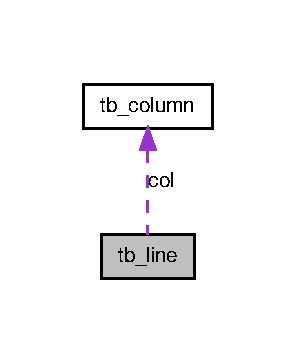
\includegraphics[width=142pt]{structtb__line__coll__graph}
\end{center}
\end{figure}
\subsection*{Public Attributes}
\begin{DoxyCompactItemize}
\item 
\hyperlink{structtb__column}{tb\_\-column} $\ast$ \hyperlink{structtb__line_a696513af3da4418db8d49ee318a0055b}{col}
\item 
int \hyperlink{structtb__line_adc05d4116a10f0cd23f22f9be0f7495e}{n\_\-col}
\end{DoxyCompactItemize}


\subsection{Detailed Description}


Definition at line 9 of file dissect.h.



\subsection{Member Data Documentation}
\hypertarget{structtb__line_a696513af3da4418db8d49ee318a0055b}{
\index{tb\_\-line@{tb\_\-line}!col@{col}}
\index{col@{col}!tb_line@{tb\_\-line}}
\subsubsection[{col}]{\setlength{\rightskip}{0pt plus 5cm}{\bf tb\_\-column} $\ast$ {\bf tb\_\-line::col}}}
\label{structtb__line_a696513af3da4418db8d49ee318a0055b}


Definition at line 10 of file dissect.h.

\hypertarget{structtb__line_adc05d4116a10f0cd23f22f9be0f7495e}{
\index{tb\_\-line@{tb\_\-line}!n\_\-col@{n\_\-col}}
\index{n\_\-col@{n\_\-col}!tb_line@{tb\_\-line}}
\subsubsection[{n\_\-col}]{\setlength{\rightskip}{0pt plus 5cm}int {\bf tb\_\-line::n\_\-col}}}
\label{structtb__line_adc05d4116a10f0cd23f22f9be0f7495e}


Definition at line 11 of file dissect.h.



The documentation for this struct was generated from the following files:\begin{DoxyCompactItemize}
\item 
src/libmalelf/include/malelf/\hyperlink{dissect_8h}{dissect.h}\item 
src/libmalelf/include/malelf/\hyperlink{print__table_8h}{print\_\-table.h}\end{DoxyCompactItemize}

\chapter{File Documentation}
\hypertarget{copy_8c}{
\section{src/libmalelf/copy.c File Reference}
\label{copy_8c}\index{src/libmalelf/copy.c@{src/libmalelf/copy.c}}
}

\hypertarget{disas_8c}{
\section{src/libmalelf/disas.c File Reference}
\label{disas_8c}\index{src/libmalelf/disas.c@{src/libmalelf/disas.c}}
}
{\ttfamily \#include $<$errno.h$>$}\par
{\ttfamily \#include $<$fcntl.h$>$}\par
{\ttfamily \#include $<$stdlib.h$>$}\par
{\ttfamily \#include $<$string.h$>$}\par
{\ttfamily \#include $<$stdio.h$>$}\par
{\ttfamily \#include $<$sys/mman.h$>$}\par
{\ttfamily \#include $<$sys/stat.h$>$}\par
{\ttfamily \#include $<$sys/types.h$>$}\par
{\ttfamily \#include $<$unistd.h$>$}\par
{\ttfamily \#include $<$inttypes.h$>$}\par
{\ttfamily \#include $<$beaengine/BeaEngine.h$>$}\par
{\ttfamily \#include $<$malelf/defines.h$>$}\par
{\ttfamily \#include $<$malelf/error.h$>$}\par
{\ttfamily \#include $<$malelf/disas.h$>$}\par
{\ttfamily \#include $<$malelf/util.h$>$}\par
{\ttfamily \#include $<$malelf/object.h$>$}\par
Include dependency graph for disas.c:\nopagebreak
\begin{figure}[H]
\begin{center}
\leavevmode
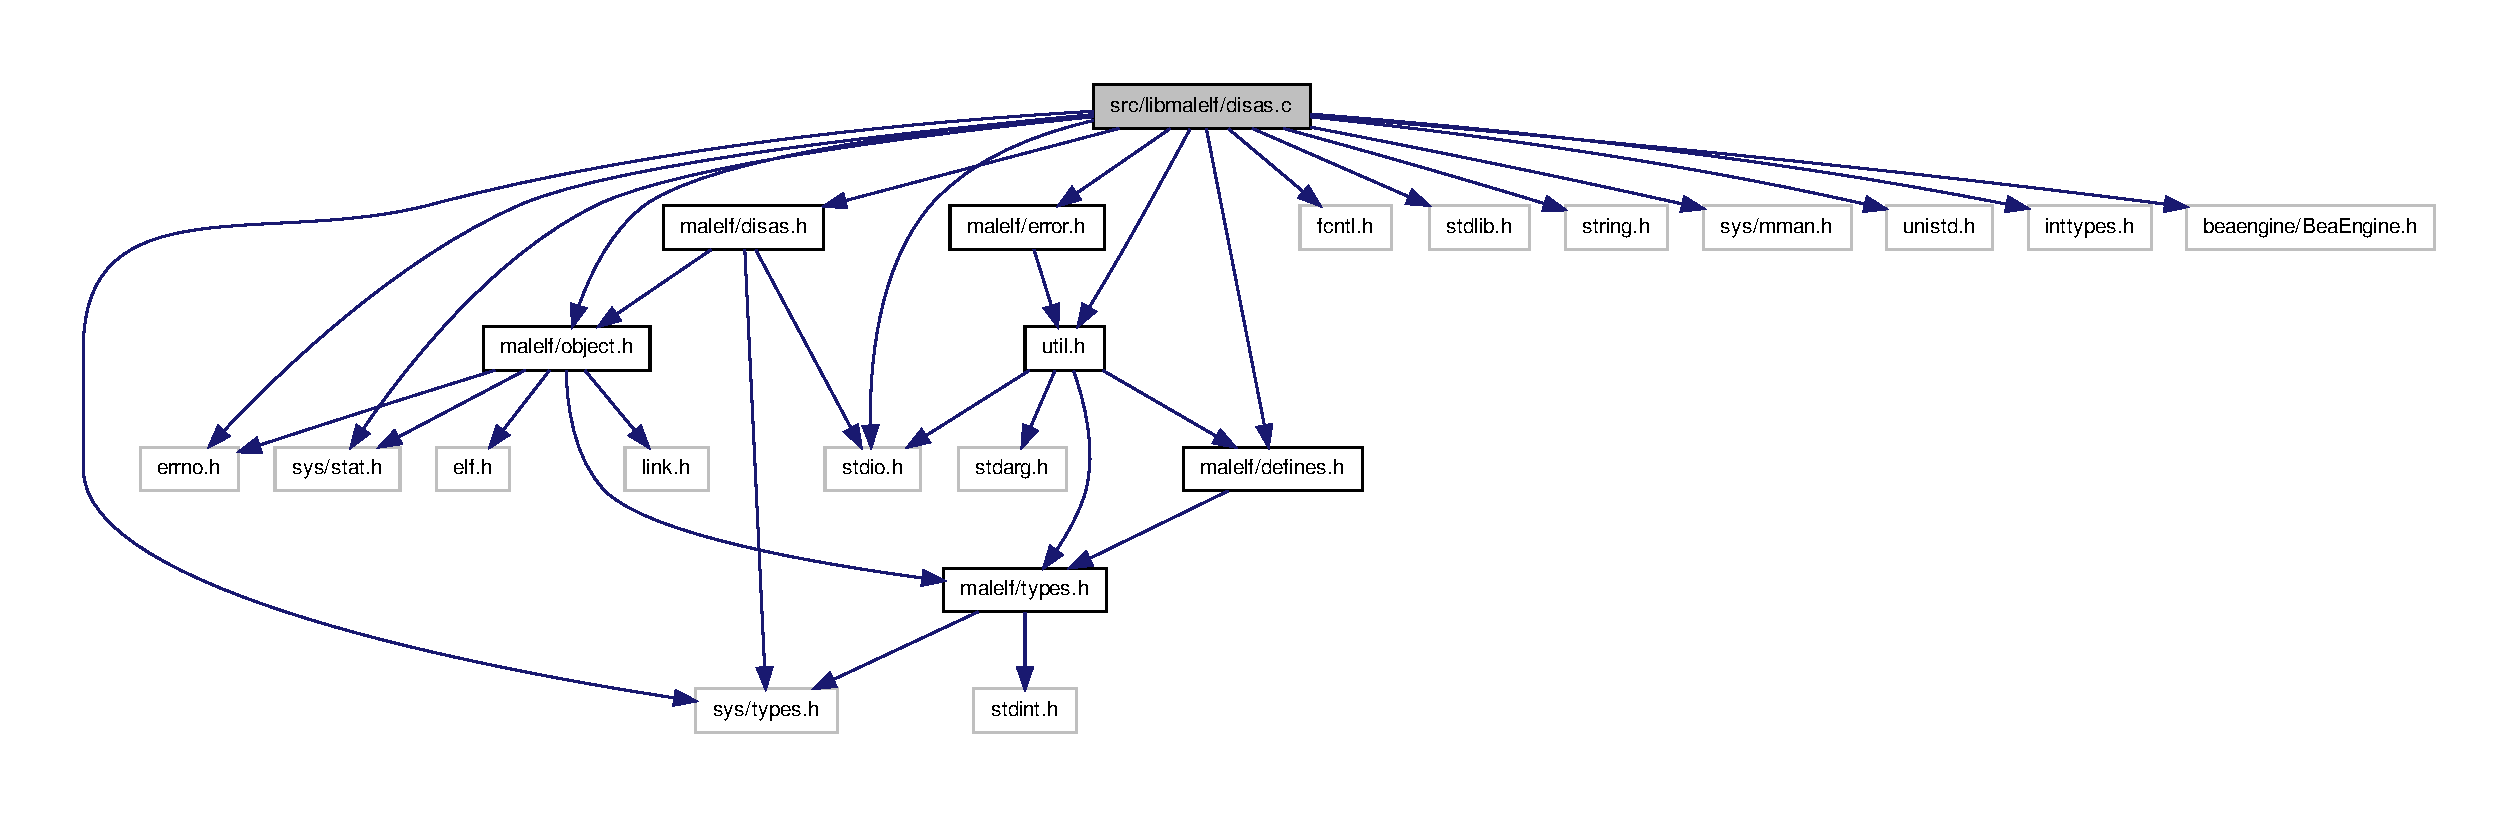
\includegraphics[width=400pt]{disas_8c__incl}
\end{center}
\end{figure}
\subsection*{Defines}
\begin{DoxyCompactItemize}
\item 
\#define \hyperlink{disas_8c_a1bf6c868670adced4756500721b9d6ae}{\_\-P}~malelf\_\-print
\item 
\#define \hyperlink{disas_8c_afb517d6fab1f8049d683a0953ddd27e8}{\_\-PDIRECTIVE}~\_\-P
\item 
\#define \hyperlink{disas_8c_a3257f30baf0314af3f830124b55ee8d6}{\_\-PISN}~malelf\_\-print\_\-isn
\item 
\#define \hyperlink{disas_8c_ad6b0103f7c81805f5e803bbd348510b0}{\_\-PLABEL}~\_\-P
\end{DoxyCompactItemize}
\subsection*{Functions}
\begin{DoxyCompactItemize}
\item 
int \hyperlink{disas_8c_a914cd9d658cbf28142de1bc2239d5c90}{malelf\_\-print\_\-isn} (FILE $\ast$fd, const char $\ast$format,...)
\item 
\hyperlink{types_8h_aacb1ea6e27efde1c708a8bc4b56ee1a2}{\_\-i32} \hyperlink{disas_8c_a038ee7ce644f9c84afa9eda088a88a19}{malelf\_\-disas\_\-ehdr} (ElfW(Ehdr)$\ast$ehdr, FILE $\ast$fd)
\item 
\hyperlink{types_8h_aacb1ea6e27efde1c708a8bc4b56ee1a2}{\_\-i32} \hyperlink{disas_8c_a443fe5760c50193cf071c934c092e298}{malelf\_\-disas\_\-phdr} (\hyperlink{structmalelf__elf__t}{malelf\_\-elf\_\-t} $\ast$elf, FILE $\ast$fd)
\item 
\hyperlink{types_8h_aacb1ea6e27efde1c708a8bc4b56ee1a2}{\_\-i32} \hyperlink{disas_8c_aaf83c95eafd6ebf3615de15015928785}{malelf\_\-disas\_\-sht} (\hyperlink{structmalelf__object}{malelf\_\-object} $\ast$obj, FILE $\ast$fd)
\item 
\hyperlink{types_8h_aacb1ea6e27efde1c708a8bc4b56ee1a2}{\_\-i32} \hyperlink{disas_8c_a0b48f10e02dc75265d8dcfac19320e20}{malelf\_\-disas\_\-program} (\hyperlink{structmalelf__object}{malelf\_\-object} $\ast$obj, FILE $\ast$fd)
\item 
\hyperlink{types_8h_aacb1ea6e27efde1c708a8bc4b56ee1a2}{\_\-i32} \hyperlink{disas_8c_af9ff556491cf0633735f10e5c4994f21}{malelf\_\-disas\_\-flat} (\hyperlink{structmalelf__object}{malelf\_\-object} $\ast$obj, FILE $\ast$fd)
\item 
\hyperlink{types_8h_aacb1ea6e27efde1c708a8bc4b56ee1a2}{\_\-i32} \hyperlink{disas_8c_ab01161abb4cd223636c52bac74fc16eb}{malelf\_\-disas\_\-section} (\hyperlink{structmalelf__object}{malelf\_\-object} $\ast$obj, char $\ast$section, FILE $\ast$fd)
\item 
\hyperlink{types_8h_aacb1ea6e27efde1c708a8bc4b56ee1a2}{\_\-i32} \hyperlink{disas_8c_a6e603fc09032b4fad1dd486b3381ee50}{malelf\_\-disas} (\hyperlink{structmalelf__object}{malelf\_\-object} $\ast$input, FILE $\ast$outfd)
\end{DoxyCompactItemize}
\subsection*{Variables}
\begin{DoxyCompactItemize}
\item 
\hyperlink{types_8h_af2b0f13cffd24f6dddf794ae0c7472b4}{\_\-u8} \hyperlink{disas_8c_a9832bf9a14bd3b9656e7be172ac16c9b}{malelf\_\-quiet\_\-mode}
\begin{DoxyCompactList}\small\item\em Quiet mode. \end{DoxyCompactList}\end{DoxyCompactItemize}


\subsection{Define Documentation}
\hypertarget{disas_8c_a1bf6c868670adced4756500721b9d6ae}{
\index{disas.c@{disas.c}!\_\-P@{\_\-P}}
\index{\_\-P@{\_\-P}!disas.c@{disas.c}}
\subsubsection[{\_\-P}]{\setlength{\rightskip}{0pt plus 5cm}\#define \_\-P~malelf\_\-print}}
\label{disas_8c_a1bf6c868670adced4756500721b9d6ae}


Definition at line 22 of file disas.c.

\hypertarget{disas_8c_afb517d6fab1f8049d683a0953ddd27e8}{
\index{disas.c@{disas.c}!\_\-PDIRECTIVE@{\_\-PDIRECTIVE}}
\index{\_\-PDIRECTIVE@{\_\-PDIRECTIVE}!disas.c@{disas.c}}
\subsubsection[{\_\-PDIRECTIVE}]{\setlength{\rightskip}{0pt plus 5cm}\#define \_\-PDIRECTIVE~\_\-P}}
\label{disas_8c_afb517d6fab1f8049d683a0953ddd27e8}


Definition at line 23 of file disas.c.

\hypertarget{disas_8c_a3257f30baf0314af3f830124b55ee8d6}{
\index{disas.c@{disas.c}!\_\-PISN@{\_\-PISN}}
\index{\_\-PISN@{\_\-PISN}!disas.c@{disas.c}}
\subsubsection[{\_\-PISN}]{\setlength{\rightskip}{0pt plus 5cm}\#define \_\-PISN~malelf\_\-print\_\-isn}}
\label{disas_8c_a3257f30baf0314af3f830124b55ee8d6}


Definition at line 24 of file disas.c.

\hypertarget{disas_8c_ad6b0103f7c81805f5e803bbd348510b0}{
\index{disas.c@{disas.c}!\_\-PLABEL@{\_\-PLABEL}}
\index{\_\-PLABEL@{\_\-PLABEL}!disas.c@{disas.c}}
\subsubsection[{\_\-PLABEL}]{\setlength{\rightskip}{0pt plus 5cm}\#define \_\-PLABEL~\_\-P}}
\label{disas_8c_ad6b0103f7c81805f5e803bbd348510b0}


Definition at line 25 of file disas.c.



\subsection{Function Documentation}
\hypertarget{disas_8c_a6e603fc09032b4fad1dd486b3381ee50}{
\index{disas.c@{disas.c}!malelf\_\-disas@{malelf\_\-disas}}
\index{malelf\_\-disas@{malelf\_\-disas}!disas.c@{disas.c}}
\subsubsection[{malelf\_\-disas}]{\setlength{\rightskip}{0pt plus 5cm}{\bf \_\-i32} malelf\_\-disas (
\begin{DoxyParamCaption}
\item[{{\bf malelf\_\-object} $\ast$}]{input, }
\item[{FILE $\ast$}]{outfd}
\end{DoxyParamCaption}
)}}
\label{disas_8c_a6e603fc09032b4fad1dd486b3381ee50}


Definition at line 288 of file disas.c.

\hypertarget{disas_8c_a038ee7ce644f9c84afa9eda088a88a19}{
\index{disas.c@{disas.c}!malelf\_\-disas\_\-ehdr@{malelf\_\-disas\_\-ehdr}}
\index{malelf\_\-disas\_\-ehdr@{malelf\_\-disas\_\-ehdr}!disas.c@{disas.c}}
\subsubsection[{malelf\_\-disas\_\-ehdr}]{\setlength{\rightskip}{0pt plus 5cm}{\bf \_\-i32} malelf\_\-disas\_\-ehdr (
\begin{DoxyParamCaption}
\item[{ElfW(Ehdr)$\ast$}]{ehdr, }
\item[{FILE $\ast$}]{fd}
\end{DoxyParamCaption}
)}}
\label{disas_8c_a038ee7ce644f9c84afa9eda088a88a19}


Definition at line 33 of file disas.c.

\hypertarget{disas_8c_af9ff556491cf0633735f10e5c4994f21}{
\index{disas.c@{disas.c}!malelf\_\-disas\_\-flat@{malelf\_\-disas\_\-flat}}
\index{malelf\_\-disas\_\-flat@{malelf\_\-disas\_\-flat}!disas.c@{disas.c}}
\subsubsection[{malelf\_\-disas\_\-flat}]{\setlength{\rightskip}{0pt plus 5cm}{\bf \_\-i32} malelf\_\-disas\_\-flat (
\begin{DoxyParamCaption}
\item[{{\bf malelf\_\-object} $\ast$}]{obj, }
\item[{FILE $\ast$}]{fd}
\end{DoxyParamCaption}
)}}
\label{disas_8c_af9ff556491cf0633735f10e5c4994f21}


Definition at line 190 of file disas.c.

\hypertarget{disas_8c_a443fe5760c50193cf071c934c092e298}{
\index{disas.c@{disas.c}!malelf\_\-disas\_\-phdr@{malelf\_\-disas\_\-phdr}}
\index{malelf\_\-disas\_\-phdr@{malelf\_\-disas\_\-phdr}!disas.c@{disas.c}}
\subsubsection[{malelf\_\-disas\_\-phdr}]{\setlength{\rightskip}{0pt plus 5cm}{\bf \_\-i32} malelf\_\-disas\_\-phdr (
\begin{DoxyParamCaption}
\item[{{\bf malelf\_\-elf\_\-t} $\ast$}]{elf, }
\item[{FILE $\ast$}]{fd}
\end{DoxyParamCaption}
)}}
\label{disas_8c_a443fe5760c50193cf071c934c092e298}


Definition at line 76 of file disas.c.

\hypertarget{disas_8c_a0b48f10e02dc75265d8dcfac19320e20}{
\index{disas.c@{disas.c}!malelf\_\-disas\_\-program@{malelf\_\-disas\_\-program}}
\index{malelf\_\-disas\_\-program@{malelf\_\-disas\_\-program}!disas.c@{disas.c}}
\subsubsection[{malelf\_\-disas\_\-program}]{\setlength{\rightskip}{0pt plus 5cm}{\bf \_\-i32} malelf\_\-disas\_\-program (
\begin{DoxyParamCaption}
\item[{{\bf malelf\_\-object} $\ast$}]{obj, }
\item[{FILE $\ast$}]{fd}
\end{DoxyParamCaption}
)}}
\label{disas_8c_a0b48f10e02dc75265d8dcfac19320e20}


Definition at line 128 of file disas.c.

\hypertarget{disas_8c_ab01161abb4cd223636c52bac74fc16eb}{
\index{disas.c@{disas.c}!malelf\_\-disas\_\-section@{malelf\_\-disas\_\-section}}
\index{malelf\_\-disas\_\-section@{malelf\_\-disas\_\-section}!disas.c@{disas.c}}
\subsubsection[{malelf\_\-disas\_\-section}]{\setlength{\rightskip}{0pt plus 5cm}{\bf \_\-i32} malelf\_\-disas\_\-section (
\begin{DoxyParamCaption}
\item[{{\bf malelf\_\-object} $\ast$}]{obj, }
\item[{char $\ast$}]{section, }
\item[{FILE $\ast$}]{fd}
\end{DoxyParamCaption}
)}}
\label{disas_8c_ab01161abb4cd223636c52bac74fc16eb}


Definition at line 226 of file disas.c.

\hypertarget{disas_8c_aaf83c95eafd6ebf3615de15015928785}{
\index{disas.c@{disas.c}!malelf\_\-disas\_\-sht@{malelf\_\-disas\_\-sht}}
\index{malelf\_\-disas\_\-sht@{malelf\_\-disas\_\-sht}!disas.c@{disas.c}}
\subsubsection[{malelf\_\-disas\_\-sht}]{\setlength{\rightskip}{0pt plus 5cm}{\bf \_\-i32} malelf\_\-disas\_\-sht (
\begin{DoxyParamCaption}
\item[{{\bf malelf\_\-object} $\ast$}]{obj, }
\item[{FILE $\ast$}]{fd}
\end{DoxyParamCaption}
)}}
\label{disas_8c_aaf83c95eafd6ebf3615de15015928785}


Definition at line 100 of file disas.c.

\hypertarget{disas_8c_a914cd9d658cbf28142de1bc2239d5c90}{
\index{disas.c@{disas.c}!malelf\_\-print\_\-isn@{malelf\_\-print\_\-isn}}
\index{malelf\_\-print\_\-isn@{malelf\_\-print\_\-isn}!disas.c@{disas.c}}
\subsubsection[{malelf\_\-print\_\-isn}]{\setlength{\rightskip}{0pt plus 5cm}int malelf\_\-print\_\-isn (
\begin{DoxyParamCaption}
\item[{FILE $\ast$}]{fd, }
\item[{const char $\ast$}]{format, }
\item[{}]{...}
\end{DoxyParamCaption}
)}}
\label{disas_8c_a914cd9d658cbf28142de1bc2239d5c90}


Definition at line 27 of file disas.c.



\subsection{Variable Documentation}
\hypertarget{disas_8c_a9832bf9a14bd3b9656e7be172ac16c9b}{
\index{disas.c@{disas.c}!malelf\_\-quiet\_\-mode@{malelf\_\-quiet\_\-mode}}
\index{malelf\_\-quiet\_\-mode@{malelf\_\-quiet\_\-mode}!disas.c@{disas.c}}
\subsubsection[{malelf\_\-quiet\_\-mode}]{\setlength{\rightskip}{0pt plus 5cm}{\bf \_\-u8} {\bf malelf\_\-quiet\_\-mode}}}
\label{disas_8c_a9832bf9a14bd3b9656e7be172ac16c9b}


Quiet mode. 

Enable quiet mode 

Definition at line 54 of file object.c.


\hypertarget{dissect_8c}{
\section{src/libmalelf/dissect.c File Reference}
\label{dissect_8c}\index{src/libmalelf/dissect.c@{src/libmalelf/dissect.c}}
}
{\ttfamily \#include $<$stdio.h$>$}\par
{\ttfamily \#include $<$stdlib.h$>$}\par
{\ttfamily \#include $<$string.h$>$}\par
{\ttfamily \#include $<$assert.h$>$}\par
{\ttfamily \#include $<$link.h$>$}\par
{\ttfamily \#include $<$malelf/defines.h$>$}\par
{\ttfamily \#include $<$malelf/object.h$>$}\par
{\ttfamily \#include $<$malelf/error.h$>$}\par
{\ttfamily \#include $<$malelf/util.h$>$}\par
{\ttfamily \#include $<$malelf/dissect.h$>$}\par
{\ttfamily \#include $<$malelf/print\_\-table.h$>$}\par
Include dependency graph for dissect.c:\nopagebreak
\begin{figure}[H]
\begin{center}
\leavevmode
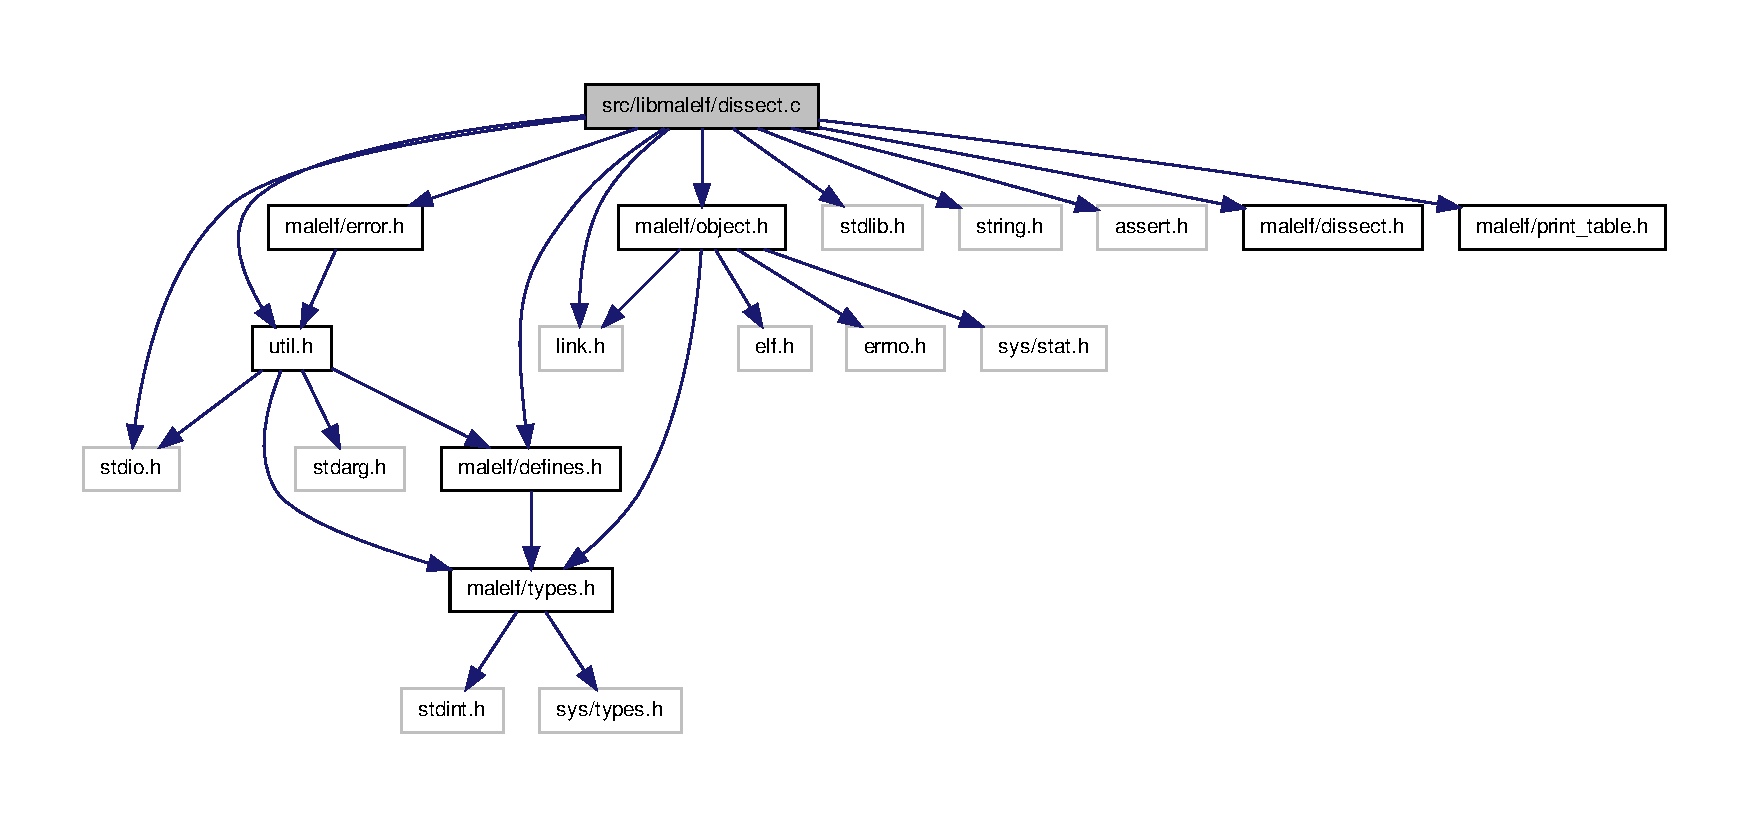
\includegraphics[width=400pt]{dissect_8c__incl}
\end{center}
\end{figure}
\subsection*{Functions}
\begin{DoxyCompactItemize}
\item 
\hyperlink{types_8h_aacb1ea6e27efde1c708a8bc4b56ee1a2}{\_\-i32} \hyperlink{dissect_8c_a6fad0db775504c32cd2bbdbb984902ce}{malelf\_\-sections\_\-exec} (\hyperlink{structmalelf__object}{malelf\_\-object} $\ast$elf\_\-obj, \hyperlink{types_8h_aacb1ea6e27efde1c708a8bc4b56ee1a2}{\_\-i32}($\ast$callback)(char $\ast$sect\_\-n, char $\ast$sect\_\-t, void $\ast$arg), void $\ast$arg)
\item 
void \hyperlink{dissect_8c_a2f7affe0bdf4f8c32b8b05c344131567}{pretty\_\-print\_\-elf\_\-header} (ElfW(Ehdr)$\ast$header)
\item 
void \hyperlink{dissect_8c_a572189fd54f1c3e152f237a63d863823}{pretty\_\-print\_\-pht} (ElfW(Ehdr)$\ast$header, ElfW(Phdr)$\ast$pheaders)
\item 
void \hyperlink{dissect_8c_a9650c93bd5c6d16d810825a8206b70fd}{pretty\_\-print\_\-sht} (\hyperlink{structmalelf__object}{malelf\_\-object} $\ast$elf, ElfW(Ehdr)$\ast$header, ElfW(Shdr)$\ast$sections)
\item 
void \hyperlink{dissect_8c_aed66520a6daf153a1259eebb41348027}{pretty\_\-print\_\-strtab} (\hyperlink{structmalelf__object}{malelf\_\-object} $\ast$elf, ElfW(Ehdr)$\ast$header, ElfW(Shdr)$\ast$sections)
\end{DoxyCompactItemize}


\subsection{Function Documentation}
\hypertarget{dissect_8c_a6fad0db775504c32cd2bbdbb984902ce}{
\index{dissect.c@{dissect.c}!malelf\_\-sections\_\-exec@{malelf\_\-sections\_\-exec}}
\index{malelf\_\-sections\_\-exec@{malelf\_\-sections\_\-exec}!dissect.c@{dissect.c}}
\subsubsection[{malelf\_\-sections\_\-exec}]{\setlength{\rightskip}{0pt plus 5cm}{\bf \_\-i32} malelf\_\-sections\_\-exec (
\begin{DoxyParamCaption}
\item[{{\bf malelf\_\-object} $\ast$}]{elf\_\-obj, }
\item[{{\bf \_\-i32}($\ast$)(char $\ast$sect\_\-n, char $\ast$sect\_\-t, void $\ast$arg)}]{callback, }
\item[{void $\ast$}]{arg}
\end{DoxyParamCaption}
)}}
\label{dissect_8c_a6fad0db775504c32cd2bbdbb984902ce}


Definition at line 14 of file dissect.c.

\hypertarget{dissect_8c_a2f7affe0bdf4f8c32b8b05c344131567}{
\index{dissect.c@{dissect.c}!pretty\_\-print\_\-elf\_\-header@{pretty\_\-print\_\-elf\_\-header}}
\index{pretty\_\-print\_\-elf\_\-header@{pretty\_\-print\_\-elf\_\-header}!dissect.c@{dissect.c}}
\subsubsection[{pretty\_\-print\_\-elf\_\-header}]{\setlength{\rightskip}{0pt plus 5cm}void pretty\_\-print\_\-elf\_\-header (
\begin{DoxyParamCaption}
\item[{ElfW(Ehdr)$\ast$}]{header}
\end{DoxyParamCaption}
)}}
\label{dissect_8c_a2f7affe0bdf4f8c32b8b05c344131567}


Definition at line 63 of file dissect.c.

\hypertarget{dissect_8c_a572189fd54f1c3e152f237a63d863823}{
\index{dissect.c@{dissect.c}!pretty\_\-print\_\-pht@{pretty\_\-print\_\-pht}}
\index{pretty\_\-print\_\-pht@{pretty\_\-print\_\-pht}!dissect.c@{dissect.c}}
\subsubsection[{pretty\_\-print\_\-pht}]{\setlength{\rightskip}{0pt plus 5cm}void pretty\_\-print\_\-pht (
\begin{DoxyParamCaption}
\item[{ElfW(Ehdr)$\ast$}]{header, }
\item[{ElfW(Phdr)$\ast$}]{pheaders}
\end{DoxyParamCaption}
)}}
\label{dissect_8c_a572189fd54f1c3e152f237a63d863823}


Definition at line 157 of file dissect.c.

\hypertarget{dissect_8c_a9650c93bd5c6d16d810825a8206b70fd}{
\index{dissect.c@{dissect.c}!pretty\_\-print\_\-sht@{pretty\_\-print\_\-sht}}
\index{pretty\_\-print\_\-sht@{pretty\_\-print\_\-sht}!dissect.c@{dissect.c}}
\subsubsection[{pretty\_\-print\_\-sht}]{\setlength{\rightskip}{0pt plus 5cm}void pretty\_\-print\_\-sht (
\begin{DoxyParamCaption}
\item[{{\bf malelf\_\-object} $\ast$}]{elf, }
\item[{ElfW(Ehdr)$\ast$}]{header, }
\item[{ElfW(Shdr)$\ast$}]{sections}
\end{DoxyParamCaption}
)}}
\label{dissect_8c_a9650c93bd5c6d16d810825a8206b70fd}


Definition at line 196 of file dissect.c.

\hypertarget{dissect_8c_aed66520a6daf153a1259eebb41348027}{
\index{dissect.c@{dissect.c}!pretty\_\-print\_\-strtab@{pretty\_\-print\_\-strtab}}
\index{pretty\_\-print\_\-strtab@{pretty\_\-print\_\-strtab}!dissect.c@{dissect.c}}
\subsubsection[{pretty\_\-print\_\-strtab}]{\setlength{\rightskip}{0pt plus 5cm}void pretty\_\-print\_\-strtab (
\begin{DoxyParamCaption}
\item[{{\bf malelf\_\-object} $\ast$}]{elf, }
\item[{ElfW(Ehdr)$\ast$}]{header, }
\item[{ElfW(Shdr)$\ast$}]{sections}
\end{DoxyParamCaption}
)}}
\label{dissect_8c_aed66520a6daf153a1259eebb41348027}
Algorithm based on Elfrw function elfr\_\-symtable\_\-dump at (\href{https://github.com/felipensp/ELFrw}{\tt https://github.com/felipensp/ELFrw})

TODO: $\ast$rewrite this$\ast$ 

Definition at line 257 of file dissect.c.


\hypertarget{error_8c}{
\section{src/libmalelf/error.c File Reference}
\label{error_8c}\index{src/libmalelf/error.c@{src/libmalelf/error.c}}
}
{\ttfamily \#include $<$stdio.h$>$}\par
{\ttfamily \#include $<$stdlib.h$>$}\par
{\ttfamily \#include $<$string.h$>$}\par
{\ttfamily \#include \char`\"{}malelf/error.h\char`\"{}}\par
Include dependency graph for error.c:\nopagebreak
\begin{figure}[H]
\begin{center}
\leavevmode
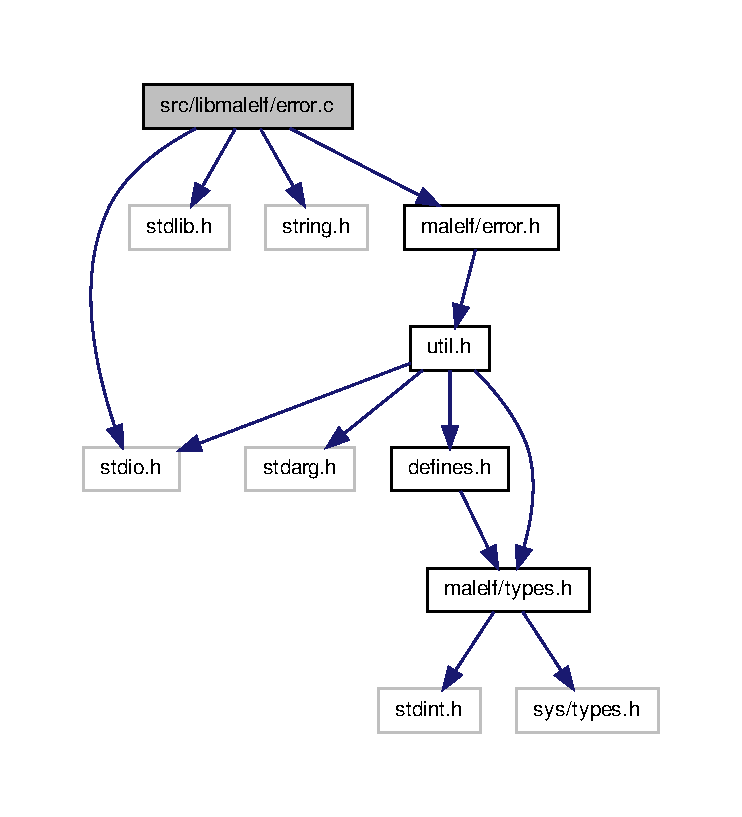
\includegraphics[width=356pt]{error_8c__incl}
\end{center}
\end{figure}
\subsection*{Functions}
\begin{DoxyCompactItemize}
\item 
const char $\ast$ \hyperlink{error_8c_af225ce01f3f2709e264c7036e813c3b1}{malelf\_\-strerror} (int code)
\item 
void \hyperlink{error_8c_ad60f880160e465f8f99c9d4ad8c95d21}{\_\-malelf\_\-perror} (int code, const char $\ast$func, const char $\ast$file, int line)
\end{DoxyCompactItemize}
\subsection*{Variables}
\begin{DoxyCompactItemize}
\item 
const char $\ast$ \hyperlink{error_8c_a93e57a1f4365443157657d4050705a42}{malelf\_\-strerr} \mbox{[}$\,$\mbox{]}
\end{DoxyCompactItemize}


\subsection{Function Documentation}
\hypertarget{error_8c_ad60f880160e465f8f99c9d4ad8c95d21}{
\index{error.c@{error.c}!\_\-malelf\_\-perror@{\_\-malelf\_\-perror}}
\index{\_\-malelf\_\-perror@{\_\-malelf\_\-perror}!error.c@{error.c}}
\subsubsection[{\_\-malelf\_\-perror}]{\setlength{\rightskip}{0pt plus 5cm}void \_\-malelf\_\-perror (
\begin{DoxyParamCaption}
\item[{int}]{code, }
\item[{const char $\ast$}]{func, }
\item[{const char $\ast$}]{file, }
\item[{int}]{line}
\end{DoxyParamCaption}
)}}
\label{error_8c_ad60f880160e465f8f99c9d4ad8c95d21}


Definition at line 24 of file error.c.

\hypertarget{error_8c_af225ce01f3f2709e264c7036e813c3b1}{
\index{error.c@{error.c}!malelf\_\-strerror@{malelf\_\-strerror}}
\index{malelf\_\-strerror@{malelf\_\-strerror}!error.c@{error.c}}
\subsubsection[{malelf\_\-strerror}]{\setlength{\rightskip}{0pt plus 5cm}const char$\ast$ malelf\_\-strerror (
\begin{DoxyParamCaption}
\item[{int}]{code}
\end{DoxyParamCaption}
)}}
\label{error_8c_af225ce01f3f2709e264c7036e813c3b1}


Definition at line 20 of file error.c.



\subsection{Variable Documentation}
\hypertarget{error_8c_a93e57a1f4365443157657d4050705a42}{
\index{error.c@{error.c}!malelf\_\-strerr@{malelf\_\-strerr}}
\index{malelf\_\-strerr@{malelf\_\-strerr}!error.c@{error.c}}
\subsubsection[{malelf\_\-strerr}]{\setlength{\rightskip}{0pt plus 5cm}const char$\ast$ {\bf malelf\_\-strerr}\mbox{[}$\,$\mbox{]}}}
\label{error_8c_a93e57a1f4365443157657d4050705a42}
{\bfseries Initial value:}
\begin{DoxyCode}
 {
    "Unknow error", 
    "File already closed",
    "Error allocating memory",
    "Binary is NOT ELF",
    "Binary is corrupted",
    "Binary has suspect section names",
    "Missing magic bytes in malware",
    "Invalid offset for returned entry point in malware",
    "Disassembly error."
    
}
\end{DoxyCode}


Definition at line 7 of file error.c.


\hypertarget{header__types_8inc}{
\section{src/libmalelf/header\_\-types.inc File Reference}
\label{header__types_8inc}\index{src/libmalelf/header\_\-types.inc@{src/libmalelf/header\_\-types.inc}}
}
This graph shows which files directly or indirectly include this file:\nopagebreak
\begin{figure}[H]
\begin{center}
\leavevmode
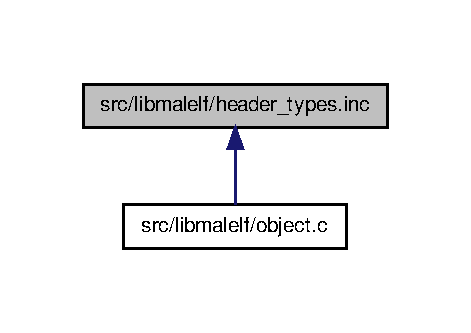
\includegraphics[width=226pt]{header__types_8inc__dep__incl}
\end{center}
\end{figure}

\hypertarget{defines_8h}{
\section{src/libmalelf/include/malelf/defines.h File Reference}
\label{defines_8h}\index{src/libmalelf/include/malelf/defines.h@{src/libmalelf/include/malelf/defines.h}}
}
{\ttfamily \#include $<$malelf/types.h$>$}\par
Include dependency graph for defines.h:\nopagebreak
\begin{figure}[H]
\begin{center}
\leavevmode
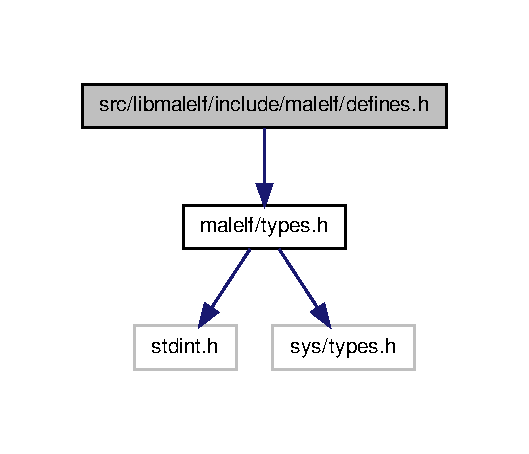
\includegraphics[width=254pt]{defines_8h__incl}
\end{center}
\end{figure}
This graph shows which files directly or indirectly include this file:\nopagebreak
\begin{figure}[H]
\begin{center}
\leavevmode
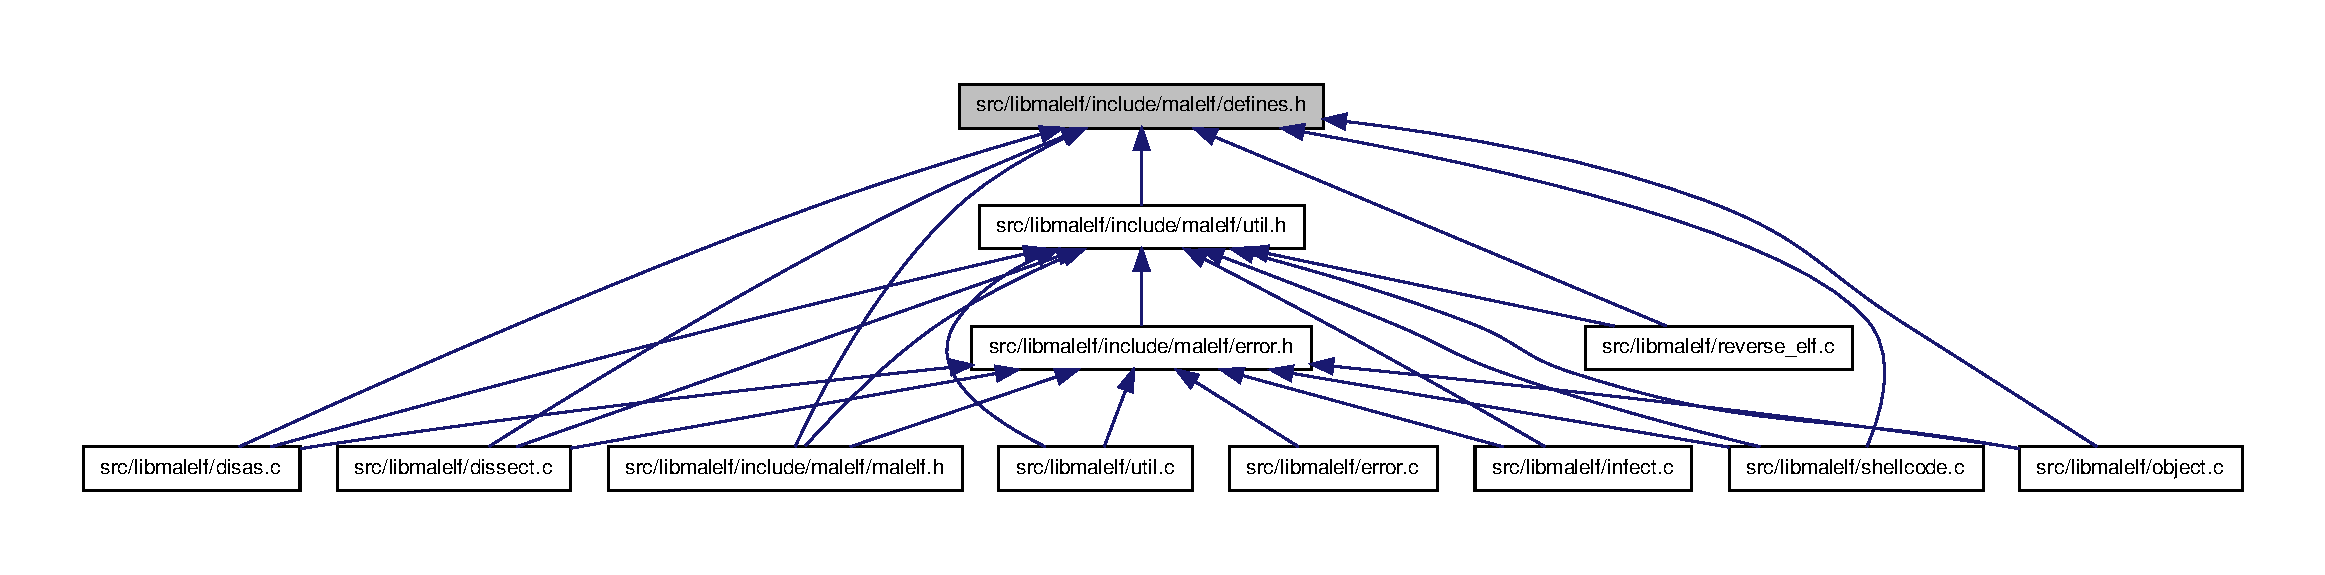
\includegraphics[width=400pt]{defines_8h__dep__incl}
\end{center}
\end{figure}
\subsection*{Defines}
\begin{DoxyCompactItemize}
\item 
\#define \hyperlink{defines_8h_ac361f570cbcab8a48af802a7ef1f6370}{MALELF\_\-READWRITE}~0
\item 
\#define \hyperlink{defines_8h_a58ae9da477121fa6dcc7f66dbfd1eb08}{MALELF\_\-READONLY}~1
\end{DoxyCompactItemize}
\subsection*{Variables}
\begin{DoxyCompactItemize}
\item 
\hyperlink{types_8h_af2b0f13cffd24f6dddf794ae0c7472b4}{\_\-u8} \hyperlink{defines_8h_a9832bf9a14bd3b9656e7be172ac16c9b}{malelf\_\-quiet\_\-mode}
\begin{DoxyCompactList}\small\item\em Quiet mode. \end{DoxyCompactList}\item 
\hyperlink{types_8h_af2b0f13cffd24f6dddf794ae0c7472b4}{\_\-u8} \hyperlink{defines_8h_acd6ab4d02330caecbb7e6e11930b31b3}{malelf\_\-verbose\_\-mode}
\end{DoxyCompactItemize}


\subsection{Define Documentation}
\hypertarget{defines_8h_a58ae9da477121fa6dcc7f66dbfd1eb08}{
\index{defines.h@{defines.h}!MALELF\_\-READONLY@{MALELF\_\-READONLY}}
\index{MALELF\_\-READONLY@{MALELF\_\-READONLY}!defines.h@{defines.h}}
\subsubsection[{MALELF\_\-READONLY}]{\setlength{\rightskip}{0pt plus 5cm}\#define MALELF\_\-READONLY~1}}
\label{defines_8h_a58ae9da477121fa6dcc7f66dbfd1eb08}


Definition at line 5 of file defines.h.

\hypertarget{defines_8h_ac361f570cbcab8a48af802a7ef1f6370}{
\index{defines.h@{defines.h}!MALELF\_\-READWRITE@{MALELF\_\-READWRITE}}
\index{MALELF\_\-READWRITE@{MALELF\_\-READWRITE}!defines.h@{defines.h}}
\subsubsection[{MALELF\_\-READWRITE}]{\setlength{\rightskip}{0pt plus 5cm}\#define MALELF\_\-READWRITE~0}}
\label{defines_8h_ac361f570cbcab8a48af802a7ef1f6370}


Definition at line 4 of file defines.h.



\subsection{Variable Documentation}
\hypertarget{defines_8h_a9832bf9a14bd3b9656e7be172ac16c9b}{
\index{defines.h@{defines.h}!malelf\_\-quiet\_\-mode@{malelf\_\-quiet\_\-mode}}
\index{malelf\_\-quiet\_\-mode@{malelf\_\-quiet\_\-mode}!defines.h@{defines.h}}
\subsubsection[{malelf\_\-quiet\_\-mode}]{\setlength{\rightskip}{0pt plus 5cm}{\bf \_\-u8} {\bf malelf\_\-quiet\_\-mode}}}
\label{defines_8h_a9832bf9a14bd3b9656e7be172ac16c9b}


Quiet mode. 

Enable quiet mode 

Definition at line 54 of file object.c.

\hypertarget{defines_8h_acd6ab4d02330caecbb7e6e11930b31b3}{
\index{defines.h@{defines.h}!malelf\_\-verbose\_\-mode@{malelf\_\-verbose\_\-mode}}
\index{malelf\_\-verbose\_\-mode@{malelf\_\-verbose\_\-mode}!defines.h@{defines.h}}
\subsubsection[{malelf\_\-verbose\_\-mode}]{\setlength{\rightskip}{0pt plus 5cm}{\bf \_\-u8} {\bf malelf\_\-verbose\_\-mode}}}
\label{defines_8h_acd6ab4d02330caecbb7e6e11930b31b3}

\hypertarget{disas_8h}{
\section{src/libmalelf/include/malelf/disas.h File Reference}
\label{disas_8h}\index{src/libmalelf/include/malelf/disas.h@{src/libmalelf/include/malelf/disas.h}}
}
{\ttfamily \#include $<$stdio.h$>$}\par
{\ttfamily \#include $<$sys/types.h$>$}\par
{\ttfamily \#include \char`\"{}malelf/object.h\char`\"{}}\par
Include dependency graph for disas.h:\nopagebreak
\begin{figure}[H]
\begin{center}
\leavevmode
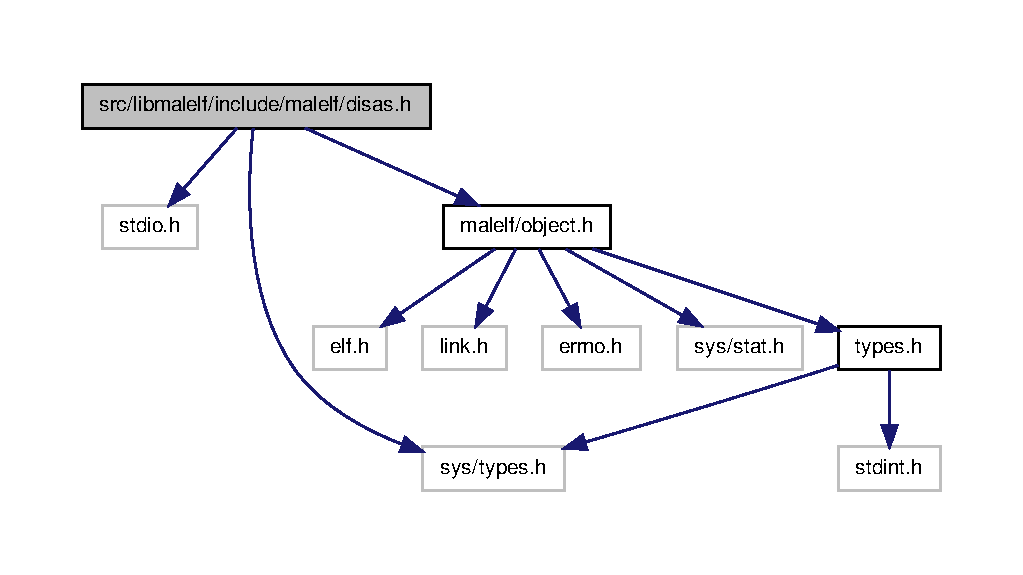
\includegraphics[width=400pt]{disas_8h__incl}
\end{center}
\end{figure}
This graph shows which files directly or indirectly include this file:\nopagebreak
\begin{figure}[H]
\begin{center}
\leavevmode
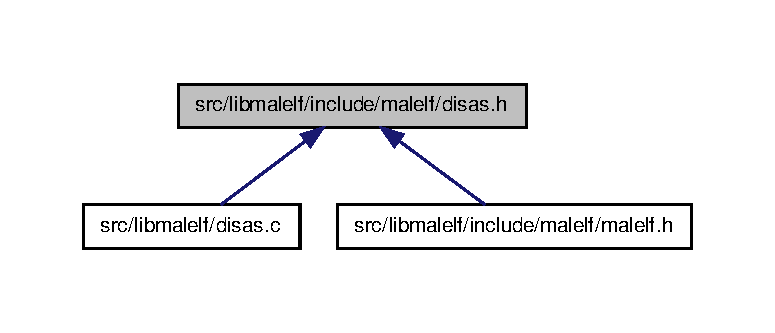
\includegraphics[width=372pt]{disas_8h__dep__incl}
\end{center}
\end{figure}
\subsection*{Functions}
\begin{DoxyCompactItemize}
\item 
\hyperlink{types_8h_aacb1ea6e27efde1c708a8bc4b56ee1a2}{\_\-i32} \hyperlink{disas_8h_aaed761394a2afd03b9e512cf14bdc95c}{malelf\_\-disas} (\hyperlink{structmalelf__object}{malelf\_\-object} $\ast$input, FILE $\ast$out)
\item 
\hyperlink{types_8h_aacb1ea6e27efde1c708a8bc4b56ee1a2}{\_\-i32} \hyperlink{disas_8h_ac49a05ddadb700e74b04d80b419e1054}{malelf\_\-disas\_\-section} (\hyperlink{structmalelf__object}{malelf\_\-object} $\ast$input, char $\ast$section, FILE $\ast$outfd)
\end{DoxyCompactItemize}


\subsection{Function Documentation}
\hypertarget{disas_8h_aaed761394a2afd03b9e512cf14bdc95c}{
\index{disas.h@{disas.h}!malelf\_\-disas@{malelf\_\-disas}}
\index{malelf\_\-disas@{malelf\_\-disas}!disas.h@{disas.h}}
\subsubsection[{malelf\_\-disas}]{\setlength{\rightskip}{0pt plus 5cm}{\bf \_\-i32} malelf\_\-disas (
\begin{DoxyParamCaption}
\item[{{\bf malelf\_\-object} $\ast$}]{input, }
\item[{FILE $\ast$}]{out}
\end{DoxyParamCaption}
)}}
\label{disas_8h_aaed761394a2afd03b9e512cf14bdc95c}


Definition at line 288 of file disas.c.

\hypertarget{disas_8h_ac49a05ddadb700e74b04d80b419e1054}{
\index{disas.h@{disas.h}!malelf\_\-disas\_\-section@{malelf\_\-disas\_\-section}}
\index{malelf\_\-disas\_\-section@{malelf\_\-disas\_\-section}!disas.h@{disas.h}}
\subsubsection[{malelf\_\-disas\_\-section}]{\setlength{\rightskip}{0pt plus 5cm}{\bf \_\-i32} malelf\_\-disas\_\-section (
\begin{DoxyParamCaption}
\item[{{\bf malelf\_\-object} $\ast$}]{input, }
\item[{char $\ast$}]{section, }
\item[{FILE $\ast$}]{outfd}
\end{DoxyParamCaption}
)}}
\label{disas_8h_ac49a05ddadb700e74b04d80b419e1054}


Definition at line 226 of file disas.c.


\hypertarget{dissect_8h}{
\section{src/libmalelf/include/malelf/dissect.h File Reference}
\label{dissect_8h}\index{src/libmalelf/include/malelf/dissect.h@{src/libmalelf/include/malelf/dissect.h}}
}
This graph shows which files directly or indirectly include this file:\nopagebreak
\begin{figure}[H]
\begin{center}
\leavevmode
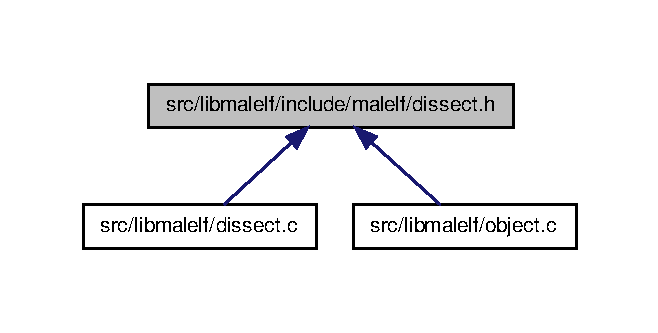
\includegraphics[width=316pt]{dissect_8h__dep__incl}
\end{center}
\end{figure}
\subsection*{Classes}
\begin{DoxyCompactItemize}
\item 
struct \hyperlink{structtb__column}{tb\_\-column}
\item 
struct \hyperlink{structtb__line}{tb\_\-line}
\end{DoxyCompactItemize}
\subsection*{Defines}
\begin{DoxyCompactItemize}
\item 
\#define \hyperlink{dissect_8h_a549e26b0208bdad59ec0d83d711dc018}{SET\_\-COLNAME}(col, str)~strncpy(col.name, str, 80); (col.size = 0)
\end{DoxyCompactItemize}
\subsection*{Typedefs}
\begin{DoxyCompactItemize}
\item 
typedef \hyperlink{structtb__line}{tb\_\-line} \hyperlink{dissect_8h_a0b1577938e3b6fd39373ffc431157ad5}{tb\_\-header}
\item 
typedef \hyperlink{structtb__line}{tb\_\-line} \hyperlink{dissect_8h_a9957462c6e60c222284c883663df3c47}{tb\_\-generic\_\-line}
\end{DoxyCompactItemize}
\subsection*{Functions}
\begin{DoxyCompactItemize}
\item 
void \hyperlink{dissect_8h_a91d724e17c03d2e4e3f5a0cecd4a496a}{print\_\-table\_\-generic} (\hyperlink{structtb__line}{tb\_\-line} $\ast$, int, int, int)
\item 
void \hyperlink{dissect_8h_ad666266f8e36f9f7718af128f545d7a8}{print\_\-table\_\-line} (\hyperlink{structtb__line}{tb\_\-line} $\ast$, int, int)
\item 
void \hyperlink{dissect_8h_a0eb2aa8e2bd01a36f18b8874f07c6be3}{print\_\-table\_\-header} (\hyperlink{structtb__line}{tb\_\-header} $\ast$, int, int)
\item 
void \hyperlink{dissect_8h_aec6ee2c7cfaccd010e6e6f433fd5938e}{print\_\-table\_\-header\_\-art} (int, int)
\item 
\hyperlink{types_8h_aacb1ea6e27efde1c708a8bc4b56ee1a2}{\_\-i32} \hyperlink{dissect_8h_a6fad0db775504c32cd2bbdbb984902ce}{malelf\_\-sections\_\-exec} (\hyperlink{structmalelf__object}{malelf\_\-object} $\ast$elf\_\-obj, \hyperlink{types_8h_aacb1ea6e27efde1c708a8bc4b56ee1a2}{\_\-i32}($\ast$callback)(char $\ast$sect\_\-n, char $\ast$sect\_\-t, void $\ast$arg), void $\ast$arg)
\end{DoxyCompactItemize}


\subsection{Define Documentation}
\hypertarget{dissect_8h_a549e26b0208bdad59ec0d83d711dc018}{
\index{dissect.h@{dissect.h}!SET\_\-COLNAME@{SET\_\-COLNAME}}
\index{SET\_\-COLNAME@{SET\_\-COLNAME}!dissect.h@{dissect.h}}
\subsubsection[{SET\_\-COLNAME}]{\setlength{\rightskip}{0pt plus 5cm}\#define SET\_\-COLNAME(
\begin{DoxyParamCaption}
\item[{}]{col, }
\item[{}]{str}
\end{DoxyParamCaption}
)~strncpy(col.name, str, 80); (col.size = 0)}}
\label{dissect_8h_a549e26b0208bdad59ec0d83d711dc018}


Definition at line 17 of file dissect.h.



\subsection{Typedef Documentation}
\hypertarget{dissect_8h_a9957462c6e60c222284c883663df3c47}{
\index{dissect.h@{dissect.h}!tb\_\-generic\_\-line@{tb\_\-generic\_\-line}}
\index{tb\_\-generic\_\-line@{tb\_\-generic\_\-line}!dissect.h@{dissect.h}}
\subsubsection[{tb\_\-generic\_\-line}]{\setlength{\rightskip}{0pt plus 5cm}typedef {\bf tb\_\-line} {\bf tb\_\-generic\_\-line}}}
\label{dissect_8h_a9957462c6e60c222284c883663df3c47}


Definition at line 15 of file dissect.h.

\hypertarget{dissect_8h_a0b1577938e3b6fd39373ffc431157ad5}{
\index{dissect.h@{dissect.h}!tb\_\-header@{tb\_\-header}}
\index{tb\_\-header@{tb\_\-header}!dissect.h@{dissect.h}}
\subsubsection[{tb\_\-header}]{\setlength{\rightskip}{0pt plus 5cm}typedef {\bf tb\_\-line} {\bf tb\_\-header}}}
\label{dissect_8h_a0b1577938e3b6fd39373ffc431157ad5}


Definition at line 14 of file dissect.h.



\subsection{Function Documentation}
\hypertarget{dissect_8h_a6fad0db775504c32cd2bbdbb984902ce}{
\index{dissect.h@{dissect.h}!malelf\_\-sections\_\-exec@{malelf\_\-sections\_\-exec}}
\index{malelf\_\-sections\_\-exec@{malelf\_\-sections\_\-exec}!dissect.h@{dissect.h}}
\subsubsection[{malelf\_\-sections\_\-exec}]{\setlength{\rightskip}{0pt plus 5cm}{\bf \_\-i32} malelf\_\-sections\_\-exec (
\begin{DoxyParamCaption}
\item[{{\bf malelf\_\-object} $\ast$}]{elf\_\-obj, }
\item[{{\bf \_\-i32}($\ast$)(char $\ast$sect\_\-n, char $\ast$sect\_\-t, void $\ast$arg)}]{callback, }
\item[{void $\ast$}]{arg}
\end{DoxyParamCaption}
)}}
\label{dissect_8h_a6fad0db775504c32cd2bbdbb984902ce}


Definition at line 14 of file dissect.c.

\hypertarget{dissect_8h_a91d724e17c03d2e4e3f5a0cecd4a496a}{
\index{dissect.h@{dissect.h}!print\_\-table\_\-generic@{print\_\-table\_\-generic}}
\index{print\_\-table\_\-generic@{print\_\-table\_\-generic}!dissect.h@{dissect.h}}
\subsubsection[{print\_\-table\_\-generic}]{\setlength{\rightskip}{0pt plus 5cm}void print\_\-table\_\-generic (
\begin{DoxyParamCaption}
\item[{{\bf tb\_\-line} $\ast$}]{, }
\item[{int}]{, }
\item[{int}]{, }
\item[{int}]{}
\end{DoxyParamCaption}
)}}
\label{dissect_8h_a91d724e17c03d2e4e3f5a0cecd4a496a}
\hypertarget{dissect_8h_a0eb2aa8e2bd01a36f18b8874f07c6be3}{
\index{dissect.h@{dissect.h}!print\_\-table\_\-header@{print\_\-table\_\-header}}
\index{print\_\-table\_\-header@{print\_\-table\_\-header}!dissect.h@{dissect.h}}
\subsubsection[{print\_\-table\_\-header}]{\setlength{\rightskip}{0pt plus 5cm}void print\_\-table\_\-header (
\begin{DoxyParamCaption}
\item[{{\bf tb\_\-header} $\ast$}]{, }
\item[{int}]{, }
\item[{int}]{}
\end{DoxyParamCaption}
)}}
\label{dissect_8h_a0eb2aa8e2bd01a36f18b8874f07c6be3}


Definition at line 137 of file print\_\-table.c.

\hypertarget{dissect_8h_aec6ee2c7cfaccd010e6e6f433fd5938e}{
\index{dissect.h@{dissect.h}!print\_\-table\_\-header\_\-art@{print\_\-table\_\-header\_\-art}}
\index{print\_\-table\_\-header\_\-art@{print\_\-table\_\-header\_\-art}!dissect.h@{dissect.h}}
\subsubsection[{print\_\-table\_\-header\_\-art}]{\setlength{\rightskip}{0pt plus 5cm}void print\_\-table\_\-header\_\-art (
\begin{DoxyParamCaption}
\item[{int}]{, }
\item[{int}]{}
\end{DoxyParamCaption}
)}}
\label{dissect_8h_aec6ee2c7cfaccd010e6e6f433fd5938e}


Definition at line 145 of file print\_\-table.c.

\hypertarget{dissect_8h_ad666266f8e36f9f7718af128f545d7a8}{
\index{dissect.h@{dissect.h}!print\_\-table\_\-line@{print\_\-table\_\-line}}
\index{print\_\-table\_\-line@{print\_\-table\_\-line}!dissect.h@{dissect.h}}
\subsubsection[{print\_\-table\_\-line}]{\setlength{\rightskip}{0pt plus 5cm}void print\_\-table\_\-line (
\begin{DoxyParamCaption}
\item[{{\bf tb\_\-line} $\ast$}]{, }
\item[{int}]{, }
\item[{int}]{}
\end{DoxyParamCaption}
)}}
\label{dissect_8h_ad666266f8e36f9f7718af128f545d7a8}


Definition at line 141 of file print\_\-table.c.


\hypertarget{error_8h}{
\section{src/libmalelf/include/malelf/error.h File Reference}
\label{error_8h}\index{src/libmalelf/include/malelf/error.h@{src/libmalelf/include/malelf/error.h}}
}
{\ttfamily \#include \char`\"{}util.h\char`\"{}}\par
Include dependency graph for error.h:\nopagebreak
\begin{figure}[H]
\begin{center}
\leavevmode
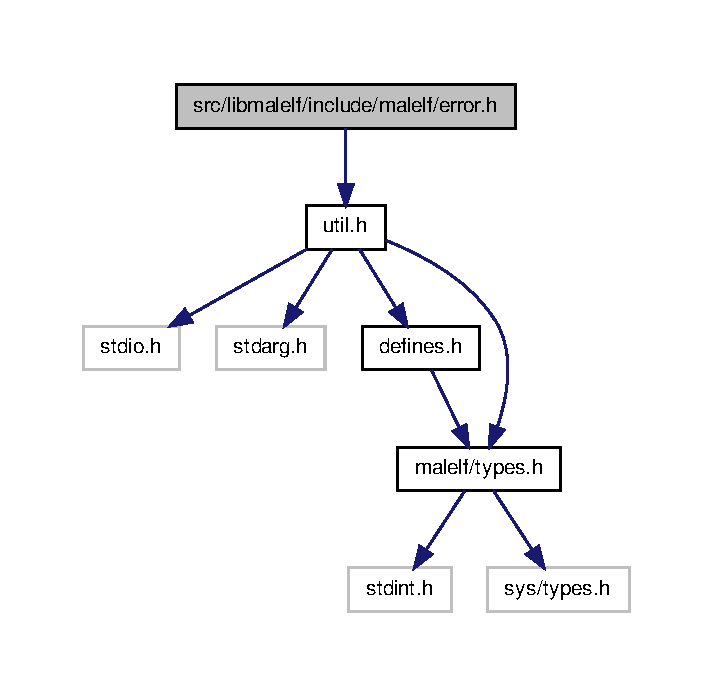
\includegraphics[width=342pt]{error_8h__incl}
\end{center}
\end{figure}
This graph shows which files directly or indirectly include this file:\nopagebreak
\begin{figure}[H]
\begin{center}
\leavevmode
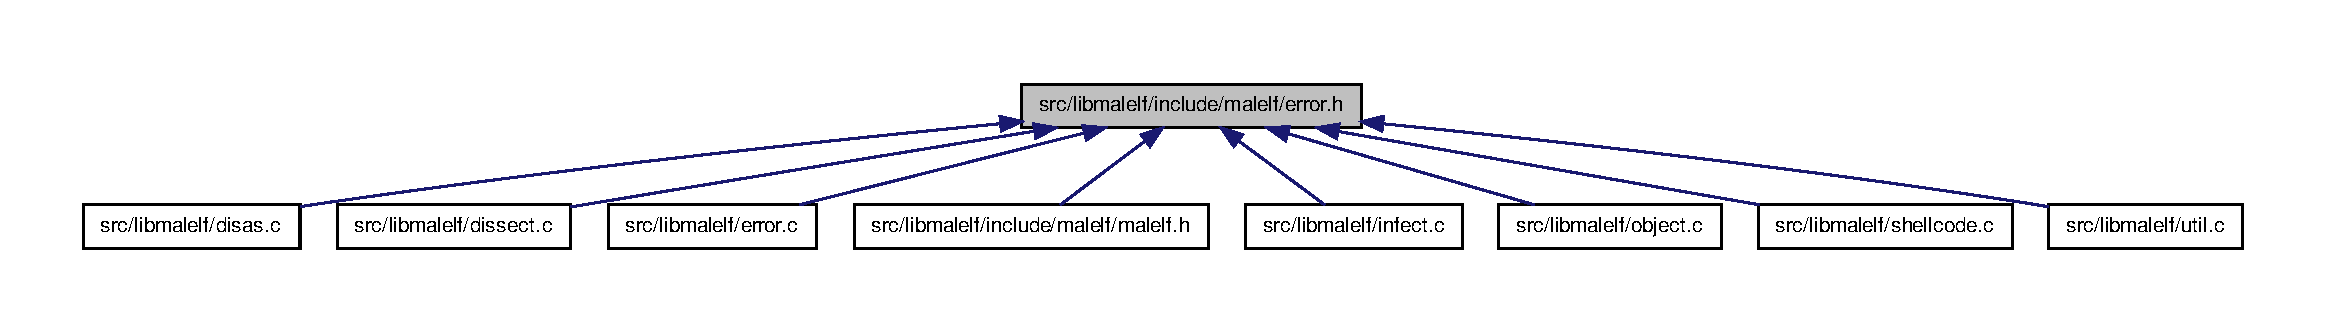
\includegraphics[width=400pt]{error_8h__dep__incl}
\end{center}
\end{figure}
\subsection*{Defines}
\begin{DoxyCompactItemize}
\item 
\#define \hyperlink{error_8h_afce77b261af529ab2d27aede030e3d5d}{MAX\_\-MSG\_\-ERROR}~255
\item 
\#define \hyperlink{error_8h_adcb6e8221db334cb7abe5a95a69be738}{malelf\_\-perror}(code)~\_\-malelf\_\-perror(code, \_\-\_\-FUNCTION\_\-\_\-, \_\-\_\-FILE\_\-\_\-, \_\-\_\-LINE\_\-\_\-)
\item 
\#define \hyperlink{error_8h_a218041a27ba26b07e91ed8b9628e1175}{malelf\_\-fatal}(code)~do \{malelf\_\-perror(code); LOG\_\-ERROR(\char`\"{}Aborting...$\backslash$n\char`\"{}); exit(code); \} while(0)
\end{DoxyCompactItemize}
\subsection*{Enumerations}
\begin{DoxyCompactItemize}
\item 
enum \hyperlink{error_8h_abd29c481acbfdbb1e3a130f584cd8396}{malelf\_\-status} \{ \par
\hyperlink{error_8h_abd29c481acbfdbb1e3a130f584cd8396a38930d6cba46e530d1e66073b5de69e5}{MALELF\_\-SUCCESS} =  0, 
\hyperlink{error_8h_abd29c481acbfdbb1e3a130f584cd8396aad0c08e49defceac643bb4f9988d9f8f}{MALELF\_\-EPERM}, 
\hyperlink{error_8h_abd29c481acbfdbb1e3a130f584cd8396a5f45b921e06c13ee5b738ffb0c209296}{MALELF\_\-ENOENT} =  2, 
\hyperlink{error_8h_abd29c481acbfdbb1e3a130f584cd8396a7c867d113b85c9c1870b4d203518b8cf}{MALELF\_\-ESRCH} =  3, 
\par
\hyperlink{error_8h_abd29c481acbfdbb1e3a130f584cd8396a2b6f3afc3b2fe630fcff3f2a46ba5919}{MALELF\_\-EINTR} =  4, 
\hyperlink{error_8h_abd29c481acbfdbb1e3a130f584cd8396a2ebc3eaf7ef60e29312f76c2cb17de15}{MALELF\_\-EIO} =  5, 
\hyperlink{error_8h_abd29c481acbfdbb1e3a130f584cd8396aa611099f72230193f83a8c9c193ddc23}{MALELF\_\-ENXIO} =  6, 
\hyperlink{error_8h_abd29c481acbfdbb1e3a130f584cd8396a40292197fbfa2fb768734bf9c54d9229}{MALELF\_\-E2BIG} =  7, 
\par
\hyperlink{error_8h_abd29c481acbfdbb1e3a130f584cd8396a37b69ef863d181f9f544b453c43e72a4}{MALELF\_\-ENOEXEC} =  8, 
\hyperlink{error_8h_abd29c481acbfdbb1e3a130f584cd8396a1fcb2c524e8b39b67d168f336ebcf80f}{MALELF\_\-EBADF} =  9, 
\hyperlink{error_8h_abd29c481acbfdbb1e3a130f584cd8396a9d50af435c11e43ea4377f9eb01cfa86}{MALELF\_\-ECHILD} =  10, 
\hyperlink{error_8h_abd29c481acbfdbb1e3a130f584cd8396adf96f48a66644f27844648b20efe732e}{MALELF\_\-EAGAIN} =  11, 
\par
\hyperlink{error_8h_abd29c481acbfdbb1e3a130f584cd8396af3340308d4a4f286b5b54f46f57dc6c7}{MALELF\_\-ENOMEM} =  12, 
\hyperlink{error_8h_abd29c481acbfdbb1e3a130f584cd8396ab4722ff1f97425d6d698e5c9c10585c0}{MALELF\_\-EACCES} =  13, 
\hyperlink{error_8h_abd29c481acbfdbb1e3a130f584cd8396a90a15e744bde0fcfa1188ffbfaed5853}{MALELF\_\-EFAULT} =  14, 
\hyperlink{error_8h_abd29c481acbfdbb1e3a130f584cd8396a079897b63396ad30d1ead7594d5febcb}{MALELF\_\-ENOTBLK} =  15, 
\par
\hyperlink{error_8h_abd29c481acbfdbb1e3a130f584cd8396a75dd1a239a6945d146c894f5c69c227f}{MALELF\_\-EBUSY} =  16, 
\hyperlink{error_8h_abd29c481acbfdbb1e3a130f584cd8396a074b9914c84d76d46f8241bbd07e1342}{MALELF\_\-EEXIST} =  17, 
\hyperlink{error_8h_abd29c481acbfdbb1e3a130f584cd8396a3eda38632f4bc2f4d8ca1d77a349db31}{MALELF\_\-EXDEV} =  18, 
\hyperlink{error_8h_abd29c481acbfdbb1e3a130f584cd8396a437a5f035b19248ab1d38bcb0bc68218}{MALELF\_\-ENODEV} =  19, 
\par
\hyperlink{error_8h_abd29c481acbfdbb1e3a130f584cd8396a03318bef646591285e4d3b46951fd0cb}{MALELF\_\-ENOTDIR} =  20, 
\hyperlink{error_8h_abd29c481acbfdbb1e3a130f584cd8396ada956b7a01fb6a374b5d5d2d03f01dac}{MALELF\_\-EISDIR} =  21, 
\hyperlink{error_8h_abd29c481acbfdbb1e3a130f584cd8396a1476c342aa1e55fcb98a3affbbc153f3}{MALELF\_\-EINVAL} =  22, 
\hyperlink{error_8h_abd29c481acbfdbb1e3a130f584cd8396a5c8c81623f77ba3a8975a17b1b6f04c8}{MALELF\_\-ENFILE} =  23, 
\par
\hyperlink{error_8h_abd29c481acbfdbb1e3a130f584cd8396adb8a8c4338de65517e3a500cfa3c5b22}{MALELF\_\-EMFILE} =  24, 
\hyperlink{error_8h_abd29c481acbfdbb1e3a130f584cd8396aee7fd0d8e05ec541514afc0762bca6ef}{MALELF\_\-ENOTTY} =  25, 
\hyperlink{error_8h_abd29c481acbfdbb1e3a130f584cd8396a37c71f23d51e3fd49e7a7e56b2982cf6}{MALELF\_\-ETXTBSY} =  26, 
\hyperlink{error_8h_abd29c481acbfdbb1e3a130f584cd8396a97ec90cd4dac35b522766e270ca77d6c}{MALELF\_\-EFBIG} =  27, 
\par
\hyperlink{error_8h_abd29c481acbfdbb1e3a130f584cd8396adc82412258b84334ffdede147c60333f}{MALELF\_\-ENOSPC} =  28, 
\hyperlink{error_8h_abd29c481acbfdbb1e3a130f584cd8396a065351079e4e5c6516e97f50919faf4f}{MALELF\_\-ESPIPE} =  29, 
\hyperlink{error_8h_abd29c481acbfdbb1e3a130f584cd8396a880c50d78649d8cd12dd8603d535668e}{MALELF\_\-EROFS} =  30, 
\hyperlink{error_8h_abd29c481acbfdbb1e3a130f584cd8396abecdfa6cbdd9e7bb33fee5009198520f}{MALELF\_\-EMLINK} =  31, 
\par
\hyperlink{error_8h_abd29c481acbfdbb1e3a130f584cd8396ab5ca45afa1e06d9794ba8954effba1d5}{MALELF\_\-EPIPE} =  32, 
\hyperlink{error_8h_abd29c481acbfdbb1e3a130f584cd8396a0c2471fb978bb3ad6d2e1d7e2f94f864}{MALELF\_\-EDOM} =  33, 
\hyperlink{error_8h_abd29c481acbfdbb1e3a130f584cd8396a6abe58feecf46f632bc60024751c54f2}{MALELF\_\-ERANGE} =  34, 
\hyperlink{error_8h_abd29c481acbfdbb1e3a130f584cd8396acc31e1d217a7c3609d0957fda7a60091}{MALELF\_\-LAST\_\-ERRNO} =  35, 
\par
\hyperlink{error_8h_abd29c481acbfdbb1e3a130f584cd8396af38b955564dfc1ad5b66a92ce9605292}{MALELF\_\-ERROR} =  40, 
\hyperlink{error_8h_abd29c481acbfdbb1e3a130f584cd8396a4874e35f449f940637ae57c7df768819}{MALELF\_\-ECLOSED} =  41, 
\hyperlink{error_8h_abd29c481acbfdbb1e3a130f584cd8396a2fd4b073eef0b92fee71d4dfcfdbf9e6}{MALELF\_\-EALLOC} =  42, 
\hyperlink{error_8h_abd29c481acbfdbb1e3a130f584cd8396ad720e04b4a6485f7399d181a261b8f34}{MALELF\_\-ENOT\_\-ELF} =  43, 
\par
\hyperlink{error_8h_abd29c481acbfdbb1e3a130f584cd8396a1ef947cc4e5195824c2b2d0f8e100d59}{MALELF\_\-ECORRUPTED} =  44, 
\hyperlink{error_8h_abd29c481acbfdbb1e3a130f584cd8396a6b303b728d27224f4f240e49c81f01f4}{MALELF\_\-ESUSPECT\_\-SECTIONS} =  45, 
\hyperlink{error_8h_abd29c481acbfdbb1e3a130f584cd8396a709012064bf03c5cef267cecd22c704a}{MALELF\_\-EMISSING\_\-MAGIC\_\-BYTES} =  46, 
\hyperlink{error_8h_abd29c481acbfdbb1e3a130f584cd8396ac08109e3a94a13028d8281d2a22a20a5}{MALELF\_\-EINV\_\-OFFSET\_\-ENTRY} =  47, 
\par
\hyperlink{error_8h_abd29c481acbfdbb1e3a130f584cd8396a210321970e70f26186c9470910e0ecc9}{MALELF\_\-EDISAS} =  48, 
\hyperlink{error_8h_abd29c481acbfdbb1e3a130f584cd8396a90d553dba8b6c0969af7f0776fed67d0}{MALELF\_\-LAST\_\-ERROR} =  50
 \}
\end{DoxyCompactItemize}
\subsection*{Functions}
\begin{DoxyCompactItemize}
\item 
void \hyperlink{error_8h_ad60f880160e465f8f99c9d4ad8c95d21}{\_\-malelf\_\-perror} (int code, const char $\ast$func, const char $\ast$file, int line)
\item 
const char $\ast$ \hyperlink{error_8h_af225ce01f3f2709e264c7036e813c3b1}{malelf\_\-strerror} (int code)
\end{DoxyCompactItemize}


\subsection{Define Documentation}
\hypertarget{error_8h_a218041a27ba26b07e91ed8b9628e1175}{
\index{error.h@{error.h}!malelf\_\-fatal@{malelf\_\-fatal}}
\index{malelf\_\-fatal@{malelf\_\-fatal}!error.h@{error.h}}
\subsubsection[{malelf\_\-fatal}]{\setlength{\rightskip}{0pt plus 5cm}\#define malelf\_\-fatal(
\begin{DoxyParamCaption}
\item[{}]{code}
\end{DoxyParamCaption}
)~do \{malelf\_\-perror(code); LOG\_\-ERROR(\char`\"{}Aborting...$\backslash$n\char`\"{}); exit(code); \} while(0)}}
\label{error_8h_a218041a27ba26b07e91ed8b9628e1175}


Definition at line 60 of file error.h.

\hypertarget{error_8h_adcb6e8221db334cb7abe5a95a69be738}{
\index{error.h@{error.h}!malelf\_\-perror@{malelf\_\-perror}}
\index{malelf\_\-perror@{malelf\_\-perror}!error.h@{error.h}}
\subsubsection[{malelf\_\-perror}]{\setlength{\rightskip}{0pt plus 5cm}\#define malelf\_\-perror(
\begin{DoxyParamCaption}
\item[{}]{code}
\end{DoxyParamCaption}
)~\_\-malelf\_\-perror(code, \_\-\_\-FUNCTION\_\-\_\-, \_\-\_\-FILE\_\-\_\-, \_\-\_\-LINE\_\-\_\-)}}
\label{error_8h_adcb6e8221db334cb7abe5a95a69be738}


Definition at line 59 of file error.h.

\hypertarget{error_8h_afce77b261af529ab2d27aede030e3d5d}{
\index{error.h@{error.h}!MAX\_\-MSG\_\-ERROR@{MAX\_\-MSG\_\-ERROR}}
\index{MAX\_\-MSG\_\-ERROR@{MAX\_\-MSG\_\-ERROR}!error.h@{error.h}}
\subsubsection[{MAX\_\-MSG\_\-ERROR}]{\setlength{\rightskip}{0pt plus 5cm}\#define MAX\_\-MSG\_\-ERROR~255}}
\label{error_8h_afce77b261af529ab2d27aede030e3d5d}


Definition at line 6 of file error.h.



\subsection{Enumeration Type Documentation}
\hypertarget{error_8h_abd29c481acbfdbb1e3a130f584cd8396}{
\index{error.h@{error.h}!malelf\_\-status@{malelf\_\-status}}
\index{malelf\_\-status@{malelf\_\-status}!error.h@{error.h}}
\subsubsection[{malelf\_\-status}]{\setlength{\rightskip}{0pt plus 5cm}enum {\bf malelf\_\-status}}}
\label{error_8h_abd29c481acbfdbb1e3a130f584cd8396}
\begin{Desc}
\item[Enumerator: ]\par
\begin{description}
\index{MALELF\_\-SUCCESS@{MALELF\_\-SUCCESS}!error.h@{error.h}}\index{error.h@{error.h}!MALELF\_\-SUCCESS@{MALELF\_\-SUCCESS}}\item[{\em 
\hypertarget{error_8h_abd29c481acbfdbb1e3a130f584cd8396a38930d6cba46e530d1e66073b5de69e5}{
MALELF\_\-SUCCESS}
\label{error_8h_abd29c481acbfdbb1e3a130f584cd8396a38930d6cba46e530d1e66073b5de69e5}
}]\index{MALELF\_\-EPERM@{MALELF\_\-EPERM}!error.h@{error.h}}\index{error.h@{error.h}!MALELF\_\-EPERM@{MALELF\_\-EPERM}}\item[{\em 
\hypertarget{error_8h_abd29c481acbfdbb1e3a130f584cd8396aad0c08e49defceac643bb4f9988d9f8f}{
MALELF\_\-EPERM}
\label{error_8h_abd29c481acbfdbb1e3a130f584cd8396aad0c08e49defceac643bb4f9988d9f8f}
}]\index{MALELF\_\-ENOENT@{MALELF\_\-ENOENT}!error.h@{error.h}}\index{error.h@{error.h}!MALELF\_\-ENOENT@{MALELF\_\-ENOENT}}\item[{\em 
\hypertarget{error_8h_abd29c481acbfdbb1e3a130f584cd8396a5f45b921e06c13ee5b738ffb0c209296}{
MALELF\_\-ENOENT}
\label{error_8h_abd29c481acbfdbb1e3a130f584cd8396a5f45b921e06c13ee5b738ffb0c209296}
}]\index{MALELF\_\-ESRCH@{MALELF\_\-ESRCH}!error.h@{error.h}}\index{error.h@{error.h}!MALELF\_\-ESRCH@{MALELF\_\-ESRCH}}\item[{\em 
\hypertarget{error_8h_abd29c481acbfdbb1e3a130f584cd8396a7c867d113b85c9c1870b4d203518b8cf}{
MALELF\_\-ESRCH}
\label{error_8h_abd29c481acbfdbb1e3a130f584cd8396a7c867d113b85c9c1870b4d203518b8cf}
}]\index{MALELF\_\-EINTR@{MALELF\_\-EINTR}!error.h@{error.h}}\index{error.h@{error.h}!MALELF\_\-EINTR@{MALELF\_\-EINTR}}\item[{\em 
\hypertarget{error_8h_abd29c481acbfdbb1e3a130f584cd8396a2b6f3afc3b2fe630fcff3f2a46ba5919}{
MALELF\_\-EINTR}
\label{error_8h_abd29c481acbfdbb1e3a130f584cd8396a2b6f3afc3b2fe630fcff3f2a46ba5919}
}]\index{MALELF\_\-EIO@{MALELF\_\-EIO}!error.h@{error.h}}\index{error.h@{error.h}!MALELF\_\-EIO@{MALELF\_\-EIO}}\item[{\em 
\hypertarget{error_8h_abd29c481acbfdbb1e3a130f584cd8396a2ebc3eaf7ef60e29312f76c2cb17de15}{
MALELF\_\-EIO}
\label{error_8h_abd29c481acbfdbb1e3a130f584cd8396a2ebc3eaf7ef60e29312f76c2cb17de15}
}]\index{MALELF\_\-ENXIO@{MALELF\_\-ENXIO}!error.h@{error.h}}\index{error.h@{error.h}!MALELF\_\-ENXIO@{MALELF\_\-ENXIO}}\item[{\em 
\hypertarget{error_8h_abd29c481acbfdbb1e3a130f584cd8396aa611099f72230193f83a8c9c193ddc23}{
MALELF\_\-ENXIO}
\label{error_8h_abd29c481acbfdbb1e3a130f584cd8396aa611099f72230193f83a8c9c193ddc23}
}]\index{MALELF\_\-E2BIG@{MALELF\_\-E2BIG}!error.h@{error.h}}\index{error.h@{error.h}!MALELF\_\-E2BIG@{MALELF\_\-E2BIG}}\item[{\em 
\hypertarget{error_8h_abd29c481acbfdbb1e3a130f584cd8396a40292197fbfa2fb768734bf9c54d9229}{
MALELF\_\-E2BIG}
\label{error_8h_abd29c481acbfdbb1e3a130f584cd8396a40292197fbfa2fb768734bf9c54d9229}
}]\index{MALELF\_\-ENOEXEC@{MALELF\_\-ENOEXEC}!error.h@{error.h}}\index{error.h@{error.h}!MALELF\_\-ENOEXEC@{MALELF\_\-ENOEXEC}}\item[{\em 
\hypertarget{error_8h_abd29c481acbfdbb1e3a130f584cd8396a37b69ef863d181f9f544b453c43e72a4}{
MALELF\_\-ENOEXEC}
\label{error_8h_abd29c481acbfdbb1e3a130f584cd8396a37b69ef863d181f9f544b453c43e72a4}
}]\index{MALELF\_\-EBADF@{MALELF\_\-EBADF}!error.h@{error.h}}\index{error.h@{error.h}!MALELF\_\-EBADF@{MALELF\_\-EBADF}}\item[{\em 
\hypertarget{error_8h_abd29c481acbfdbb1e3a130f584cd8396a1fcb2c524e8b39b67d168f336ebcf80f}{
MALELF\_\-EBADF}
\label{error_8h_abd29c481acbfdbb1e3a130f584cd8396a1fcb2c524e8b39b67d168f336ebcf80f}
}]\index{MALELF\_\-ECHILD@{MALELF\_\-ECHILD}!error.h@{error.h}}\index{error.h@{error.h}!MALELF\_\-ECHILD@{MALELF\_\-ECHILD}}\item[{\em 
\hypertarget{error_8h_abd29c481acbfdbb1e3a130f584cd8396a9d50af435c11e43ea4377f9eb01cfa86}{
MALELF\_\-ECHILD}
\label{error_8h_abd29c481acbfdbb1e3a130f584cd8396a9d50af435c11e43ea4377f9eb01cfa86}
}]\index{MALELF\_\-EAGAIN@{MALELF\_\-EAGAIN}!error.h@{error.h}}\index{error.h@{error.h}!MALELF\_\-EAGAIN@{MALELF\_\-EAGAIN}}\item[{\em 
\hypertarget{error_8h_abd29c481acbfdbb1e3a130f584cd8396adf96f48a66644f27844648b20efe732e}{
MALELF\_\-EAGAIN}
\label{error_8h_abd29c481acbfdbb1e3a130f584cd8396adf96f48a66644f27844648b20efe732e}
}]\index{MALELF\_\-ENOMEM@{MALELF\_\-ENOMEM}!error.h@{error.h}}\index{error.h@{error.h}!MALELF\_\-ENOMEM@{MALELF\_\-ENOMEM}}\item[{\em 
\hypertarget{error_8h_abd29c481acbfdbb1e3a130f584cd8396af3340308d4a4f286b5b54f46f57dc6c7}{
MALELF\_\-ENOMEM}
\label{error_8h_abd29c481acbfdbb1e3a130f584cd8396af3340308d4a4f286b5b54f46f57dc6c7}
}]\index{MALELF\_\-EACCES@{MALELF\_\-EACCES}!error.h@{error.h}}\index{error.h@{error.h}!MALELF\_\-EACCES@{MALELF\_\-EACCES}}\item[{\em 
\hypertarget{error_8h_abd29c481acbfdbb1e3a130f584cd8396ab4722ff1f97425d6d698e5c9c10585c0}{
MALELF\_\-EACCES}
\label{error_8h_abd29c481acbfdbb1e3a130f584cd8396ab4722ff1f97425d6d698e5c9c10585c0}
}]\index{MALELF\_\-EFAULT@{MALELF\_\-EFAULT}!error.h@{error.h}}\index{error.h@{error.h}!MALELF\_\-EFAULT@{MALELF\_\-EFAULT}}\item[{\em 
\hypertarget{error_8h_abd29c481acbfdbb1e3a130f584cd8396a90a15e744bde0fcfa1188ffbfaed5853}{
MALELF\_\-EFAULT}
\label{error_8h_abd29c481acbfdbb1e3a130f584cd8396a90a15e744bde0fcfa1188ffbfaed5853}
}]\index{MALELF\_\-ENOTBLK@{MALELF\_\-ENOTBLK}!error.h@{error.h}}\index{error.h@{error.h}!MALELF\_\-ENOTBLK@{MALELF\_\-ENOTBLK}}\item[{\em 
\hypertarget{error_8h_abd29c481acbfdbb1e3a130f584cd8396a079897b63396ad30d1ead7594d5febcb}{
MALELF\_\-ENOTBLK}
\label{error_8h_abd29c481acbfdbb1e3a130f584cd8396a079897b63396ad30d1ead7594d5febcb}
}]\index{MALELF\_\-EBUSY@{MALELF\_\-EBUSY}!error.h@{error.h}}\index{error.h@{error.h}!MALELF\_\-EBUSY@{MALELF\_\-EBUSY}}\item[{\em 
\hypertarget{error_8h_abd29c481acbfdbb1e3a130f584cd8396a75dd1a239a6945d146c894f5c69c227f}{
MALELF\_\-EBUSY}
\label{error_8h_abd29c481acbfdbb1e3a130f584cd8396a75dd1a239a6945d146c894f5c69c227f}
}]\index{MALELF\_\-EEXIST@{MALELF\_\-EEXIST}!error.h@{error.h}}\index{error.h@{error.h}!MALELF\_\-EEXIST@{MALELF\_\-EEXIST}}\item[{\em 
\hypertarget{error_8h_abd29c481acbfdbb1e3a130f584cd8396a074b9914c84d76d46f8241bbd07e1342}{
MALELF\_\-EEXIST}
\label{error_8h_abd29c481acbfdbb1e3a130f584cd8396a074b9914c84d76d46f8241bbd07e1342}
}]\index{MALELF\_\-EXDEV@{MALELF\_\-EXDEV}!error.h@{error.h}}\index{error.h@{error.h}!MALELF\_\-EXDEV@{MALELF\_\-EXDEV}}\item[{\em 
\hypertarget{error_8h_abd29c481acbfdbb1e3a130f584cd8396a3eda38632f4bc2f4d8ca1d77a349db31}{
MALELF\_\-EXDEV}
\label{error_8h_abd29c481acbfdbb1e3a130f584cd8396a3eda38632f4bc2f4d8ca1d77a349db31}
}]\index{MALELF\_\-ENODEV@{MALELF\_\-ENODEV}!error.h@{error.h}}\index{error.h@{error.h}!MALELF\_\-ENODEV@{MALELF\_\-ENODEV}}\item[{\em 
\hypertarget{error_8h_abd29c481acbfdbb1e3a130f584cd8396a437a5f035b19248ab1d38bcb0bc68218}{
MALELF\_\-ENODEV}
\label{error_8h_abd29c481acbfdbb1e3a130f584cd8396a437a5f035b19248ab1d38bcb0bc68218}
}]\index{MALELF\_\-ENOTDIR@{MALELF\_\-ENOTDIR}!error.h@{error.h}}\index{error.h@{error.h}!MALELF\_\-ENOTDIR@{MALELF\_\-ENOTDIR}}\item[{\em 
\hypertarget{error_8h_abd29c481acbfdbb1e3a130f584cd8396a03318bef646591285e4d3b46951fd0cb}{
MALELF\_\-ENOTDIR}
\label{error_8h_abd29c481acbfdbb1e3a130f584cd8396a03318bef646591285e4d3b46951fd0cb}
}]\index{MALELF\_\-EISDIR@{MALELF\_\-EISDIR}!error.h@{error.h}}\index{error.h@{error.h}!MALELF\_\-EISDIR@{MALELF\_\-EISDIR}}\item[{\em 
\hypertarget{error_8h_abd29c481acbfdbb1e3a130f584cd8396ada956b7a01fb6a374b5d5d2d03f01dac}{
MALELF\_\-EISDIR}
\label{error_8h_abd29c481acbfdbb1e3a130f584cd8396ada956b7a01fb6a374b5d5d2d03f01dac}
}]\index{MALELF\_\-EINVAL@{MALELF\_\-EINVAL}!error.h@{error.h}}\index{error.h@{error.h}!MALELF\_\-EINVAL@{MALELF\_\-EINVAL}}\item[{\em 
\hypertarget{error_8h_abd29c481acbfdbb1e3a130f584cd8396a1476c342aa1e55fcb98a3affbbc153f3}{
MALELF\_\-EINVAL}
\label{error_8h_abd29c481acbfdbb1e3a130f584cd8396a1476c342aa1e55fcb98a3affbbc153f3}
}]\index{MALELF\_\-ENFILE@{MALELF\_\-ENFILE}!error.h@{error.h}}\index{error.h@{error.h}!MALELF\_\-ENFILE@{MALELF\_\-ENFILE}}\item[{\em 
\hypertarget{error_8h_abd29c481acbfdbb1e3a130f584cd8396a5c8c81623f77ba3a8975a17b1b6f04c8}{
MALELF\_\-ENFILE}
\label{error_8h_abd29c481acbfdbb1e3a130f584cd8396a5c8c81623f77ba3a8975a17b1b6f04c8}
}]\index{MALELF\_\-EMFILE@{MALELF\_\-EMFILE}!error.h@{error.h}}\index{error.h@{error.h}!MALELF\_\-EMFILE@{MALELF\_\-EMFILE}}\item[{\em 
\hypertarget{error_8h_abd29c481acbfdbb1e3a130f584cd8396adb8a8c4338de65517e3a500cfa3c5b22}{
MALELF\_\-EMFILE}
\label{error_8h_abd29c481acbfdbb1e3a130f584cd8396adb8a8c4338de65517e3a500cfa3c5b22}
}]\index{MALELF\_\-ENOTTY@{MALELF\_\-ENOTTY}!error.h@{error.h}}\index{error.h@{error.h}!MALELF\_\-ENOTTY@{MALELF\_\-ENOTTY}}\item[{\em 
\hypertarget{error_8h_abd29c481acbfdbb1e3a130f584cd8396aee7fd0d8e05ec541514afc0762bca6ef}{
MALELF\_\-ENOTTY}
\label{error_8h_abd29c481acbfdbb1e3a130f584cd8396aee7fd0d8e05ec541514afc0762bca6ef}
}]\index{MALELF\_\-ETXTBSY@{MALELF\_\-ETXTBSY}!error.h@{error.h}}\index{error.h@{error.h}!MALELF\_\-ETXTBSY@{MALELF\_\-ETXTBSY}}\item[{\em 
\hypertarget{error_8h_abd29c481acbfdbb1e3a130f584cd8396a37c71f23d51e3fd49e7a7e56b2982cf6}{
MALELF\_\-ETXTBSY}
\label{error_8h_abd29c481acbfdbb1e3a130f584cd8396a37c71f23d51e3fd49e7a7e56b2982cf6}
}]\index{MALELF\_\-EFBIG@{MALELF\_\-EFBIG}!error.h@{error.h}}\index{error.h@{error.h}!MALELF\_\-EFBIG@{MALELF\_\-EFBIG}}\item[{\em 
\hypertarget{error_8h_abd29c481acbfdbb1e3a130f584cd8396a97ec90cd4dac35b522766e270ca77d6c}{
MALELF\_\-EFBIG}
\label{error_8h_abd29c481acbfdbb1e3a130f584cd8396a97ec90cd4dac35b522766e270ca77d6c}
}]\index{MALELF\_\-ENOSPC@{MALELF\_\-ENOSPC}!error.h@{error.h}}\index{error.h@{error.h}!MALELF\_\-ENOSPC@{MALELF\_\-ENOSPC}}\item[{\em 
\hypertarget{error_8h_abd29c481acbfdbb1e3a130f584cd8396adc82412258b84334ffdede147c60333f}{
MALELF\_\-ENOSPC}
\label{error_8h_abd29c481acbfdbb1e3a130f584cd8396adc82412258b84334ffdede147c60333f}
}]\index{MALELF\_\-ESPIPE@{MALELF\_\-ESPIPE}!error.h@{error.h}}\index{error.h@{error.h}!MALELF\_\-ESPIPE@{MALELF\_\-ESPIPE}}\item[{\em 
\hypertarget{error_8h_abd29c481acbfdbb1e3a130f584cd8396a065351079e4e5c6516e97f50919faf4f}{
MALELF\_\-ESPIPE}
\label{error_8h_abd29c481acbfdbb1e3a130f584cd8396a065351079e4e5c6516e97f50919faf4f}
}]\index{MALELF\_\-EROFS@{MALELF\_\-EROFS}!error.h@{error.h}}\index{error.h@{error.h}!MALELF\_\-EROFS@{MALELF\_\-EROFS}}\item[{\em 
\hypertarget{error_8h_abd29c481acbfdbb1e3a130f584cd8396a880c50d78649d8cd12dd8603d535668e}{
MALELF\_\-EROFS}
\label{error_8h_abd29c481acbfdbb1e3a130f584cd8396a880c50d78649d8cd12dd8603d535668e}
}]\index{MALELF\_\-EMLINK@{MALELF\_\-EMLINK}!error.h@{error.h}}\index{error.h@{error.h}!MALELF\_\-EMLINK@{MALELF\_\-EMLINK}}\item[{\em 
\hypertarget{error_8h_abd29c481acbfdbb1e3a130f584cd8396abecdfa6cbdd9e7bb33fee5009198520f}{
MALELF\_\-EMLINK}
\label{error_8h_abd29c481acbfdbb1e3a130f584cd8396abecdfa6cbdd9e7bb33fee5009198520f}
}]\index{MALELF\_\-EPIPE@{MALELF\_\-EPIPE}!error.h@{error.h}}\index{error.h@{error.h}!MALELF\_\-EPIPE@{MALELF\_\-EPIPE}}\item[{\em 
\hypertarget{error_8h_abd29c481acbfdbb1e3a130f584cd8396ab5ca45afa1e06d9794ba8954effba1d5}{
MALELF\_\-EPIPE}
\label{error_8h_abd29c481acbfdbb1e3a130f584cd8396ab5ca45afa1e06d9794ba8954effba1d5}
}]\index{MALELF\_\-EDOM@{MALELF\_\-EDOM}!error.h@{error.h}}\index{error.h@{error.h}!MALELF\_\-EDOM@{MALELF\_\-EDOM}}\item[{\em 
\hypertarget{error_8h_abd29c481acbfdbb1e3a130f584cd8396a0c2471fb978bb3ad6d2e1d7e2f94f864}{
MALELF\_\-EDOM}
\label{error_8h_abd29c481acbfdbb1e3a130f584cd8396a0c2471fb978bb3ad6d2e1d7e2f94f864}
}]\index{MALELF\_\-ERANGE@{MALELF\_\-ERANGE}!error.h@{error.h}}\index{error.h@{error.h}!MALELF\_\-ERANGE@{MALELF\_\-ERANGE}}\item[{\em 
\hypertarget{error_8h_abd29c481acbfdbb1e3a130f584cd8396a6abe58feecf46f632bc60024751c54f2}{
MALELF\_\-ERANGE}
\label{error_8h_abd29c481acbfdbb1e3a130f584cd8396a6abe58feecf46f632bc60024751c54f2}
}]\index{MALELF\_\-LAST\_\-ERRNO@{MALELF\_\-LAST\_\-ERRNO}!error.h@{error.h}}\index{error.h@{error.h}!MALELF\_\-LAST\_\-ERRNO@{MALELF\_\-LAST\_\-ERRNO}}\item[{\em 
\hypertarget{error_8h_abd29c481acbfdbb1e3a130f584cd8396acc31e1d217a7c3609d0957fda7a60091}{
MALELF\_\-LAST\_\-ERRNO}
\label{error_8h_abd29c481acbfdbb1e3a130f584cd8396acc31e1d217a7c3609d0957fda7a60091}
}]\index{MALELF\_\-ERROR@{MALELF\_\-ERROR}!error.h@{error.h}}\index{error.h@{error.h}!MALELF\_\-ERROR@{MALELF\_\-ERROR}}\item[{\em 
\hypertarget{error_8h_abd29c481acbfdbb1e3a130f584cd8396af38b955564dfc1ad5b66a92ce9605292}{
MALELF\_\-ERROR}
\label{error_8h_abd29c481acbfdbb1e3a130f584cd8396af38b955564dfc1ad5b66a92ce9605292}
}]\index{MALELF\_\-ECLOSED@{MALELF\_\-ECLOSED}!error.h@{error.h}}\index{error.h@{error.h}!MALELF\_\-ECLOSED@{MALELF\_\-ECLOSED}}\item[{\em 
\hypertarget{error_8h_abd29c481acbfdbb1e3a130f584cd8396a4874e35f449f940637ae57c7df768819}{
MALELF\_\-ECLOSED}
\label{error_8h_abd29c481acbfdbb1e3a130f584cd8396a4874e35f449f940637ae57c7df768819}
}]\index{MALELF\_\-EALLOC@{MALELF\_\-EALLOC}!error.h@{error.h}}\index{error.h@{error.h}!MALELF\_\-EALLOC@{MALELF\_\-EALLOC}}\item[{\em 
\hypertarget{error_8h_abd29c481acbfdbb1e3a130f584cd8396a2fd4b073eef0b92fee71d4dfcfdbf9e6}{
MALELF\_\-EALLOC}
\label{error_8h_abd29c481acbfdbb1e3a130f584cd8396a2fd4b073eef0b92fee71d4dfcfdbf9e6}
}]\index{MALELF\_\-ENOT\_\-ELF@{MALELF\_\-ENOT\_\-ELF}!error.h@{error.h}}\index{error.h@{error.h}!MALELF\_\-ENOT\_\-ELF@{MALELF\_\-ENOT\_\-ELF}}\item[{\em 
\hypertarget{error_8h_abd29c481acbfdbb1e3a130f584cd8396ad720e04b4a6485f7399d181a261b8f34}{
MALELF\_\-ENOT\_\-ELF}
\label{error_8h_abd29c481acbfdbb1e3a130f584cd8396ad720e04b4a6485f7399d181a261b8f34}
}]\index{MALELF\_\-ECORRUPTED@{MALELF\_\-ECORRUPTED}!error.h@{error.h}}\index{error.h@{error.h}!MALELF\_\-ECORRUPTED@{MALELF\_\-ECORRUPTED}}\item[{\em 
\hypertarget{error_8h_abd29c481acbfdbb1e3a130f584cd8396a1ef947cc4e5195824c2b2d0f8e100d59}{
MALELF\_\-ECORRUPTED}
\label{error_8h_abd29c481acbfdbb1e3a130f584cd8396a1ef947cc4e5195824c2b2d0f8e100d59}
}]\index{MALELF\_\-ESUSPECT\_\-SECTIONS@{MALELF\_\-ESUSPECT\_\-SECTIONS}!error.h@{error.h}}\index{error.h@{error.h}!MALELF\_\-ESUSPECT\_\-SECTIONS@{MALELF\_\-ESUSPECT\_\-SECTIONS}}\item[{\em 
\hypertarget{error_8h_abd29c481acbfdbb1e3a130f584cd8396a6b303b728d27224f4f240e49c81f01f4}{
MALELF\_\-ESUSPECT\_\-SECTIONS}
\label{error_8h_abd29c481acbfdbb1e3a130f584cd8396a6b303b728d27224f4f240e49c81f01f4}
}]\index{MALELF\_\-EMISSING\_\-MAGIC\_\-BYTES@{MALELF\_\-EMISSING\_\-MAGIC\_\-BYTES}!error.h@{error.h}}\index{error.h@{error.h}!MALELF\_\-EMISSING\_\-MAGIC\_\-BYTES@{MALELF\_\-EMISSING\_\-MAGIC\_\-BYTES}}\item[{\em 
\hypertarget{error_8h_abd29c481acbfdbb1e3a130f584cd8396a709012064bf03c5cef267cecd22c704a}{
MALELF\_\-EMISSING\_\-MAGIC\_\-BYTES}
\label{error_8h_abd29c481acbfdbb1e3a130f584cd8396a709012064bf03c5cef267cecd22c704a}
}]\index{MALELF\_\-EINV\_\-OFFSET\_\-ENTRY@{MALELF\_\-EINV\_\-OFFSET\_\-ENTRY}!error.h@{error.h}}\index{error.h@{error.h}!MALELF\_\-EINV\_\-OFFSET\_\-ENTRY@{MALELF\_\-EINV\_\-OFFSET\_\-ENTRY}}\item[{\em 
\hypertarget{error_8h_abd29c481acbfdbb1e3a130f584cd8396ac08109e3a94a13028d8281d2a22a20a5}{
MALELF\_\-EINV\_\-OFFSET\_\-ENTRY}
\label{error_8h_abd29c481acbfdbb1e3a130f584cd8396ac08109e3a94a13028d8281d2a22a20a5}
}]\index{MALELF\_\-EDISAS@{MALELF\_\-EDISAS}!error.h@{error.h}}\index{error.h@{error.h}!MALELF\_\-EDISAS@{MALELF\_\-EDISAS}}\item[{\em 
\hypertarget{error_8h_abd29c481acbfdbb1e3a130f584cd8396a210321970e70f26186c9470910e0ecc9}{
MALELF\_\-EDISAS}
\label{error_8h_abd29c481acbfdbb1e3a130f584cd8396a210321970e70f26186c9470910e0ecc9}
}]\index{MALELF\_\-LAST\_\-ERROR@{MALELF\_\-LAST\_\-ERROR}!error.h@{error.h}}\index{error.h@{error.h}!MALELF\_\-LAST\_\-ERROR@{MALELF\_\-LAST\_\-ERROR}}\item[{\em 
\hypertarget{error_8h_abd29c481acbfdbb1e3a130f584cd8396a90d553dba8b6c0969af7f0776fed67d0}{
MALELF\_\-LAST\_\-ERROR}
\label{error_8h_abd29c481acbfdbb1e3a130f584cd8396a90d553dba8b6c0969af7f0776fed67d0}
}]\end{description}
\end{Desc}



Definition at line 8 of file error.h.



\subsection{Function Documentation}
\hypertarget{error_8h_ad60f880160e465f8f99c9d4ad8c95d21}{
\index{error.h@{error.h}!\_\-malelf\_\-perror@{\_\-malelf\_\-perror}}
\index{\_\-malelf\_\-perror@{\_\-malelf\_\-perror}!error.h@{error.h}}
\subsubsection[{\_\-malelf\_\-perror}]{\setlength{\rightskip}{0pt plus 5cm}void \_\-malelf\_\-perror (
\begin{DoxyParamCaption}
\item[{int}]{code, }
\item[{const char $\ast$}]{func, }
\item[{const char $\ast$}]{file, }
\item[{int}]{line}
\end{DoxyParamCaption}
)}}
\label{error_8h_ad60f880160e465f8f99c9d4ad8c95d21}


Definition at line 24 of file error.c.

\hypertarget{error_8h_af225ce01f3f2709e264c7036e813c3b1}{
\index{error.h@{error.h}!malelf\_\-strerror@{malelf\_\-strerror}}
\index{malelf\_\-strerror@{malelf\_\-strerror}!error.h@{error.h}}
\subsubsection[{malelf\_\-strerror}]{\setlength{\rightskip}{0pt plus 5cm}const char$\ast$ malelf\_\-strerror (
\begin{DoxyParamCaption}
\item[{int}]{code}
\end{DoxyParamCaption}
)}}
\label{error_8h_af225ce01f3f2709e264c7036e813c3b1}


Definition at line 20 of file error.c.


\hypertarget{infect_8h}{
\section{src/libmalelf/include/malelf/infect.h File Reference}
\label{infect_8h}\index{src/libmalelf/include/malelf/infect.h@{src/libmalelf/include/malelf/infect.h}}
}
{\ttfamily \#include \char`\"{}object.h\char`\"{}}\par
Include dependency graph for infect.h:\nopagebreak
\begin{figure}[H]
\begin{center}
\leavevmode
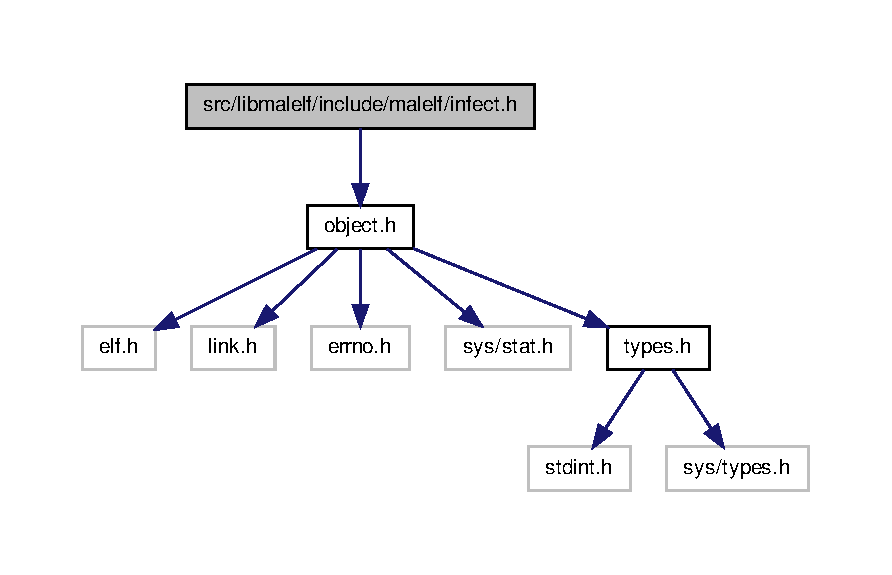
\includegraphics[width=400pt]{infect_8h__incl}
\end{center}
\end{figure}
This graph shows which files directly or indirectly include this file:\nopagebreak
\begin{figure}[H]
\begin{center}
\leavevmode
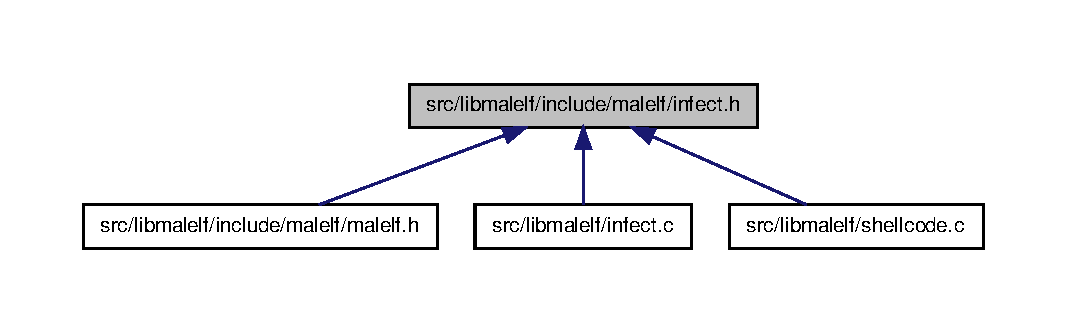
\includegraphics[width=400pt]{infect_8h__dep__incl}
\end{center}
\end{figure}
\subsection*{Defines}
\begin{DoxyCompactItemize}
\item 
\#define \hyperlink{infect_8h_adbd1caeb8d78c4d163b34925888270ec}{MALELF\_\-MAGIC\_\-BYTES}~0x31333337
\end{DoxyCompactItemize}
\subsection*{Functions}
\begin{DoxyCompactItemize}
\item 
\hyperlink{types_8h_af2b0f13cffd24f6dddf794ae0c7472b4}{\_\-u8} \hyperlink{infect_8h_ab2204e6548cea638fdc54fe23b0a2ec0}{malelf\_\-infect\_\-silvio\_\-padding} (\hyperlink{structmalelf__object}{malelf\_\-object} $\ast$input, \hyperlink{structmalelf__object}{malelf\_\-object} $\ast$output, \hyperlink{structmalelf__object}{malelf\_\-object} $\ast$parasite, \hyperlink{types_8h_a07491c35a48354e0e7b56974a04cc3de}{\_\-u32} offset\_\-entry\_\-point, unsigned long int magic\_\-bytes)
\item 
\hyperlink{types_8h_af2b0f13cffd24f6dddf794ae0c7472b4}{\_\-u8} \hyperlink{infect_8h_abc8717a3cc61a5341b72e0c2f898d517}{\_\-malelf\_\-parasite\_\-silvio\_\-padding} (\hyperlink{structmalelf__object}{malelf\_\-object} $\ast$in, \hyperlink{structmalelf__object}{malelf\_\-object} $\ast$out, unsigned int end\_\-of\_\-text, \hyperlink{structmalelf__object}{malelf\_\-object} $\ast$parasite, \hyperlink{types_8h_a07491c35a48354e0e7b56974a04cc3de}{\_\-u32} offset\_\-entry\_\-point, unsigned old\_\-e\_\-entry, unsigned long int magic\_\-bytes)
\end{DoxyCompactItemize}


\subsection{Define Documentation}
\hypertarget{infect_8h_adbd1caeb8d78c4d163b34925888270ec}{
\index{infect.h@{infect.h}!MALELF\_\-MAGIC\_\-BYTES@{MALELF\_\-MAGIC\_\-BYTES}}
\index{MALELF\_\-MAGIC\_\-BYTES@{MALELF\_\-MAGIC\_\-BYTES}!infect.h@{infect.h}}
\subsubsection[{MALELF\_\-MAGIC\_\-BYTES}]{\setlength{\rightskip}{0pt plus 5cm}\#define MALELF\_\-MAGIC\_\-BYTES~0x31333337}}
\label{infect_8h_adbd1caeb8d78c4d163b34925888270ec}


Definition at line 6 of file infect.h.



\subsection{Function Documentation}
\hypertarget{infect_8h_abc8717a3cc61a5341b72e0c2f898d517}{
\index{infect.h@{infect.h}!\_\-malelf\_\-parasite\_\-silvio\_\-padding@{\_\-malelf\_\-parasite\_\-silvio\_\-padding}}
\index{\_\-malelf\_\-parasite\_\-silvio\_\-padding@{\_\-malelf\_\-parasite\_\-silvio\_\-padding}!infect.h@{infect.h}}
\subsubsection[{\_\-malelf\_\-parasite\_\-silvio\_\-padding}]{\setlength{\rightskip}{0pt plus 5cm}{\bf \_\-u8} \_\-malelf\_\-parasite\_\-silvio\_\-padding (
\begin{DoxyParamCaption}
\item[{{\bf malelf\_\-object} $\ast$}]{in, }
\item[{{\bf malelf\_\-object} $\ast$}]{out, }
\item[{unsigned int}]{end\_\-of\_\-text, }
\item[{{\bf malelf\_\-object} $\ast$}]{parasite, }
\item[{{\bf \_\-u32}}]{offset\_\-entry\_\-point, }
\item[{unsigned}]{old\_\-e\_\-entry, }
\item[{unsigned long int}]{magic\_\-bytes}
\end{DoxyParamCaption}
)}}
\label{infect_8h_abc8717a3cc61a5341b72e0c2f898d517}


Definition at line 135 of file infect.c.

\hypertarget{infect_8h_ab2204e6548cea638fdc54fe23b0a2ec0}{
\index{infect.h@{infect.h}!malelf\_\-infect\_\-silvio\_\-padding@{malelf\_\-infect\_\-silvio\_\-padding}}
\index{malelf\_\-infect\_\-silvio\_\-padding@{malelf\_\-infect\_\-silvio\_\-padding}!infect.h@{infect.h}}
\subsubsection[{malelf\_\-infect\_\-silvio\_\-padding}]{\setlength{\rightskip}{0pt plus 5cm}{\bf \_\-u8} malelf\_\-infect\_\-silvio\_\-padding (
\begin{DoxyParamCaption}
\item[{{\bf malelf\_\-object} $\ast$}]{input, }
\item[{{\bf malelf\_\-object} $\ast$}]{output, }
\item[{{\bf malelf\_\-object} $\ast$}]{parasite, }
\item[{{\bf \_\-u32}}]{offset\_\-entry\_\-point, }
\item[{unsigned long int}]{magic\_\-bytes}
\end{DoxyParamCaption}
)}}
\label{infect_8h_ab2204e6548cea638fdc54fe23b0a2ec0}
Try to infect the ELF using the text padding technique created by Silvio Cesare. More information: \href{http://www.win.tue.nl/~aeb/linux/hh/virus/unix-viruses.txt}{\tt http://www.win.tue.nl/$\sim$aeb/linux/hh/virus/unix-\/viruses.txt} 

Definition at line 43 of file infect.c.


\hypertarget{malelf_8h}{
\section{src/libmalelf/include/malelf/malelf.h File Reference}
\label{malelf_8h}\index{src/libmalelf/include/malelf/malelf.h@{src/libmalelf/include/malelf/malelf.h}}
}
{\ttfamily \#include $<$malelf/object.h$>$}\par
{\ttfamily \#include $<$malelf/defines.h$>$}\par
{\ttfamily \#include $<$malelf/error.h$>$}\par
{\ttfamily \#include $<$malelf/util.h$>$}\par
{\ttfamily \#include $<$malelf/disas.h$>$}\par
{\ttfamily \#include $<$malelf/shellcode.h$>$}\par
{\ttfamily \#include $<$malelf/infect.h$>$}\par
{\ttfamily \#include $<$malelf/reverse\_\-elf.h$>$}\par
Include dependency graph for malelf.h:\nopagebreak
\begin{figure}[H]
\begin{center}
\leavevmode
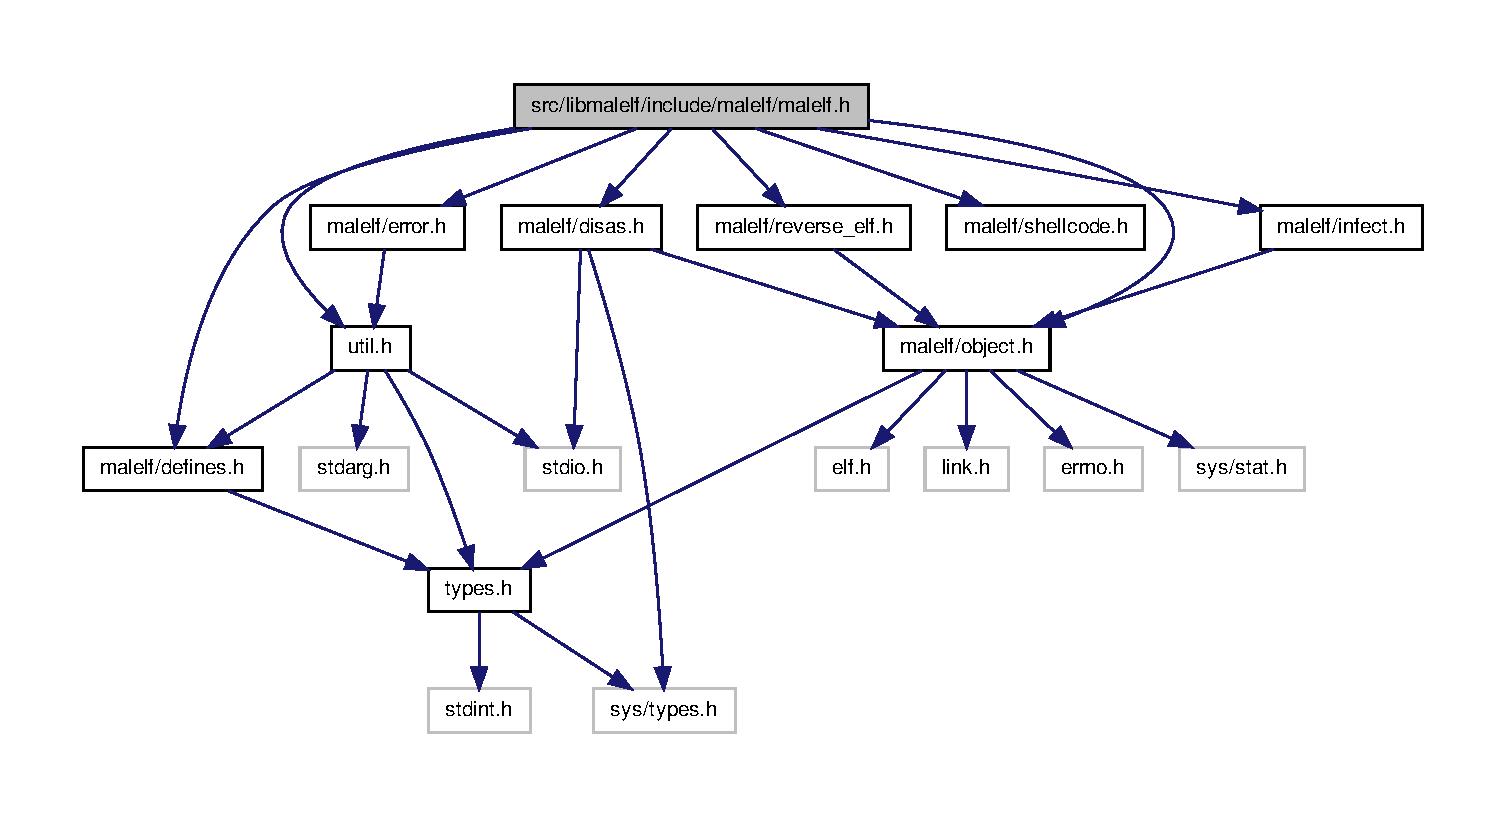
\includegraphics[width=400pt]{malelf_8h__incl}
\end{center}
\end{figure}

\hypertarget{object_8h}{
\section{src/libmalelf/include/malelf/object.h File Reference}
\label{object_8h}\index{src/libmalelf/include/malelf/object.h@{src/libmalelf/include/malelf/object.h}}
}
{\ttfamily \#include $<$elf.h$>$}\par
{\ttfamily \#include $<$link.h$>$}\par
{\ttfamily \#include $<$errno.h$>$}\par
{\ttfamily \#include $<$sys/stat.h$>$}\par
{\ttfamily \#include \char`\"{}types.h\char`\"{}}\par
Include dependency graph for object.h:\nopagebreak
\begin{figure}[H]
\begin{center}
\leavevmode
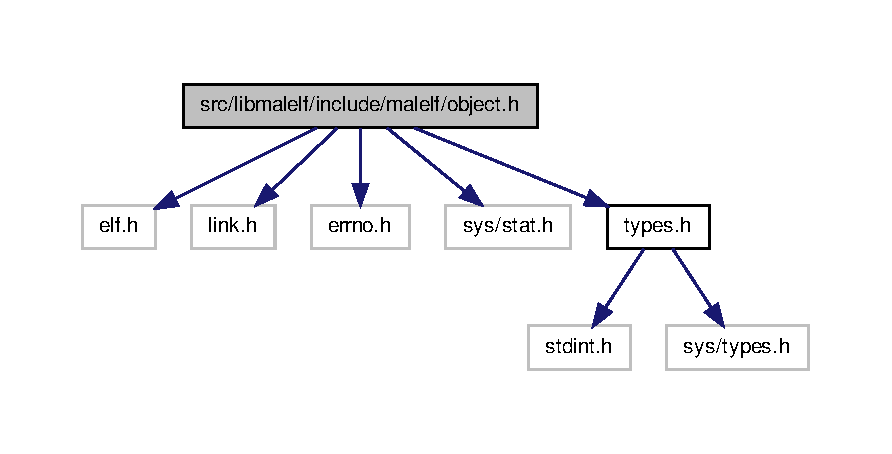
\includegraphics[width=400pt]{object_8h__incl}
\end{center}
\end{figure}
This graph shows which files directly or indirectly include this file:\nopagebreak
\begin{figure}[H]
\begin{center}
\leavevmode
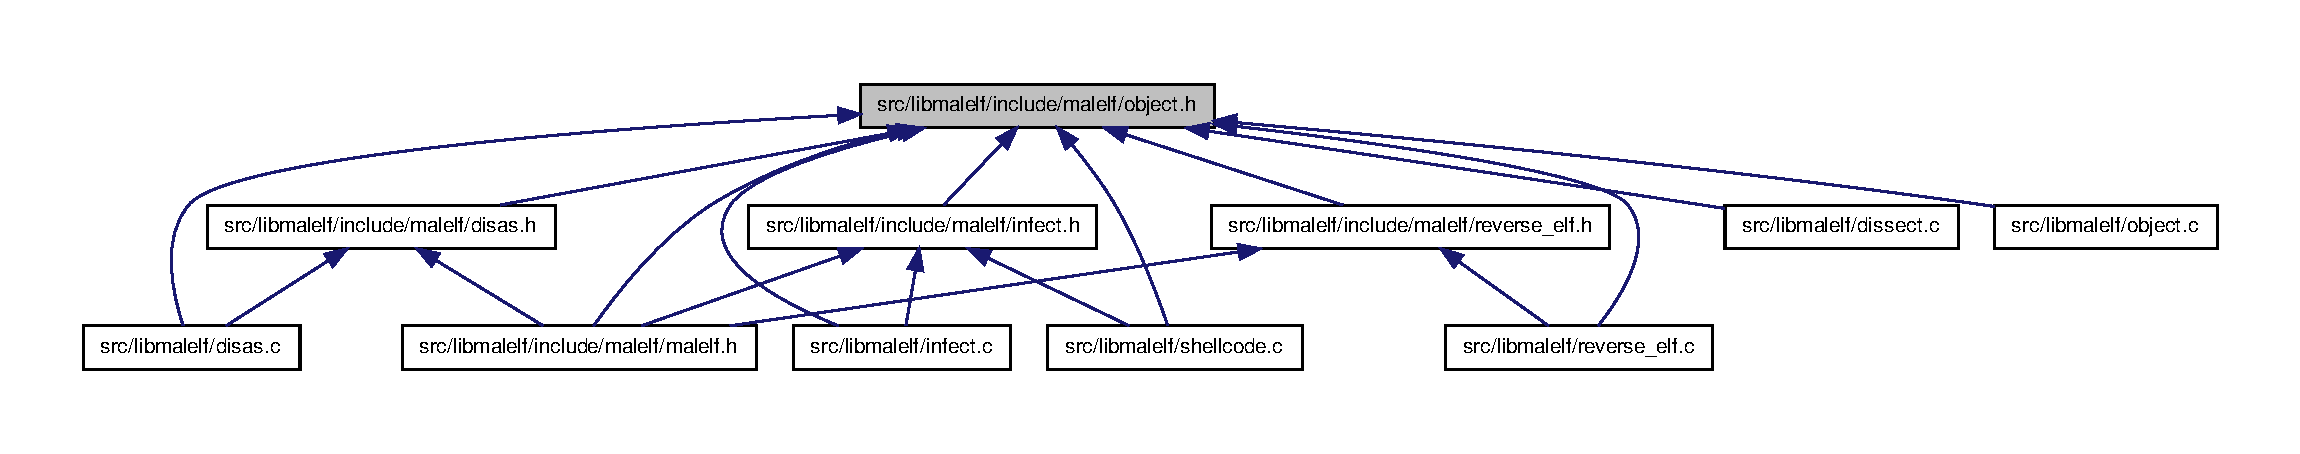
\includegraphics[width=400pt]{object_8h__dep__incl}
\end{center}
\end{figure}
\subsection*{Classes}
\begin{DoxyCompactItemize}
\item 
union \hyperlink{unionmalelf__dword}{malelf\_\-dword}
\item 
struct \hyperlink{structmalelf__elf__t}{malelf\_\-elf\_\-t}
\item 
struct \hyperlink{structmalelf__object}{malelf\_\-object}
\item 
struct \hyperlink{structmalelf__elf__attr}{malelf\_\-elf\_\-attr}
\item 
struct \hyperlink{structmalelf__add__section__t}{malelf\_\-add\_\-section\_\-t}
\end{DoxyCompactItemize}
\subsection*{Defines}
\begin{DoxyCompactItemize}
\item 
\#define \hyperlink{object_8h_a6743b71b8a58ab8376edf49b3cf42636}{GET\_\-ATTR\_\-NAME}(attr)~attr != NULL ? (attr-\/$>$name) : \char`\"{}UNKNOWN\char`\"{}
\item 
\#define \hyperlink{object_8h_a08f951398aa734d26e7ebbedca5c330a}{GET\_\-ATTR\_\-DESC}(attr)~attr != NULL ? (attr-\/$>$desc) : \char`\"{}UNKNOWN\char`\"{}
\item 
\#define \hyperlink{object_8h_a39c18e5458ff5e329030fb2f3b8cf5ac}{GET\_\-SECTION\_\-NAME}(obj, header, sections, sec\_\-idx)~(char$\ast$) (obj-\/$>$mem + sections\mbox{[}header-\/$>$e\_\-shstrndx\mbox{]}.sh\_\-offset + sections\mbox{[}sec\_\-idx\mbox{]}.sh\_\-name)
\item 
\#define \hyperlink{object_8h_af892106ece3d0045a92cf757d9c600ee}{MALELF\_\-MAP\_\-ELF}(obj)
\end{DoxyCompactItemize}
\subsection*{Enumerations}
\begin{DoxyCompactItemize}
\item 
enum \hyperlink{object_8h_a24f8376c4f2e7c8f8c023d1733ab02e9}{alloc\_\-type\_\-t} \{ \hyperlink{object_8h_a24f8376c4f2e7c8f8c023d1733ab02e9ad48c3ed5205532e83d005272cf247088}{ALLOC\_\-MMAP} =  0, 
\hyperlink{object_8h_a24f8376c4f2e7c8f8c023d1733ab02e9a5f6717a7ef93d84ae1ab71597b789971}{ALLOC\_\-MALLOC}
 \}
\end{DoxyCompactItemize}
\subsection*{Functions}
\begin{DoxyCompactItemize}
\item 
void \hyperlink{object_8h_a9036ce6733bf255896811721f303b30f}{malelf\_\-init\_\-object} (\hyperlink{structmalelf__object}{malelf\_\-object} $\ast$)
\begin{DoxyCompactList}\small\item\em Initialize the malelf object data type. \end{DoxyCompactList}\item 
void \hyperlink{object_8h_a4488b6a72bba36d27511d65b454cb158}{read\_\-elf\_\-file} (\hyperlink{structmalelf__object}{malelf\_\-object} $\ast$)
\item 
void \hyperlink{object_8h_a52de7c3bdc0efbd6f87b2286b505f449}{create\_\-elf\_\-file} (\hyperlink{structmalelf__object}{malelf\_\-object} $\ast$)
\item 
\hyperlink{types_8h_af2b0f13cffd24f6dddf794ae0c7472b4}{\_\-u8} \hyperlink{object_8h_a5019afc93abb304c5ccdd1e3f5131d72}{copy\_\-malelf\_\-object\_\-raw} (\hyperlink{structmalelf__object}{malelf\_\-object} $\ast$, \hyperlink{structmalelf__object}{malelf\_\-object} $\ast$)
\item 
\hyperlink{types_8h_aacb1ea6e27efde1c708a8bc4b56ee1a2}{\_\-i32} \hyperlink{object_8h_a54b384361ec6e433175bb58ef217467b}{malelf\_\-open} (\hyperlink{structmalelf__object}{malelf\_\-object} $\ast$obj, char $\ast$filename, int flags)
\begin{DoxyCompactList}\small\item\em Open the binary file 'filename' and fill the struct \hyperlink{structmalelf__object}{malelf\_\-object}. \end{DoxyCompactList}\item 
\hyperlink{types_8h_aacb1ea6e27efde1c708a8bc4b56ee1a2}{\_\-i32} \hyperlink{object_8h_a6daa20f1e4fb72096a9eb27ee0234a85}{malelf\_\-openr} (\hyperlink{structmalelf__object}{malelf\_\-object} $\ast$obj, char $\ast$filename)
\item 
\hyperlink{types_8h_aacb1ea6e27efde1c708a8bc4b56ee1a2}{\_\-i32} \hyperlink{object_8h_a44e74dbe97ac2f3a4571b53cafa3833f}{malelf\_\-openw} (\hyperlink{structmalelf__object}{malelf\_\-object} $\ast$obj, char $\ast$filename)
\item 
\hyperlink{types_8h_a07491c35a48354e0e7b56974a04cc3de}{\_\-u32} \hyperlink{object_8h_a9dc624caa7e16317902d3d5ce93a3b55}{malelf\_\-close} (\hyperlink{structmalelf__object}{malelf\_\-object} $\ast$obj)
\item 
\hyperlink{types_8h_af2b0f13cffd24f6dddf794ae0c7472b4}{\_\-u8} \hyperlink{object_8h_ab72f2409e093e754523c77367c4d92cf}{malelf\_\-check\_\-elf} (\hyperlink{structmalelf__object}{malelf\_\-object} $\ast$obj)
\begin{DoxyCompactList}\small\item\em Check if the binary file mapped in obj is of type ELF. \end{DoxyCompactList}\item 
\hyperlink{types_8h_af2b0f13cffd24f6dddf794ae0c7472b4}{\_\-u8} \hyperlink{object_8h_a705bb64cb648ecd8936c8643bb880b09}{malelf\_\-add\_\-section} (\hyperlink{structmalelf__object}{malelf\_\-object} $\ast$i, \hyperlink{structmalelf__object}{malelf\_\-object} $\ast$o, \hyperlink{structmalelf__add__section__t}{malelf\_\-add\_\-section\_\-t} opt)
\item 
\hyperlink{structmalelf__elf__attr}{malelf\_\-elf\_\-attr} $\ast$ \hyperlink{object_8h_a3ba28c3bb78eea1572e6ee916c73de5e}{get\_\-header\_\-type} (ElfW(Half) etype)
\item 
\hyperlink{structmalelf__elf__attr}{malelf\_\-elf\_\-attr} $\ast$ \hyperlink{object_8h_a2775a595939a915c18d425eb6fd20c82}{get\_\-section\_\-type} (ElfW(Half) stype)
\item 
\hyperlink{structmalelf__elf__attr}{malelf\_\-elf\_\-attr} $\ast$ \hyperlink{object_8h_a5f6d74f6d972ce48a0e59a1f429029b6}{get\_\-machine} (ElfW(Half) emach)
\item 
\hyperlink{structmalelf__elf__attr}{malelf\_\-elf\_\-attr} $\ast$ \hyperlink{object_8h_a99ec39bacadbebc3fdf63963e132e9a6}{get\_\-segment\_\-type} (ElfW(Word) seg)
\item 
void \hyperlink{object_8h_a971197508f3beef099c814f783531895}{pretty\_\-print\_\-elf\_\-header} (ElfW(Ehdr)$\ast$)
\item 
void \hyperlink{object_8h_af8d6c6aa67501fb81bdca9776cb91f9e}{pretty\_\-print\_\-pht} (ElfW(Ehdr)$\ast$, ElfW(Phdr)$\ast$)
\item 
void \hyperlink{object_8h_a6216012206b8aac78cee92d2f9bbd6a6}{pretty\_\-print\_\-sht} (\hyperlink{structmalelf__object}{malelf\_\-object} $\ast$, ElfW(Ehdr)$\ast$, ElfW(Shdr)$\ast$)
\item 
void \hyperlink{object_8h_ae665cd2bb839b13f26324d9ba11d5e0c}{pretty\_\-print\_\-strtab} (\hyperlink{structmalelf__object}{malelf\_\-object} $\ast$, ElfW(Ehdr)$\ast$, ElfW(Shdr)$\ast$)
\end{DoxyCompactItemize}
\subsection*{Variables}
\begin{DoxyCompactItemize}
\item 
\hyperlink{structmalelf__elf__attr}{malelf\_\-elf\_\-attr} \hyperlink{object_8h_acc10cae2b21d17dee26af9734f7868b6}{elf\_\-object\_\-types} \mbox{[}$\,$\mbox{]}
\item 
\hyperlink{structmalelf__elf__attr}{malelf\_\-elf\_\-attr} \hyperlink{object_8h_a3b6e5f8c8d062229d7e9383a2a9fb246}{elf\_\-machine} \mbox{[}$\,$\mbox{]}
\begin{DoxyCompactList}\small\item\em Possible target machines. \end{DoxyCompactList}\item 
\hyperlink{structmalelf__elf__attr}{malelf\_\-elf\_\-attr} \hyperlink{object_8h_a7174cbdd18cf8537c1b49a4c4a56455f}{elf\_\-section\_\-types} \mbox{[}$\,$\mbox{]}
\begin{DoxyCompactList}\small\item\em Possible section types. \end{DoxyCompactList}\item 
\hyperlink{structmalelf__elf__attr}{malelf\_\-elf\_\-attr} \hyperlink{object_8h_ac3502bce5138fd64604041f1955901c0}{elf\_\-segment\_\-types} \mbox{[}$\,$\mbox{]}
\begin{DoxyCompactList}\small\item\em Possible segment types. \end{DoxyCompactList}\item 
\hyperlink{structmalelf__elf__attr}{malelf\_\-elf\_\-attr} \hyperlink{object_8h_a32503e0e5e17c5c84a14ff7940ad78c9}{elf\_\-segment\_\-flags} \mbox{[}$\,$\mbox{]}
\begin{DoxyCompactList}\small\item\em Possible segment flags. \end{DoxyCompactList}\end{DoxyCompactItemize}


\subsection{Define Documentation}
\hypertarget{object_8h_a08f951398aa734d26e7ebbedca5c330a}{
\index{object.h@{object.h}!GET\_\-ATTR\_\-DESC@{GET\_\-ATTR\_\-DESC}}
\index{GET\_\-ATTR\_\-DESC@{GET\_\-ATTR\_\-DESC}!object.h@{object.h}}
\subsubsection[{GET\_\-ATTR\_\-DESC}]{\setlength{\rightskip}{0pt plus 5cm}\#define GET\_\-ATTR\_\-DESC(
\begin{DoxyParamCaption}
\item[{}]{attr}
\end{DoxyParamCaption}
)~attr != NULL ? (attr-\/$>$desc) : \char`\"{}UNKNOWN\char`\"{}}}
\label{object_8h_a08f951398aa734d26e7ebbedca5c330a}


Definition at line 11 of file object.h.

\hypertarget{object_8h_a6743b71b8a58ab8376edf49b3cf42636}{
\index{object.h@{object.h}!GET\_\-ATTR\_\-NAME@{GET\_\-ATTR\_\-NAME}}
\index{GET\_\-ATTR\_\-NAME@{GET\_\-ATTR\_\-NAME}!object.h@{object.h}}
\subsubsection[{GET\_\-ATTR\_\-NAME}]{\setlength{\rightskip}{0pt plus 5cm}\#define GET\_\-ATTR\_\-NAME(
\begin{DoxyParamCaption}
\item[{}]{attr}
\end{DoxyParamCaption}
)~attr != NULL ? (attr-\/$>$name) : \char`\"{}UNKNOWN\char`\"{}}}
\label{object_8h_a6743b71b8a58ab8376edf49b3cf42636}


Definition at line 10 of file object.h.

\hypertarget{object_8h_a39c18e5458ff5e329030fb2f3b8cf5ac}{
\index{object.h@{object.h}!GET\_\-SECTION\_\-NAME@{GET\_\-SECTION\_\-NAME}}
\index{GET\_\-SECTION\_\-NAME@{GET\_\-SECTION\_\-NAME}!object.h@{object.h}}
\subsubsection[{GET\_\-SECTION\_\-NAME}]{\setlength{\rightskip}{0pt plus 5cm}\#define GET\_\-SECTION\_\-NAME(
\begin{DoxyParamCaption}
\item[{}]{obj, }
\item[{}]{header, }
\item[{}]{sections, }
\item[{}]{sec\_\-idx}
\end{DoxyParamCaption}
)~(char$\ast$) (obj-\/$>$mem + sections\mbox{[}header-\/$>$e\_\-shstrndx\mbox{]}.sh\_\-offset + sections\mbox{[}sec\_\-idx\mbox{]}.sh\_\-name)}}
\label{object_8h_a39c18e5458ff5e329030fb2f3b8cf5ac}


Definition at line 13 of file object.h.

\hypertarget{object_8h_af892106ece3d0045a92cf757d9c600ee}{
\index{object.h@{object.h}!MALELF\_\-MAP\_\-ELF@{MALELF\_\-MAP\_\-ELF}}
\index{MALELF\_\-MAP\_\-ELF@{MALELF\_\-MAP\_\-ELF}!object.h@{object.h}}
\subsubsection[{MALELF\_\-MAP\_\-ELF}]{\setlength{\rightskip}{0pt plus 5cm}\#define MALELF\_\-MAP\_\-ELF(
\begin{DoxyParamCaption}
\item[{}]{obj}
\end{DoxyParamCaption}
)}}
\label{object_8h_af892106ece3d0045a92cf757d9c600ee}
{\bfseries Value:}
\begin{DoxyCode}
do {\
  assert(obj->mem != NULL);\
  obj->elf.elfh = (ElfW(Ehdr)*) obj->mem;\
  assert(obj->elf.elfh != NULL); \
  assert((off_t)obj->elf.elfh->e_phoff < obj->st_info.st_size); \
  assert((off_t)obj->elf.elfh->e_shoff < obj->st_info.st_size);         \
  obj->elf.elfp = (ElfW(Phdr)*) (obj->mem + obj->elf.elfh->e_phoff);\
  obj->elf.elfs = (ElfW(Shdr)*) (obj->mem + obj->elf.elfh->e_shoff);\
  } while(0)
\end{DoxyCode}


Definition at line 14 of file object.h.



\subsection{Enumeration Type Documentation}
\hypertarget{object_8h_a24f8376c4f2e7c8f8c023d1733ab02e9}{
\index{object.h@{object.h}!alloc\_\-type\_\-t@{alloc\_\-type\_\-t}}
\index{alloc\_\-type\_\-t@{alloc\_\-type\_\-t}!object.h@{object.h}}
\subsubsection[{alloc\_\-type\_\-t}]{\setlength{\rightskip}{0pt plus 5cm}enum {\bf alloc\_\-type\_\-t}}}
\label{object_8h_a24f8376c4f2e7c8f8c023d1733ab02e9}
\begin{Desc}
\item[Enumerator: ]\par
\begin{description}
\index{ALLOC\_\-MMAP@{ALLOC\_\-MMAP}!object.h@{object.h}}\index{object.h@{object.h}!ALLOC\_\-MMAP@{ALLOC\_\-MMAP}}\item[{\em 
\hypertarget{object_8h_a24f8376c4f2e7c8f8c023d1733ab02e9ad48c3ed5205532e83d005272cf247088}{
ALLOC\_\-MMAP}
\label{object_8h_a24f8376c4f2e7c8f8c023d1733ab02e9ad48c3ed5205532e83d005272cf247088}
}]\index{ALLOC\_\-MALLOC@{ALLOC\_\-MALLOC}!object.h@{object.h}}\index{object.h@{object.h}!ALLOC\_\-MALLOC@{ALLOC\_\-MALLOC}}\item[{\em 
\hypertarget{object_8h_a24f8376c4f2e7c8f8c023d1733ab02e9a5f6717a7ef93d84ae1ab71597b789971}{
ALLOC\_\-MALLOC}
\label{object_8h_a24f8376c4f2e7c8f8c023d1733ab02e9a5f6717a7ef93d84ae1ab71597b789971}
}]\end{description}
\end{Desc}



Definition at line 24 of file object.h.



\subsection{Function Documentation}
\hypertarget{object_8h_a5019afc93abb304c5ccdd1e3f5131d72}{
\index{object.h@{object.h}!copy\_\-malelf\_\-object\_\-raw@{copy\_\-malelf\_\-object\_\-raw}}
\index{copy\_\-malelf\_\-object\_\-raw@{copy\_\-malelf\_\-object\_\-raw}!object.h@{object.h}}
\subsubsection[{copy\_\-malelf\_\-object\_\-raw}]{\setlength{\rightskip}{0pt plus 5cm}{\bf \_\-u8} copy\_\-malelf\_\-object\_\-raw (
\begin{DoxyParamCaption}
\item[{{\bf malelf\_\-object} $\ast$}]{, }
\item[{{\bf malelf\_\-object} $\ast$}]{}
\end{DoxyParamCaption}
)}}
\label{object_8h_a5019afc93abb304c5ccdd1e3f5131d72}


Definition at line 302 of file object.c.

\hypertarget{object_8h_a52de7c3bdc0efbd6f87b2286b505f449}{
\index{object.h@{object.h}!create\_\-elf\_\-file@{create\_\-elf\_\-file}}
\index{create\_\-elf\_\-file@{create\_\-elf\_\-file}!object.h@{object.h}}
\subsubsection[{create\_\-elf\_\-file}]{\setlength{\rightskip}{0pt plus 5cm}void create\_\-elf\_\-file (
\begin{DoxyParamCaption}
\item[{{\bf malelf\_\-object} $\ast$}]{}
\end{DoxyParamCaption}
)}}
\label{object_8h_a52de7c3bdc0efbd6f87b2286b505f449}
\hypertarget{object_8h_a3ba28c3bb78eea1572e6ee916c73de5e}{
\index{object.h@{object.h}!get\_\-header\_\-type@{get\_\-header\_\-type}}
\index{get\_\-header\_\-type@{get\_\-header\_\-type}!object.h@{object.h}}
\subsubsection[{get\_\-header\_\-type}]{\setlength{\rightskip}{0pt plus 5cm}{\bf malelf\_\-elf\_\-attr}$\ast$ get\_\-header\_\-type (
\begin{DoxyParamCaption}
\item[{ElfW(Half)}]{etype}
\end{DoxyParamCaption}
)}}
\label{object_8h_a3ba28c3bb78eea1572e6ee916c73de5e}


Definition at line 254 of file object.c.

\hypertarget{object_8h_a5f6d74f6d972ce48a0e59a1f429029b6}{
\index{object.h@{object.h}!get\_\-machine@{get\_\-machine}}
\index{get\_\-machine@{get\_\-machine}!object.h@{object.h}}
\subsubsection[{get\_\-machine}]{\setlength{\rightskip}{0pt plus 5cm}{\bf malelf\_\-elf\_\-attr}$\ast$ get\_\-machine (
\begin{DoxyParamCaption}
\item[{ElfW(Half)}]{emach}
\end{DoxyParamCaption}
)}}
\label{object_8h_a5f6d74f6d972ce48a0e59a1f429029b6}


Definition at line 278 of file object.c.

\hypertarget{object_8h_a2775a595939a915c18d425eb6fd20c82}{
\index{object.h@{object.h}!get\_\-section\_\-type@{get\_\-section\_\-type}}
\index{get\_\-section\_\-type@{get\_\-section\_\-type}!object.h@{object.h}}
\subsubsection[{get\_\-section\_\-type}]{\setlength{\rightskip}{0pt plus 5cm}{\bf malelf\_\-elf\_\-attr}$\ast$ get\_\-section\_\-type (
\begin{DoxyParamCaption}
\item[{ElfW(Half)}]{stype}
\end{DoxyParamCaption}
)}}
\label{object_8h_a2775a595939a915c18d425eb6fd20c82}


Definition at line 266 of file object.c.

\hypertarget{object_8h_a99ec39bacadbebc3fdf63963e132e9a6}{
\index{object.h@{object.h}!get\_\-segment\_\-type@{get\_\-segment\_\-type}}
\index{get\_\-segment\_\-type@{get\_\-segment\_\-type}!object.h@{object.h}}
\subsubsection[{get\_\-segment\_\-type}]{\setlength{\rightskip}{0pt plus 5cm}{\bf malelf\_\-elf\_\-attr}$\ast$ get\_\-segment\_\-type (
\begin{DoxyParamCaption}
\item[{ElfW(Word)}]{seg}
\end{DoxyParamCaption}
)}}
\label{object_8h_a99ec39bacadbebc3fdf63963e132e9a6}


Definition at line 290 of file object.c.

\hypertarget{object_8h_a705bb64cb648ecd8936c8643bb880b09}{
\index{object.h@{object.h}!malelf\_\-add\_\-section@{malelf\_\-add\_\-section}}
\index{malelf\_\-add\_\-section@{malelf\_\-add\_\-section}!object.h@{object.h}}
\subsubsection[{malelf\_\-add\_\-section}]{\setlength{\rightskip}{0pt plus 5cm}{\bf \_\-u8} malelf\_\-add\_\-section (
\begin{DoxyParamCaption}
\item[{{\bf malelf\_\-object} $\ast$}]{i, }
\item[{{\bf malelf\_\-object} $\ast$}]{o, }
\item[{{\bf malelf\_\-add\_\-section\_\-t}}]{opt}
\end{DoxyParamCaption}
)}}
\label{object_8h_a705bb64cb648ecd8936c8643bb880b09}


Definition at line 209 of file object.c.

\hypertarget{object_8h_ab72f2409e093e754523c77367c4d92cf}{
\index{object.h@{object.h}!malelf\_\-check\_\-elf@{malelf\_\-check\_\-elf}}
\index{malelf\_\-check\_\-elf@{malelf\_\-check\_\-elf}!object.h@{object.h}}
\subsubsection[{malelf\_\-check\_\-elf}]{\setlength{\rightskip}{0pt plus 5cm}{\bf \_\-u8} malelf\_\-check\_\-elf (
\begin{DoxyParamCaption}
\item[{{\bf malelf\_\-object} $\ast$}]{obj}
\end{DoxyParamCaption}
)}}
\label{object_8h_ab72f2409e093e754523c77367c4d92cf}


Check if the binary file mapped in obj is of type ELF. 


\begin{DoxyParams}{Parameters}
{\em malelf\_\-object$\ast$} & Malelf object type \\
\hline
\end{DoxyParams}
\begin{DoxyReturn}{Returns}
\_\-u8 Returns a malelf\_\-status enum number. 
\end{DoxyReturn}


Definition at line 117 of file object.c.

\hypertarget{object_8h_a9dc624caa7e16317902d3d5ce93a3b55}{
\index{object.h@{object.h}!malelf\_\-close@{malelf\_\-close}}
\index{malelf\_\-close@{malelf\_\-close}!object.h@{object.h}}
\subsubsection[{malelf\_\-close}]{\setlength{\rightskip}{0pt plus 5cm}{\bf \_\-u32} malelf\_\-close (
\begin{DoxyParamCaption}
\item[{{\bf malelf\_\-object} $\ast$}]{obj}
\end{DoxyParamCaption}
)}}
\label{object_8h_a9dc624caa7e16317902d3d5ce93a3b55}


Definition at line 195 of file object.c.

\hypertarget{object_8h_a9036ce6733bf255896811721f303b30f}{
\index{object.h@{object.h}!malelf\_\-init\_\-object@{malelf\_\-init\_\-object}}
\index{malelf\_\-init\_\-object@{malelf\_\-init\_\-object}!object.h@{object.h}}
\subsubsection[{malelf\_\-init\_\-object}]{\setlength{\rightskip}{0pt plus 5cm}void malelf\_\-init\_\-object (
\begin{DoxyParamCaption}
\item[{{\bf malelf\_\-object} $\ast$}]{obj}
\end{DoxyParamCaption}
)}}
\label{object_8h_a9036ce6733bf255896811721f303b30f}


Initialize the malelf object data type. 

Never forget to call this function before use the malelf API with \hyperlink{structmalelf__object}{malelf\_\-object}.


\begin{DoxyParams}{Parameters}
{\em malelf\_\-object$\ast$} & Malelf object type \\
\hline
\end{DoxyParams}
\begin{DoxyReturn}{Returns}
void 
\end{DoxyReturn}


Definition at line 102 of file object.c.

\hypertarget{object_8h_a54b384361ec6e433175bb58ef217467b}{
\index{object.h@{object.h}!malelf\_\-open@{malelf\_\-open}}
\index{malelf\_\-open@{malelf\_\-open}!object.h@{object.h}}
\subsubsection[{malelf\_\-open}]{\setlength{\rightskip}{0pt plus 5cm}{\bf \_\-i32} malelf\_\-open (
\begin{DoxyParamCaption}
\item[{{\bf malelf\_\-object} $\ast$}]{obj, }
\item[{char $\ast$}]{filename, }
\item[{int}]{flags}
\end{DoxyParamCaption}
)}}
\label{object_8h_a54b384361ec6e433175bb58ef217467b}


Open the binary file 'filename' and fill the struct \hyperlink{structmalelf__object}{malelf\_\-object}. 

Uses mmap to map the binary in memory.


\begin{DoxyParams}{Parameters}
{\em malelf\_\-object$\ast$} & obj \\
\hline
{\em char$\ast$} & filename \\
\hline
{\em int} & flags \\
\hline
\end{DoxyParams}


If the file was created right now, then there is no buffer to map in memory.



Definition at line 144 of file object.c.

\hypertarget{object_8h_a6daa20f1e4fb72096a9eb27ee0234a85}{
\index{object.h@{object.h}!malelf\_\-openr@{malelf\_\-openr}}
\index{malelf\_\-openr@{malelf\_\-openr}!object.h@{object.h}}
\subsubsection[{malelf\_\-openr}]{\setlength{\rightskip}{0pt plus 5cm}{\bf \_\-i32} malelf\_\-openr (
\begin{DoxyParamCaption}
\item[{{\bf malelf\_\-object} $\ast$}]{obj, }
\item[{char $\ast$}]{filename}
\end{DoxyParamCaption}
)}}
\label{object_8h_a6daa20f1e4fb72096a9eb27ee0234a85}


Definition at line 185 of file object.c.

\hypertarget{object_8h_a44e74dbe97ac2f3a4571b53cafa3833f}{
\index{object.h@{object.h}!malelf\_\-openw@{malelf\_\-openw}}
\index{malelf\_\-openw@{malelf\_\-openw}!object.h@{object.h}}
\subsubsection[{malelf\_\-openw}]{\setlength{\rightskip}{0pt plus 5cm}{\bf \_\-i32} malelf\_\-openw (
\begin{DoxyParamCaption}
\item[{{\bf malelf\_\-object} $\ast$}]{obj, }
\item[{char $\ast$}]{filename}
\end{DoxyParamCaption}
)}}
\label{object_8h_a44e74dbe97ac2f3a4571b53cafa3833f}


Definition at line 190 of file object.c.

\hypertarget{object_8h_a971197508f3beef099c814f783531895}{
\index{object.h@{object.h}!pretty\_\-print\_\-elf\_\-header@{pretty\_\-print\_\-elf\_\-header}}
\index{pretty\_\-print\_\-elf\_\-header@{pretty\_\-print\_\-elf\_\-header}!object.h@{object.h}}
\subsubsection[{pretty\_\-print\_\-elf\_\-header}]{\setlength{\rightskip}{0pt plus 5cm}void pretty\_\-print\_\-elf\_\-header (
\begin{DoxyParamCaption}
\item[{ElfW(Ehdr)$\ast$}]{}
\end{DoxyParamCaption}
)}}
\label{object_8h_a971197508f3beef099c814f783531895}


Definition at line 63 of file dissect.c.

\hypertarget{object_8h_af8d6c6aa67501fb81bdca9776cb91f9e}{
\index{object.h@{object.h}!pretty\_\-print\_\-pht@{pretty\_\-print\_\-pht}}
\index{pretty\_\-print\_\-pht@{pretty\_\-print\_\-pht}!object.h@{object.h}}
\subsubsection[{pretty\_\-print\_\-pht}]{\setlength{\rightskip}{0pt plus 5cm}void pretty\_\-print\_\-pht (
\begin{DoxyParamCaption}
\item[{ElfW(Ehdr)$\ast$}]{, }
\item[{ElfW(Phdr)$\ast$}]{}
\end{DoxyParamCaption}
)}}
\label{object_8h_af8d6c6aa67501fb81bdca9776cb91f9e}


Definition at line 157 of file dissect.c.

\hypertarget{object_8h_a6216012206b8aac78cee92d2f9bbd6a6}{
\index{object.h@{object.h}!pretty\_\-print\_\-sht@{pretty\_\-print\_\-sht}}
\index{pretty\_\-print\_\-sht@{pretty\_\-print\_\-sht}!object.h@{object.h}}
\subsubsection[{pretty\_\-print\_\-sht}]{\setlength{\rightskip}{0pt plus 5cm}void pretty\_\-print\_\-sht (
\begin{DoxyParamCaption}
\item[{{\bf malelf\_\-object} $\ast$}]{, }
\item[{ElfW(Ehdr)$\ast$}]{, }
\item[{ElfW(Shdr)$\ast$}]{}
\end{DoxyParamCaption}
)}}
\label{object_8h_a6216012206b8aac78cee92d2f9bbd6a6}


Definition at line 196 of file dissect.c.

\hypertarget{object_8h_ae665cd2bb839b13f26324d9ba11d5e0c}{
\index{object.h@{object.h}!pretty\_\-print\_\-strtab@{pretty\_\-print\_\-strtab}}
\index{pretty\_\-print\_\-strtab@{pretty\_\-print\_\-strtab}!object.h@{object.h}}
\subsubsection[{pretty\_\-print\_\-strtab}]{\setlength{\rightskip}{0pt plus 5cm}void pretty\_\-print\_\-strtab (
\begin{DoxyParamCaption}
\item[{{\bf malelf\_\-object} $\ast$}]{elf, }
\item[{ElfW(Ehdr)$\ast$}]{header, }
\item[{ElfW(Shdr)$\ast$}]{sections}
\end{DoxyParamCaption}
)}}
\label{object_8h_ae665cd2bb839b13f26324d9ba11d5e0c}
Algorithm based on Elfrw function elfr\_\-symtable\_\-dump at (\href{https://github.com/felipensp/ELFrw}{\tt https://github.com/felipensp/ELFrw})

TODO: $\ast$rewrite this$\ast$ 

Definition at line 257 of file dissect.c.

\hypertarget{object_8h_a4488b6a72bba36d27511d65b454cb158}{
\index{object.h@{object.h}!read\_\-elf\_\-file@{read\_\-elf\_\-file}}
\index{read\_\-elf\_\-file@{read\_\-elf\_\-file}!object.h@{object.h}}
\subsubsection[{read\_\-elf\_\-file}]{\setlength{\rightskip}{0pt plus 5cm}void read\_\-elf\_\-file (
\begin{DoxyParamCaption}
\item[{{\bf malelf\_\-object} $\ast$}]{}
\end{DoxyParamCaption}
)}}
\label{object_8h_a4488b6a72bba36d27511d65b454cb158}


\subsection{Variable Documentation}
\hypertarget{object_8h_a3b6e5f8c8d062229d7e9383a2a9fb246}{
\index{object.h@{object.h}!elf\_\-machine@{elf\_\-machine}}
\index{elf\_\-machine@{elf\_\-machine}!object.h@{object.h}}
\subsubsection[{elf\_\-machine}]{\setlength{\rightskip}{0pt plus 5cm}{\bf malelf\_\-elf\_\-attr} {\bf elf\_\-machine}\mbox{[}$\,$\mbox{]}}}
\label{object_8h_a3b6e5f8c8d062229d7e9383a2a9fb246}


Possible target machines. 



Definition at line 68 of file object.c.

\hypertarget{object_8h_acc10cae2b21d17dee26af9734f7868b6}{
\index{object.h@{object.h}!elf\_\-object\_\-types@{elf\_\-object\_\-types}}
\index{elf\_\-object\_\-types@{elf\_\-object\_\-types}!object.h@{object.h}}
\subsubsection[{elf\_\-object\_\-types}]{\setlength{\rightskip}{0pt plus 5cm}{\bf malelf\_\-elf\_\-attr} {\bf elf\_\-object\_\-types}\mbox{[}$\,$\mbox{]}}}
\label{object_8h_acc10cae2b21d17dee26af9734f7868b6}
\hypertarget{object_8h_a7174cbdd18cf8537c1b49a4c4a56455f}{
\index{object.h@{object.h}!elf\_\-section\_\-types@{elf\_\-section\_\-types}}
\index{elf\_\-section\_\-types@{elf\_\-section\_\-types}!object.h@{object.h}}
\subsubsection[{elf\_\-section\_\-types}]{\setlength{\rightskip}{0pt plus 5cm}{\bf malelf\_\-elf\_\-attr} {\bf elf\_\-section\_\-types}\mbox{[}$\,$\mbox{]}}}
\label{object_8h_a7174cbdd18cf8537c1b49a4c4a56455f}


Possible section types. 



Definition at line 75 of file object.c.

\hypertarget{object_8h_a32503e0e5e17c5c84a14ff7940ad78c9}{
\index{object.h@{object.h}!elf\_\-segment\_\-flags@{elf\_\-segment\_\-flags}}
\index{elf\_\-segment\_\-flags@{elf\_\-segment\_\-flags}!object.h@{object.h}}
\subsubsection[{elf\_\-segment\_\-flags}]{\setlength{\rightskip}{0pt plus 5cm}{\bf malelf\_\-elf\_\-attr} {\bf elf\_\-segment\_\-flags}\mbox{[}$\,$\mbox{]}}}
\label{object_8h_a32503e0e5e17c5c84a14ff7940ad78c9}


Possible segment flags. 



Definition at line 89 of file object.c.

\hypertarget{object_8h_ac3502bce5138fd64604041f1955901c0}{
\index{object.h@{object.h}!elf\_\-segment\_\-types@{elf\_\-segment\_\-types}}
\index{elf\_\-segment\_\-types@{elf\_\-segment\_\-types}!object.h@{object.h}}
\subsubsection[{elf\_\-segment\_\-types}]{\setlength{\rightskip}{0pt plus 5cm}{\bf malelf\_\-elf\_\-attr} {\bf elf\_\-segment\_\-types}\mbox{[}$\,$\mbox{]}}}
\label{object_8h_ac3502bce5138fd64604041f1955901c0}


Possible segment types. 



Definition at line 82 of file object.c.


\hypertarget{print__table_8h}{
\section{src/libmalelf/include/malelf/print\_\-table.h File Reference}
\label{print__table_8h}\index{src/libmalelf/include/malelf/print\_\-table.h@{src/libmalelf/include/malelf/print\_\-table.h}}
}
This graph shows which files directly or indirectly include this file:\nopagebreak
\begin{figure}[H]
\begin{center}
\leavevmode
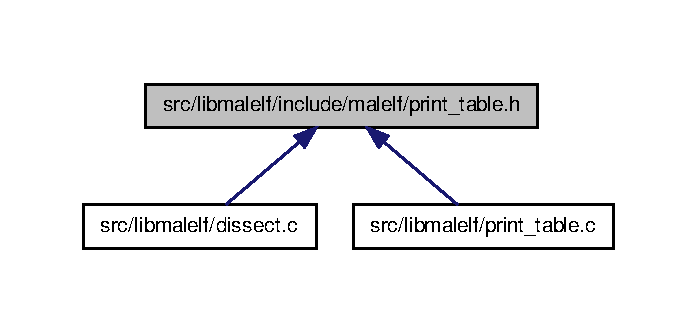
\includegraphics[width=334pt]{print__table_8h__dep__incl}
\end{center}
\end{figure}
\subsection*{Classes}
\begin{DoxyCompactItemize}
\item 
struct \hyperlink{structtb__column}{tb\_\-column}
\item 
struct \hyperlink{structtb__line}{tb\_\-line}
\end{DoxyCompactItemize}
\subsection*{Defines}
\begin{DoxyCompactItemize}
\item 
\#define \hyperlink{print__table_8h_a549e26b0208bdad59ec0d83d711dc018}{SET\_\-COLNAME}(col, str)~strncpy(col.name, str, 80); (col.size = 0)
\end{DoxyCompactItemize}
\subsection*{Typedefs}
\begin{DoxyCompactItemize}
\item 
typedef \hyperlink{structtb__line}{tb\_\-line} \hyperlink{print__table_8h_a0b1577938e3b6fd39373ffc431157ad5}{tb\_\-header}
\item 
typedef \hyperlink{structtb__line}{tb\_\-line} \hyperlink{print__table_8h_a9957462c6e60c222284c883663df3c47}{tb\_\-generic\_\-line}
\end{DoxyCompactItemize}
\subsection*{Functions}
\begin{DoxyCompactItemize}
\item 
void \hyperlink{print__table_8h_a91d724e17c03d2e4e3f5a0cecd4a496a}{print\_\-table\_\-generic} (\hyperlink{structtb__line}{tb\_\-line} $\ast$, int, int, int)
\item 
void \hyperlink{print__table_8h_ad666266f8e36f9f7718af128f545d7a8}{print\_\-table\_\-line} (\hyperlink{structtb__line}{tb\_\-line} $\ast$, int, int)
\item 
void \hyperlink{print__table_8h_a0eb2aa8e2bd01a36f18b8874f07c6be3}{print\_\-table\_\-header} (\hyperlink{structtb__line}{tb\_\-header} $\ast$, int, int)
\item 
void \hyperlink{print__table_8h_aec6ee2c7cfaccd010e6e6f433fd5938e}{print\_\-table\_\-header\_\-art} (int, int)
\end{DoxyCompactItemize}


\subsection{Define Documentation}
\hypertarget{print__table_8h_a549e26b0208bdad59ec0d83d711dc018}{
\index{print\_\-table.h@{print\_\-table.h}!SET\_\-COLNAME@{SET\_\-COLNAME}}
\index{SET\_\-COLNAME@{SET\_\-COLNAME}!print_table.h@{print\_\-table.h}}
\subsubsection[{SET\_\-COLNAME}]{\setlength{\rightskip}{0pt plus 5cm}\#define SET\_\-COLNAME(
\begin{DoxyParamCaption}
\item[{}]{col, }
\item[{}]{str}
\end{DoxyParamCaption}
)~strncpy(col.name, str, 80); (col.size = 0)}}
\label{print__table_8h_a549e26b0208bdad59ec0d83d711dc018}


Definition at line 17 of file print\_\-table.h.



\subsection{Typedef Documentation}
\hypertarget{print__table_8h_a9957462c6e60c222284c883663df3c47}{
\index{print\_\-table.h@{print\_\-table.h}!tb\_\-generic\_\-line@{tb\_\-generic\_\-line}}
\index{tb\_\-generic\_\-line@{tb\_\-generic\_\-line}!print_table.h@{print\_\-table.h}}
\subsubsection[{tb\_\-generic\_\-line}]{\setlength{\rightskip}{0pt plus 5cm}typedef {\bf tb\_\-line} {\bf tb\_\-generic\_\-line}}}
\label{print__table_8h_a9957462c6e60c222284c883663df3c47}


Definition at line 15 of file print\_\-table.h.

\hypertarget{print__table_8h_a0b1577938e3b6fd39373ffc431157ad5}{
\index{print\_\-table.h@{print\_\-table.h}!tb\_\-header@{tb\_\-header}}
\index{tb\_\-header@{tb\_\-header}!print_table.h@{print\_\-table.h}}
\subsubsection[{tb\_\-header}]{\setlength{\rightskip}{0pt plus 5cm}typedef {\bf tb\_\-line} {\bf tb\_\-header}}}
\label{print__table_8h_a0b1577938e3b6fd39373ffc431157ad5}


Definition at line 14 of file print\_\-table.h.



\subsection{Function Documentation}
\hypertarget{print__table_8h_a91d724e17c03d2e4e3f5a0cecd4a496a}{
\index{print\_\-table.h@{print\_\-table.h}!print\_\-table\_\-generic@{print\_\-table\_\-generic}}
\index{print\_\-table\_\-generic@{print\_\-table\_\-generic}!print_table.h@{print\_\-table.h}}
\subsubsection[{print\_\-table\_\-generic}]{\setlength{\rightskip}{0pt plus 5cm}void print\_\-table\_\-generic (
\begin{DoxyParamCaption}
\item[{{\bf tb\_\-line} $\ast$}]{, }
\item[{int}]{, }
\item[{int}]{, }
\item[{int}]{}
\end{DoxyParamCaption}
)}}
\label{print__table_8h_a91d724e17c03d2e4e3f5a0cecd4a496a}
\hypertarget{print__table_8h_a0eb2aa8e2bd01a36f18b8874f07c6be3}{
\index{print\_\-table.h@{print\_\-table.h}!print\_\-table\_\-header@{print\_\-table\_\-header}}
\index{print\_\-table\_\-header@{print\_\-table\_\-header}!print_table.h@{print\_\-table.h}}
\subsubsection[{print\_\-table\_\-header}]{\setlength{\rightskip}{0pt plus 5cm}void print\_\-table\_\-header (
\begin{DoxyParamCaption}
\item[{{\bf tb\_\-header} $\ast$}]{, }
\item[{int}]{, }
\item[{int}]{}
\end{DoxyParamCaption}
)}}
\label{print__table_8h_a0eb2aa8e2bd01a36f18b8874f07c6be3}


Definition at line 137 of file print\_\-table.c.

\hypertarget{print__table_8h_aec6ee2c7cfaccd010e6e6f433fd5938e}{
\index{print\_\-table.h@{print\_\-table.h}!print\_\-table\_\-header\_\-art@{print\_\-table\_\-header\_\-art}}
\index{print\_\-table\_\-header\_\-art@{print\_\-table\_\-header\_\-art}!print_table.h@{print\_\-table.h}}
\subsubsection[{print\_\-table\_\-header\_\-art}]{\setlength{\rightskip}{0pt plus 5cm}void print\_\-table\_\-header\_\-art (
\begin{DoxyParamCaption}
\item[{int}]{, }
\item[{int}]{}
\end{DoxyParamCaption}
)}}
\label{print__table_8h_aec6ee2c7cfaccd010e6e6f433fd5938e}


Definition at line 145 of file print\_\-table.c.

\hypertarget{print__table_8h_ad666266f8e36f9f7718af128f545d7a8}{
\index{print\_\-table.h@{print\_\-table.h}!print\_\-table\_\-line@{print\_\-table\_\-line}}
\index{print\_\-table\_\-line@{print\_\-table\_\-line}!print_table.h@{print\_\-table.h}}
\subsubsection[{print\_\-table\_\-line}]{\setlength{\rightskip}{0pt plus 5cm}void print\_\-table\_\-line (
\begin{DoxyParamCaption}
\item[{{\bf tb\_\-line} $\ast$}]{, }
\item[{int}]{, }
\item[{int}]{}
\end{DoxyParamCaption}
)}}
\label{print__table_8h_ad666266f8e36f9f7718af128f545d7a8}


Definition at line 141 of file print\_\-table.c.


\hypertarget{reverse__elf_8h}{
\section{src/libmalelf/include/malelf/reverse\_\-elf.h File Reference}
\label{reverse__elf_8h}\index{src/libmalelf/include/malelf/reverse\_\-elf.h@{src/libmalelf/include/malelf/reverse\_\-elf.h}}
}
{\ttfamily \#include \char`\"{}malelf/object.h\char`\"{}}\par
Include dependency graph for reverse\_\-elf.h:\nopagebreak
\begin{figure}[H]
\begin{center}
\leavevmode
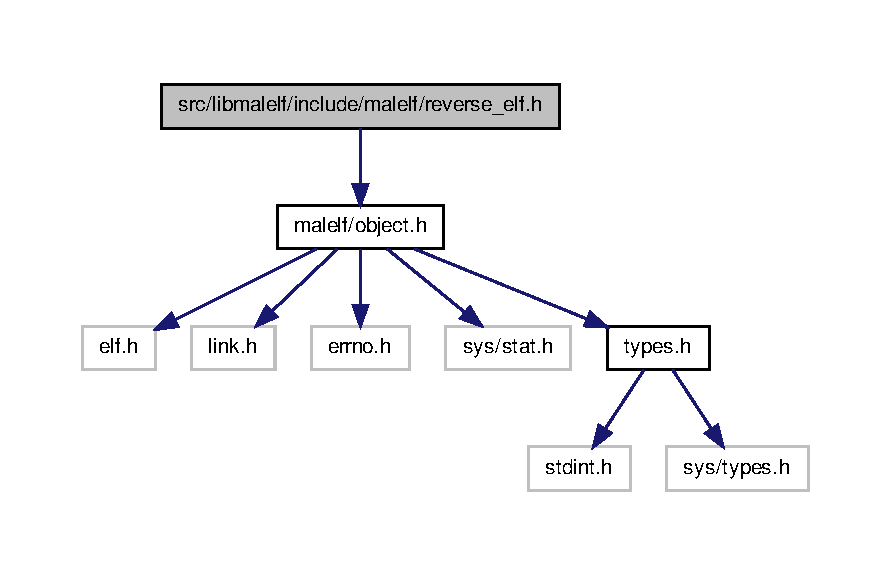
\includegraphics[width=400pt]{reverse__elf_8h__incl}
\end{center}
\end{figure}
This graph shows which files directly or indirectly include this file:\nopagebreak
\begin{figure}[H]
\begin{center}
\leavevmode
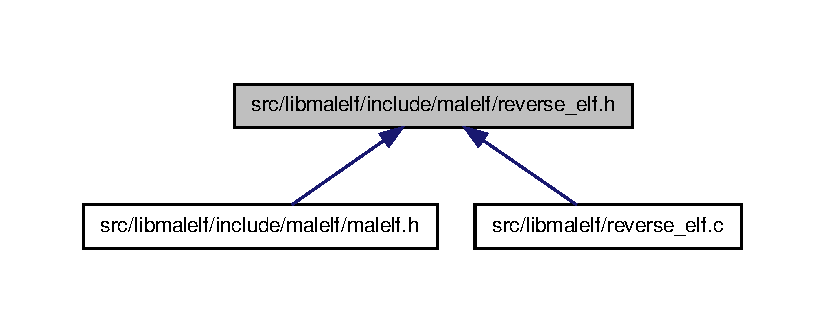
\includegraphics[width=396pt]{reverse__elf_8h__dep__incl}
\end{center}
\end{figure}
\subsection*{Functions}
\begin{DoxyCompactItemize}
\item 
\hyperlink{types_8h_af2b0f13cffd24f6dddf794ae0c7472b4}{\_\-u8} \hyperlink{reverse__elf_8h_af105815abb941024cdf0c799b399ff91}{reverse\_\-elf2c} (\hyperlink{structmalelf__object}{malelf\_\-object} $\ast$elf, FILE $\ast$fd)
\end{DoxyCompactItemize}


\subsection{Function Documentation}
\hypertarget{reverse__elf_8h_af105815abb941024cdf0c799b399ff91}{
\index{reverse\_\-elf.h@{reverse\_\-elf.h}!reverse\_\-elf2c@{reverse\_\-elf2c}}
\index{reverse\_\-elf2c@{reverse\_\-elf2c}!reverse_elf.h@{reverse\_\-elf.h}}
\subsubsection[{reverse\_\-elf2c}]{\setlength{\rightskip}{0pt plus 5cm}{\bf \_\-u8} reverse\_\-elf2c (
\begin{DoxyParamCaption}
\item[{{\bf malelf\_\-object} $\ast$}]{elf, }
\item[{FILE $\ast$}]{fd}
\end{DoxyParamCaption}
)}}
\label{reverse__elf_8h_af105815abb941024cdf0c799b399ff91}


Definition at line 120 of file reverse\_\-elf.c.


\hypertarget{shellcode_8h}{
\section{src/libmalelf/include/malelf/shellcode.h File Reference}
\label{shellcode_8h}\index{src/libmalelf/include/malelf/shellcode.h@{src/libmalelf/include/malelf/shellcode.h}}
}
This graph shows which files directly or indirectly include this file:\nopagebreak
\begin{figure}[H]
\begin{center}
\leavevmode
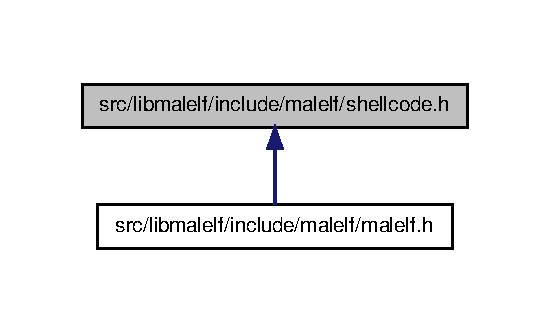
\includegraphics[width=264pt]{shellcode_8h__dep__incl}
\end{center}
\end{figure}
\subsection*{Functions}
\begin{DoxyCompactItemize}
\item 
int \hyperlink{shellcode_8h_aeb967a3ddc1586f237ce4f150327f74a}{shellcode\_\-create\_\-c} (FILE $\ast$fd\_\-o, int in\_\-size, FILE $\ast$fd\_\-i, unsigned long int original\_\-entry\_\-point)
\item 
int \hyperlink{shellcode_8h_a2c56f6b0315593dcb61fcea5ac693d98}{shellcode\_\-create\_\-malelficus} (FILE $\ast$fd\_\-o, int in\_\-size, FILE $\ast$fd\_\-i, unsigned long int original\_\-entry\_\-point, unsigned long int magic\_\-bytes)
\end{DoxyCompactItemize}


\subsection{Function Documentation}
\hypertarget{shellcode_8h_aeb967a3ddc1586f237ce4f150327f74a}{
\index{shellcode.h@{shellcode.h}!shellcode\_\-create\_\-c@{shellcode\_\-create\_\-c}}
\index{shellcode\_\-create\_\-c@{shellcode\_\-create\_\-c}!shellcode.h@{shellcode.h}}
\subsubsection[{shellcode\_\-create\_\-c}]{\setlength{\rightskip}{0pt plus 5cm}int shellcode\_\-create\_\-c (
\begin{DoxyParamCaption}
\item[{FILE $\ast$}]{fd\_\-o, }
\item[{int}]{in\_\-size, }
\item[{FILE $\ast$}]{fd\_\-i, }
\item[{unsigned long int}]{original\_\-entry\_\-point}
\end{DoxyParamCaption}
)}}
\label{shellcode_8h_aeb967a3ddc1586f237ce4f150327f74a}


Definition at line 59 of file shellcode.c.

\hypertarget{shellcode_8h_a2c56f6b0315593dcb61fcea5ac693d98}{
\index{shellcode.h@{shellcode.h}!shellcode\_\-create\_\-malelficus@{shellcode\_\-create\_\-malelficus}}
\index{shellcode\_\-create\_\-malelficus@{shellcode\_\-create\_\-malelficus}!shellcode.h@{shellcode.h}}
\subsubsection[{shellcode\_\-create\_\-malelficus}]{\setlength{\rightskip}{0pt plus 5cm}int shellcode\_\-create\_\-malelficus (
\begin{DoxyParamCaption}
\item[{FILE $\ast$}]{fd\_\-o, }
\item[{int}]{in\_\-size, }
\item[{FILE $\ast$}]{fd\_\-i, }
\item[{unsigned long int}]{original\_\-entry\_\-point, }
\item[{unsigned long int}]{magic\_\-bytes}
\end{DoxyParamCaption}
)}}
\label{shellcode_8h_a2c56f6b0315593dcb61fcea5ac693d98}


Definition at line 16 of file shellcode.c.


\hypertarget{types_8h}{
\section{src/libmalelf/include/malelf/types.h File Reference}
\label{types_8h}\index{src/libmalelf/include/malelf/types.h@{src/libmalelf/include/malelf/types.h}}
}
{\ttfamily \#include $<$stdint.h$>$}\par
{\ttfamily \#include $<$sys/types.h$>$}\par
Include dependency graph for types.h:\nopagebreak
\begin{figure}[H]
\begin{center}
\leavevmode
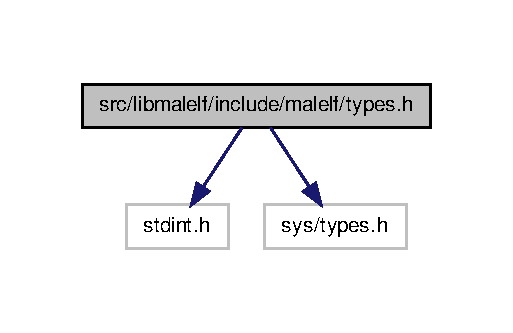
\includegraphics[width=246pt]{types_8h__incl}
\end{center}
\end{figure}
This graph shows which files directly or indirectly include this file:\nopagebreak
\begin{figure}[H]
\begin{center}
\leavevmode
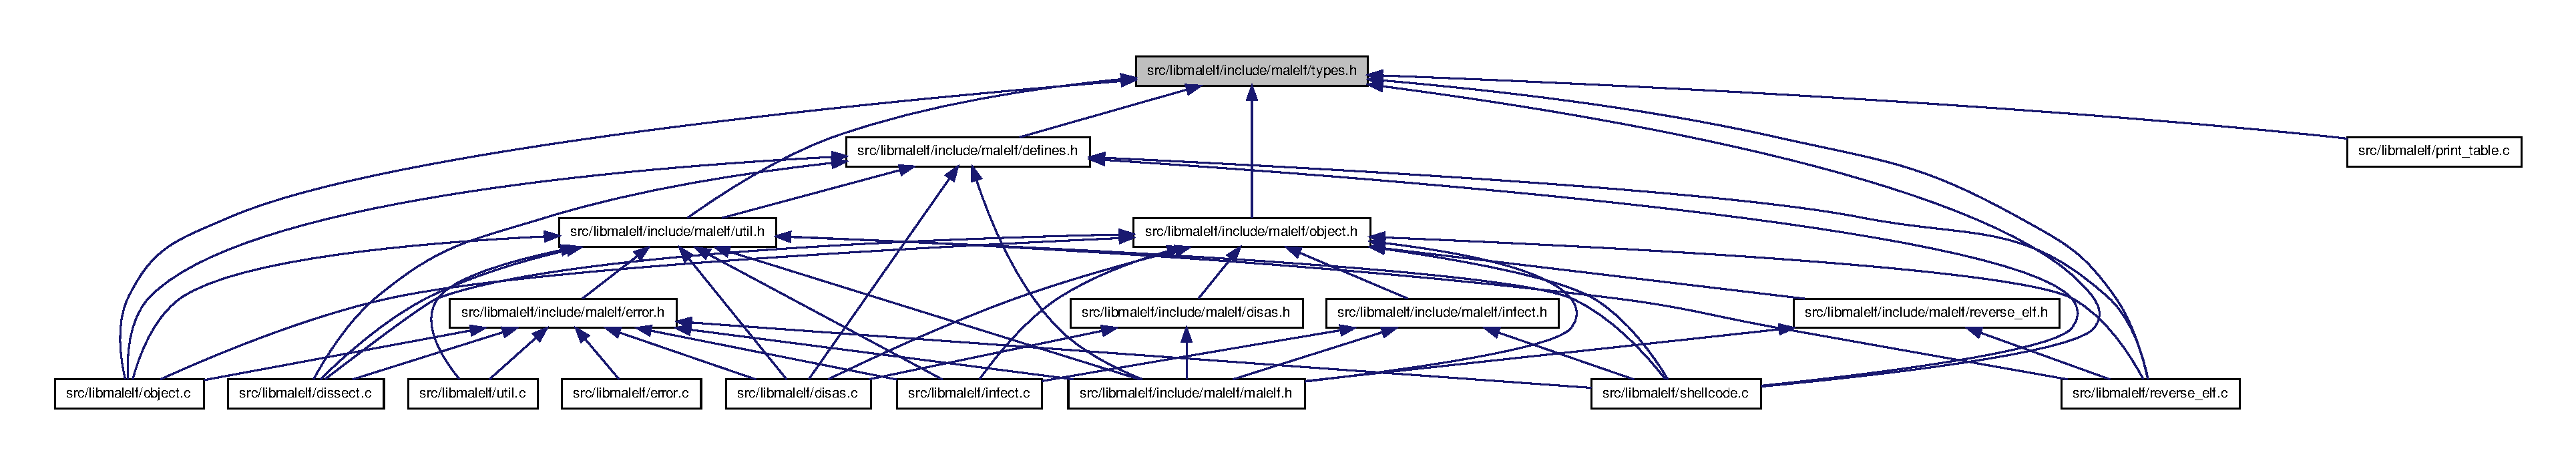
\includegraphics[width=400pt]{types_8h__dep__incl}
\end{center}
\end{figure}
\subsection*{Classes}
\begin{DoxyCompactItemize}
\item 
struct \hyperlink{structmalelf__dissect__opt}{malelf\_\-dissect\_\-opt}
\end{DoxyCompactItemize}
\subsection*{Typedefs}
\begin{DoxyCompactItemize}
\item 
typedef uint8\_\-t \hyperlink{types_8h_af2b0f13cffd24f6dddf794ae0c7472b4}{\_\-u8}
\item 
typedef uint16\_\-t \hyperlink{types_8h_a0ff807843ee3edd61b33fa0425b571e6}{\_\-u16}
\item 
typedef uint32\_\-t \hyperlink{types_8h_a07491c35a48354e0e7b56974a04cc3de}{\_\-u32}
\item 
typedef int8\_\-t \hyperlink{types_8h_a045065388d2a28399f4eae010e4e2582}{\_\-i8}
\item 
typedef int16\_\-t \hyperlink{types_8h_a73ed71cd7860852160f366656f2d1e23}{\_\-i16}
\item 
typedef int32\_\-t \hyperlink{types_8h_aacb1ea6e27efde1c708a8bc4b56ee1a2}{\_\-i32}
\end{DoxyCompactItemize}


\subsection{Typedef Documentation}
\hypertarget{types_8h_a73ed71cd7860852160f366656f2d1e23}{
\index{types.h@{types.h}!\_\-i16@{\_\-i16}}
\index{\_\-i16@{\_\-i16}!types.h@{types.h}}
\subsubsection[{\_\-i16}]{\setlength{\rightskip}{0pt plus 5cm}typedef int16\_\-t {\bf \_\-i16}}}
\label{types_8h_a73ed71cd7860852160f366656f2d1e23}


Definition at line 11 of file types.h.

\hypertarget{types_8h_aacb1ea6e27efde1c708a8bc4b56ee1a2}{
\index{types.h@{types.h}!\_\-i32@{\_\-i32}}
\index{\_\-i32@{\_\-i32}!types.h@{types.h}}
\subsubsection[{\_\-i32}]{\setlength{\rightskip}{0pt plus 5cm}typedef int32\_\-t {\bf \_\-i32}}}
\label{types_8h_aacb1ea6e27efde1c708a8bc4b56ee1a2}


Definition at line 12 of file types.h.

\hypertarget{types_8h_a045065388d2a28399f4eae010e4e2582}{
\index{types.h@{types.h}!\_\-i8@{\_\-i8}}
\index{\_\-i8@{\_\-i8}!types.h@{types.h}}
\subsubsection[{\_\-i8}]{\setlength{\rightskip}{0pt plus 5cm}typedef int8\_\-t {\bf \_\-i8}}}
\label{types_8h_a045065388d2a28399f4eae010e4e2582}


Definition at line 10 of file types.h.

\hypertarget{types_8h_a0ff807843ee3edd61b33fa0425b571e6}{
\index{types.h@{types.h}!\_\-u16@{\_\-u16}}
\index{\_\-u16@{\_\-u16}!types.h@{types.h}}
\subsubsection[{\_\-u16}]{\setlength{\rightskip}{0pt plus 5cm}typedef uint16\_\-t {\bf \_\-u16}}}
\label{types_8h_a0ff807843ee3edd61b33fa0425b571e6}


Definition at line 8 of file types.h.

\hypertarget{types_8h_a07491c35a48354e0e7b56974a04cc3de}{
\index{types.h@{types.h}!\_\-u32@{\_\-u32}}
\index{\_\-u32@{\_\-u32}!types.h@{types.h}}
\subsubsection[{\_\-u32}]{\setlength{\rightskip}{0pt plus 5cm}typedef uint32\_\-t {\bf \_\-u32}}}
\label{types_8h_a07491c35a48354e0e7b56974a04cc3de}


Definition at line 9 of file types.h.

\hypertarget{types_8h_af2b0f13cffd24f6dddf794ae0c7472b4}{
\index{types.h@{types.h}!\_\-u8@{\_\-u8}}
\index{\_\-u8@{\_\-u8}!types.h@{types.h}}
\subsubsection[{\_\-u8}]{\setlength{\rightskip}{0pt plus 5cm}typedef uint8\_\-t {\bf \_\-u8}}}
\label{types_8h_af2b0f13cffd24f6dddf794ae0c7472b4}


Definition at line 7 of file types.h.


\hypertarget{util_8h}{
\section{src/libmalelf/include/malelf/util.h File Reference}
\label{util_8h}\index{src/libmalelf/include/malelf/util.h@{src/libmalelf/include/malelf/util.h}}
}
{\ttfamily \#include $<$stdio.h$>$}\par
{\ttfamily \#include $<$stdarg.h$>$}\par
{\ttfamily \#include \char`\"{}defines.h\char`\"{}}\par
{\ttfamily \#include \char`\"{}types.h\char`\"{}}\par
Include dependency graph for util.h:\nopagebreak
\begin{figure}[H]
\begin{center}
\leavevmode
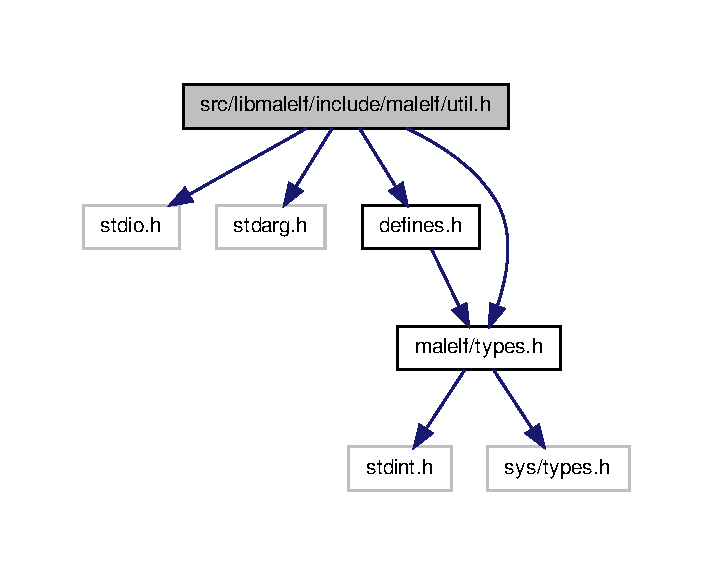
\includegraphics[width=342pt]{util_8h__incl}
\end{center}
\end{figure}
This graph shows which files directly or indirectly include this file:\nopagebreak
\begin{figure}[H]
\begin{center}
\leavevmode
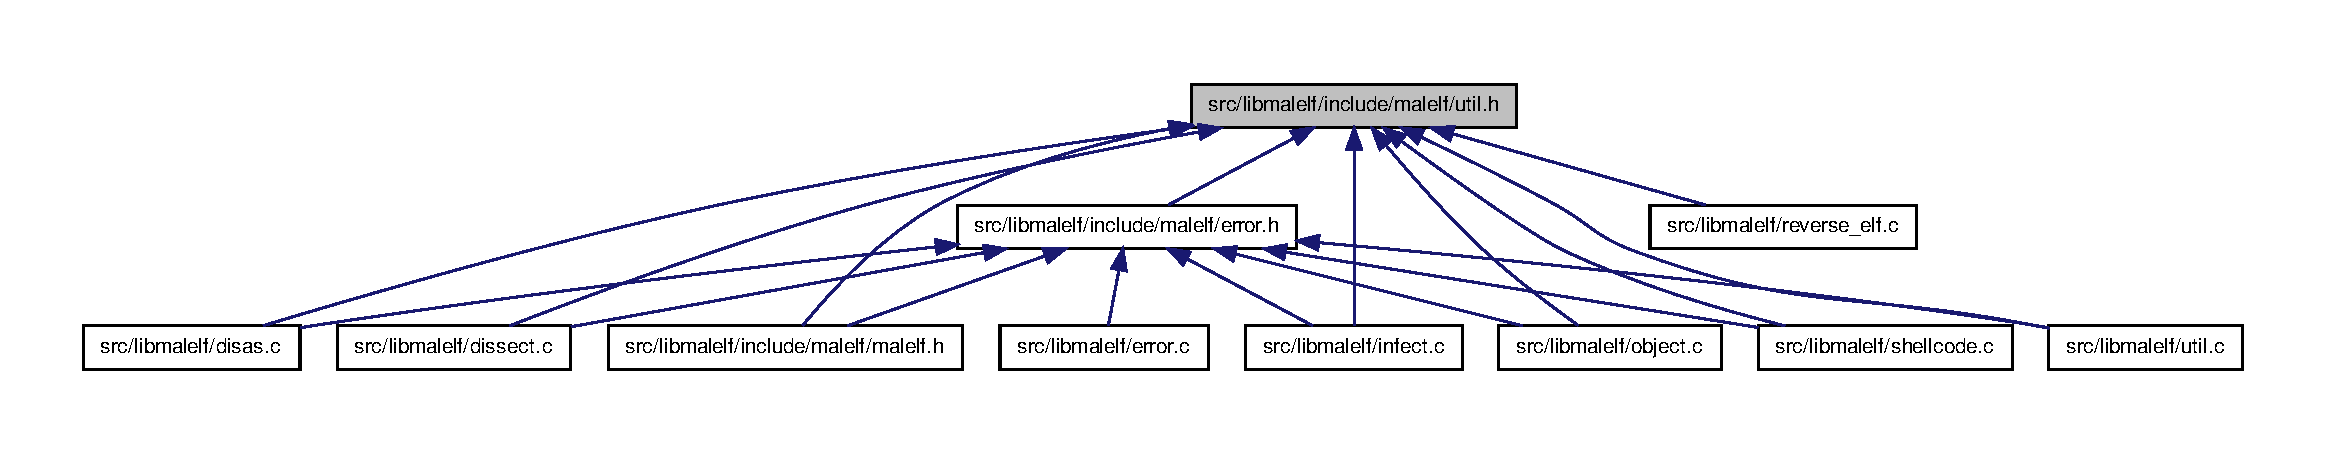
\includegraphics[width=400pt]{util_8h__dep__incl}
\end{center}
\end{figure}
\subsection*{Defines}
\begin{DoxyCompactItemize}
\item 
\#define \hyperlink{util_8h_a12dc04e9161abfdd033e2bb0193e6387}{MAX\_\-LOG\_\-BUFFER}~1024
\item 
\#define \hyperlink{util_8h_ad949df569bf250c13a2b0afb4202c788}{LOG\_\-RAW}~malelf\_\-say
\item 
\#define \hyperlink{util_8h_aaa5f65974d3240c5828344f78cebde50}{SAY}~if(!\hyperlink{util_8c_a9832bf9a14bd3b9656e7be172ac16c9b}{malelf\_\-quiet\_\-mode}) malelf\_\-say
\item 
\#define \hyperlink{util_8h_a159ca84d25a5487d8e81e4438725df19}{LOG}~LOG\_\-RAW
\item 
\#define \hyperlink{util_8h_a41a95f9112ce515b554571d40c926251}{LOG\_\-SUCCESS}~if (!\hyperlink{util_8c_a9832bf9a14bd3b9656e7be172ac16c9b}{malelf\_\-quiet\_\-mode}) malelf\_\-success
\item 
\#define \hyperlink{util_8h_adf8c5c50672d8ac8c77490e507611618}{LOG\_\-VERBOSE\_\-SUCCESS}~if (\hyperlink{defines_8h_acd6ab4d02330caecbb7e6e11930b31b3}{malelf\_\-verbose\_\-mode}) LOG\_\-SUCCESS
\item 
\#define \hyperlink{util_8h_aced66975c154ea0e2a8ec3bc818b4e08}{LOG\_\-ERROR}~if (!\hyperlink{util_8c_a9832bf9a14bd3b9656e7be172ac16c9b}{malelf\_\-quiet\_\-mode}) malelf\_\-error
\item 
\#define \hyperlink{util_8h_aea3f57d6dcc5b4ac957e2679e87dde27}{LOG\_\-WARN}~malelf\_\-warn
\item 
\#define \hyperlink{util_8h_aadf6774e19887211734c54a45c3dd171}{LOG\_\-OFFSET}(desc\_\-format, value)
\item 
\#define \hyperlink{util_8h_ac4ac9f31cfaaefb4f69098bb1d4c3735}{ITOA}(dest, src)~sprintf(dest, \char`\"{}\%d\char`\"{}, src)
\item 
\#define \hyperlink{util_8h_a93cbdd21c4ca66a81684b4aef7dcbdf7}{HTOA}(dest, src)~sprintf(dest, \char`\"{}0x\%08x\char`\"{}, src)
\item 
\#define \hyperlink{util_8h_ac87d3b54aa4120dcc7d3bc368e8ecfa7}{MALELF\_\-UNUSED}(var)~(void$\ast$)var
\end{DoxyCompactItemize}
\subsection*{Functions}
\begin{DoxyCompactItemize}
\item 
\hyperlink{types_8h_af2b0f13cffd24f6dddf794ae0c7472b4}{\_\-u8} \hyperlink{util_8h_a7030062f94da236e11cadbd65d7a2c29}{saveFile} (const char $\ast$fname, \hyperlink{types_8h_af2b0f13cffd24f6dddf794ae0c7472b4}{\_\-u8} $\ast$mem, off\_\-t size)
\item 
int \hyperlink{util_8h_a247542ae0b6acc9ada0109283141c737}{malelf\_\-log} (FILE $\ast$fd, const char $\ast$prefix, const char $\ast$format, va\_\-list args)
\item 
int \hyperlink{util_8h_ac6734a7443633a78f6a87d5511ca2364}{malelf\_\-print} (FILE $\ast$fd, const char $\ast$format,...)
\item 
int \hyperlink{util_8h_a1cd6a5086679cbb2b107e781aeb3835d}{malelf\_\-say} (const char $\ast$format,...)
\item 
int \hyperlink{util_8h_aea4d2b93d2acad2b43abc0aff8680828}{malelf\_\-success} (const char $\ast$format,...)
\item 
int \hyperlink{util_8h_a9d6a039b287860279870f4297d80ef6a}{malelf\_\-error} (const char $\ast$format,...)
\item 
int \hyperlink{util_8h_abf9a0a02da3599092c0aa5cbbe62ff2f}{malelf\_\-warn} (const char $\ast$format,...)
\end{DoxyCompactItemize}


\subsection{Define Documentation}
\hypertarget{util_8h_a93cbdd21c4ca66a81684b4aef7dcbdf7}{
\index{util.h@{util.h}!HTOA@{HTOA}}
\index{HTOA@{HTOA}!util.h@{util.h}}
\subsubsection[{HTOA}]{\setlength{\rightskip}{0pt plus 5cm}\#define HTOA(
\begin{DoxyParamCaption}
\item[{}]{dest, }
\item[{}]{src}
\end{DoxyParamCaption}
)~sprintf(dest, \char`\"{}0x\%08x\char`\"{}, src)}}
\label{util_8h_a93cbdd21c4ca66a81684b4aef7dcbdf7}


Definition at line 27 of file util.h.

\hypertarget{util_8h_ac4ac9f31cfaaefb4f69098bb1d4c3735}{
\index{util.h@{util.h}!ITOA@{ITOA}}
\index{ITOA@{ITOA}!util.h@{util.h}}
\subsubsection[{ITOA}]{\setlength{\rightskip}{0pt plus 5cm}\#define ITOA(
\begin{DoxyParamCaption}
\item[{}]{dest, }
\item[{}]{src}
\end{DoxyParamCaption}
)~sprintf(dest, \char`\"{}\%d\char`\"{}, src)}}
\label{util_8h_ac4ac9f31cfaaefb4f69098bb1d4c3735}


Definition at line 26 of file util.h.

\hypertarget{util_8h_a159ca84d25a5487d8e81e4438725df19}{
\index{util.h@{util.h}!LOG@{LOG}}
\index{LOG@{LOG}!util.h@{util.h}}
\subsubsection[{LOG}]{\setlength{\rightskip}{0pt plus 5cm}\#define LOG~LOG\_\-RAW}}
\label{util_8h_a159ca84d25a5487d8e81e4438725df19}


Definition at line 16 of file util.h.

\hypertarget{util_8h_aced66975c154ea0e2a8ec3bc818b4e08}{
\index{util.h@{util.h}!LOG\_\-ERROR@{LOG\_\-ERROR}}
\index{LOG\_\-ERROR@{LOG\_\-ERROR}!util.h@{util.h}}
\subsubsection[{LOG\_\-ERROR}]{\setlength{\rightskip}{0pt plus 5cm}\#define LOG\_\-ERROR~if (!{\bf malelf\_\-quiet\_\-mode}) malelf\_\-error}}
\label{util_8h_aced66975c154ea0e2a8ec3bc818b4e08}


Definition at line 19 of file util.h.

\hypertarget{util_8h_aadf6774e19887211734c54a45c3dd171}{
\index{util.h@{util.h}!LOG\_\-OFFSET@{LOG\_\-OFFSET}}
\index{LOG\_\-OFFSET@{LOG\_\-OFFSET}!util.h@{util.h}}
\subsubsection[{LOG\_\-OFFSET}]{\setlength{\rightskip}{0pt plus 5cm}\#define LOG\_\-OFFSET(
\begin{DoxyParamCaption}
\item[{}]{desc\_\-format, }
\item[{}]{value}
\end{DoxyParamCaption}
)}}
\label{util_8h_aadf6774e19887211734c54a45c3dd171}
{\bfseries Value:}
\begin{DoxyCode}
if (malelf_quiet_mode) {                             \
    LOG_RAW("0x%x", value);                     \
  } else LOG_RAW(desc_format, value)
\end{DoxyCode}


Definition at line 21 of file util.h.

\hypertarget{util_8h_ad949df569bf250c13a2b0afb4202c788}{
\index{util.h@{util.h}!LOG\_\-RAW@{LOG\_\-RAW}}
\index{LOG\_\-RAW@{LOG\_\-RAW}!util.h@{util.h}}
\subsubsection[{LOG\_\-RAW}]{\setlength{\rightskip}{0pt plus 5cm}\#define LOG\_\-RAW~malelf\_\-say}}
\label{util_8h_ad949df569bf250c13a2b0afb4202c788}
Macros 

Definition at line 14 of file util.h.

\hypertarget{util_8h_a41a95f9112ce515b554571d40c926251}{
\index{util.h@{util.h}!LOG\_\-SUCCESS@{LOG\_\-SUCCESS}}
\index{LOG\_\-SUCCESS@{LOG\_\-SUCCESS}!util.h@{util.h}}
\subsubsection[{LOG\_\-SUCCESS}]{\setlength{\rightskip}{0pt plus 5cm}\#define LOG\_\-SUCCESS~if (!{\bf malelf\_\-quiet\_\-mode}) malelf\_\-success}}
\label{util_8h_a41a95f9112ce515b554571d40c926251}


Definition at line 17 of file util.h.

\hypertarget{util_8h_adf8c5c50672d8ac8c77490e507611618}{
\index{util.h@{util.h}!LOG\_\-VERBOSE\_\-SUCCESS@{LOG\_\-VERBOSE\_\-SUCCESS}}
\index{LOG\_\-VERBOSE\_\-SUCCESS@{LOG\_\-VERBOSE\_\-SUCCESS}!util.h@{util.h}}
\subsubsection[{LOG\_\-VERBOSE\_\-SUCCESS}]{\setlength{\rightskip}{0pt plus 5cm}\#define LOG\_\-VERBOSE\_\-SUCCESS~if ({\bf malelf\_\-verbose\_\-mode}) LOG\_\-SUCCESS}}
\label{util_8h_adf8c5c50672d8ac8c77490e507611618}


Definition at line 18 of file util.h.

\hypertarget{util_8h_aea3f57d6dcc5b4ac957e2679e87dde27}{
\index{util.h@{util.h}!LOG\_\-WARN@{LOG\_\-WARN}}
\index{LOG\_\-WARN@{LOG\_\-WARN}!util.h@{util.h}}
\subsubsection[{LOG\_\-WARN}]{\setlength{\rightskip}{0pt plus 5cm}\#define LOG\_\-WARN~malelf\_\-warn}}
\label{util_8h_aea3f57d6dcc5b4ac957e2679e87dde27}


Definition at line 20 of file util.h.

\hypertarget{util_8h_ac87d3b54aa4120dcc7d3bc368e8ecfa7}{
\index{util.h@{util.h}!MALELF\_\-UNUSED@{MALELF\_\-UNUSED}}
\index{MALELF\_\-UNUSED@{MALELF\_\-UNUSED}!util.h@{util.h}}
\subsubsection[{MALELF\_\-UNUSED}]{\setlength{\rightskip}{0pt plus 5cm}\#define MALELF\_\-UNUSED(
\begin{DoxyParamCaption}
\item[{}]{var}
\end{DoxyParamCaption}
)~(void$\ast$)var}}
\label{util_8h_ac87d3b54aa4120dcc7d3bc368e8ecfa7}


Definition at line 29 of file util.h.

\hypertarget{util_8h_a12dc04e9161abfdd033e2bb0193e6387}{
\index{util.h@{util.h}!MAX\_\-LOG\_\-BUFFER@{MAX\_\-LOG\_\-BUFFER}}
\index{MAX\_\-LOG\_\-BUFFER@{MAX\_\-LOG\_\-BUFFER}!util.h@{util.h}}
\subsubsection[{MAX\_\-LOG\_\-BUFFER}]{\setlength{\rightskip}{0pt plus 5cm}\#define MAX\_\-LOG\_\-BUFFER~1024}}
\label{util_8h_a12dc04e9161abfdd033e2bb0193e6387}


Definition at line 9 of file util.h.

\hypertarget{util_8h_aaa5f65974d3240c5828344f78cebde50}{
\index{util.h@{util.h}!SAY@{SAY}}
\index{SAY@{SAY}!util.h@{util.h}}
\subsubsection[{SAY}]{\setlength{\rightskip}{0pt plus 5cm}\#define SAY~if(!{\bf malelf\_\-quiet\_\-mode}) malelf\_\-say}}
\label{util_8h_aaa5f65974d3240c5828344f78cebde50}


Definition at line 15 of file util.h.



\subsection{Function Documentation}
\hypertarget{util_8h_a9d6a039b287860279870f4297d80ef6a}{
\index{util.h@{util.h}!malelf\_\-error@{malelf\_\-error}}
\index{malelf\_\-error@{malelf\_\-error}!util.h@{util.h}}
\subsubsection[{malelf\_\-error}]{\setlength{\rightskip}{0pt plus 5cm}int malelf\_\-error (
\begin{DoxyParamCaption}
\item[{const char $\ast$}]{format, }
\item[{}]{...}
\end{DoxyParamCaption}
)}}
\label{util_8h_a9d6a039b287860279870f4297d80ef6a}


Definition at line 49 of file util.c.

\hypertarget{util_8h_a247542ae0b6acc9ada0109283141c737}{
\index{util.h@{util.h}!malelf\_\-log@{malelf\_\-log}}
\index{malelf\_\-log@{malelf\_\-log}!util.h@{util.h}}
\subsubsection[{malelf\_\-log}]{\setlength{\rightskip}{0pt plus 5cm}int malelf\_\-log (
\begin{DoxyParamCaption}
\item[{FILE $\ast$}]{fd, }
\item[{const char $\ast$}]{prefix, }
\item[{const char $\ast$}]{format, }
\item[{va\_\-list}]{args}
\end{DoxyParamCaption}
)}}
\label{util_8h_a247542ae0b6acc9ada0109283141c737}


Definition at line 15 of file util.c.

\hypertarget{util_8h_ac6734a7443633a78f6a87d5511ca2364}{
\index{util.h@{util.h}!malelf\_\-print@{malelf\_\-print}}
\index{malelf\_\-print@{malelf\_\-print}!util.h@{util.h}}
\subsubsection[{malelf\_\-print}]{\setlength{\rightskip}{0pt plus 5cm}int malelf\_\-print (
\begin{DoxyParamCaption}
\item[{FILE $\ast$}]{fd, }
\item[{const char $\ast$}]{format, }
\item[{}]{...}
\end{DoxyParamCaption}
)}}
\label{util_8h_ac6734a7443633a78f6a87d5511ca2364}


Definition at line 37 of file util.c.

\hypertarget{util_8h_a1cd6a5086679cbb2b107e781aeb3835d}{
\index{util.h@{util.h}!malelf\_\-say@{malelf\_\-say}}
\index{malelf\_\-say@{malelf\_\-say}!util.h@{util.h}}
\subsubsection[{malelf\_\-say}]{\setlength{\rightskip}{0pt plus 5cm}int malelf\_\-say (
\begin{DoxyParamCaption}
\item[{const char $\ast$}]{format, }
\item[{}]{...}
\end{DoxyParamCaption}
)}}
\label{util_8h_a1cd6a5086679cbb2b107e781aeb3835d}


Definition at line 43 of file util.c.

\hypertarget{util_8h_aea4d2b93d2acad2b43abc0aff8680828}{
\index{util.h@{util.h}!malelf\_\-success@{malelf\_\-success}}
\index{malelf\_\-success@{malelf\_\-success}!util.h@{util.h}}
\subsubsection[{malelf\_\-success}]{\setlength{\rightskip}{0pt plus 5cm}int malelf\_\-success (
\begin{DoxyParamCaption}
\item[{const char $\ast$}]{format, }
\item[{}]{...}
\end{DoxyParamCaption}
)}}
\label{util_8h_aea4d2b93d2acad2b43abc0aff8680828}


Definition at line 55 of file util.c.

\hypertarget{util_8h_abf9a0a02da3599092c0aa5cbbe62ff2f}{
\index{util.h@{util.h}!malelf\_\-warn@{malelf\_\-warn}}
\index{malelf\_\-warn@{malelf\_\-warn}!util.h@{util.h}}
\subsubsection[{malelf\_\-warn}]{\setlength{\rightskip}{0pt plus 5cm}int malelf\_\-warn (
\begin{DoxyParamCaption}
\item[{const char $\ast$}]{format, }
\item[{}]{...}
\end{DoxyParamCaption}
)}}
\label{util_8h_abf9a0a02da3599092c0aa5cbbe62ff2f}


Definition at line 61 of file util.c.

\hypertarget{util_8h_a7030062f94da236e11cadbd65d7a2c29}{
\index{util.h@{util.h}!saveFile@{saveFile}}
\index{saveFile@{saveFile}!util.h@{util.h}}
\subsubsection[{saveFile}]{\setlength{\rightskip}{0pt plus 5cm}{\bf \_\-u8} saveFile (
\begin{DoxyParamCaption}
\item[{const char $\ast$}]{fname, }
\item[{{\bf \_\-u8} $\ast$}]{mem, }
\item[{off\_\-t}]{size}
\end{DoxyParamCaption}
)}}
\label{util_8h_a7030062f94da236e11cadbd65d7a2c29}


Definition at line 67 of file util.c.


\hypertarget{infect_8c}{
\section{src/libmalelf/infect.c File Reference}
\label{infect_8c}\index{src/libmalelf/infect.c@{src/libmalelf/infect.c}}
}
{\ttfamily \#include $<$stdio.h$>$}\par
{\ttfamily \#include $<$stdlib.h$>$}\par
{\ttfamily \#include $<$sys/types.h$>$}\par
{\ttfamily \#include $<$sys/stat.h$>$}\par
{\ttfamily \#include $<$unistd.h$>$}\par
{\ttfamily \#include \char`\"{}malelf/infect.h\char`\"{}}\par
{\ttfamily \#include \char`\"{}malelf/util.h\char`\"{}}\par
{\ttfamily \#include \char`\"{}malelf/error.h\char`\"{}}\par
{\ttfamily \#include \char`\"{}malelf/object.h\char`\"{}}\par
Include dependency graph for infect.c:\nopagebreak
\begin{figure}[H]
\begin{center}
\leavevmode
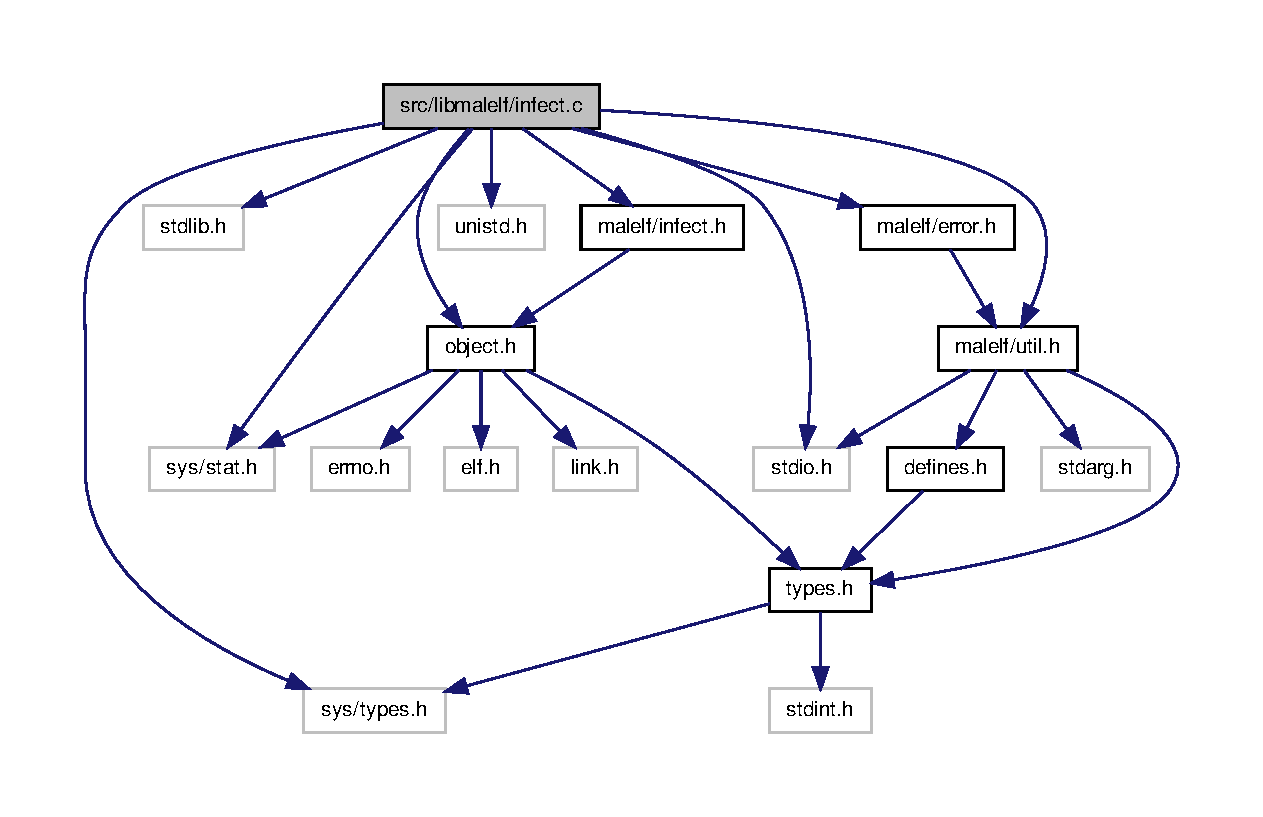
\includegraphics[width=400pt]{infect_8c__incl}
\end{center}
\end{figure}
\subsection*{Defines}
\begin{DoxyCompactItemize}
\item 
\#define \hyperlink{infect_8c_a7d467c1d283fdfa1f2081ba1e0d01b6e}{PAGE\_\-SIZE}~4096
\end{DoxyCompactItemize}
\subsection*{Functions}
\begin{DoxyCompactItemize}
\item 
\hyperlink{types_8h_af2b0f13cffd24f6dddf794ae0c7472b4}{\_\-u8} \hyperlink{infect_8c_ab2204e6548cea638fdc54fe23b0a2ec0}{malelf\_\-infect\_\-silvio\_\-padding} (\hyperlink{structmalelf__object}{malelf\_\-object} $\ast$input, \hyperlink{structmalelf__object}{malelf\_\-object} $\ast$output, \hyperlink{structmalelf__object}{malelf\_\-object} $\ast$parasite, \hyperlink{types_8h_a07491c35a48354e0e7b56974a04cc3de}{\_\-u32} offset\_\-entry\_\-point, unsigned long int magic\_\-bytes)
\item 
\hyperlink{types_8h_af2b0f13cffd24f6dddf794ae0c7472b4}{\_\-u8} \hyperlink{infect_8c_ade77317192a56215582fdb0ad3b44cc6}{\_\-malelf\_\-parasite\_\-silvio\_\-padding} (\hyperlink{structmalelf__object}{malelf\_\-object} $\ast$input, \hyperlink{structmalelf__object}{malelf\_\-object} $\ast$output, unsigned int end\_\-of\_\-text, \hyperlink{structmalelf__object}{malelf\_\-object} $\ast$parasite, \hyperlink{types_8h_a07491c35a48354e0e7b56974a04cc3de}{\_\-u32} offset\_\-entry\_\-point, unsigned old\_\-e\_\-entry, unsigned long int magic\_\-bytes)
\end{DoxyCompactItemize}


\subsection{Define Documentation}
\hypertarget{infect_8c_a7d467c1d283fdfa1f2081ba1e0d01b6e}{
\index{infect.c@{infect.c}!PAGE\_\-SIZE@{PAGE\_\-SIZE}}
\index{PAGE\_\-SIZE@{PAGE\_\-SIZE}!infect.c@{infect.c}}
\subsubsection[{PAGE\_\-SIZE}]{\setlength{\rightskip}{0pt plus 5cm}\#define PAGE\_\-SIZE~4096}}
\label{infect_8c_a7d467c1d283fdfa1f2081ba1e0d01b6e}


Definition at line 36 of file infect.c.



\subsection{Function Documentation}
\hypertarget{infect_8c_ade77317192a56215582fdb0ad3b44cc6}{
\index{infect.c@{infect.c}!\_\-malelf\_\-parasite\_\-silvio\_\-padding@{\_\-malelf\_\-parasite\_\-silvio\_\-padding}}
\index{\_\-malelf\_\-parasite\_\-silvio\_\-padding@{\_\-malelf\_\-parasite\_\-silvio\_\-padding}!infect.c@{infect.c}}
\subsubsection[{\_\-malelf\_\-parasite\_\-silvio\_\-padding}]{\setlength{\rightskip}{0pt plus 5cm}{\bf \_\-u8} \_\-malelf\_\-parasite\_\-silvio\_\-padding (
\begin{DoxyParamCaption}
\item[{{\bf malelf\_\-object} $\ast$}]{input, }
\item[{{\bf malelf\_\-object} $\ast$}]{output, }
\item[{unsigned int}]{end\_\-of\_\-text, }
\item[{{\bf malelf\_\-object} $\ast$}]{parasite, }
\item[{{\bf \_\-u32}}]{offset\_\-entry\_\-point, }
\item[{unsigned}]{old\_\-e\_\-entry, }
\item[{unsigned long int}]{magic\_\-bytes}
\end{DoxyParamCaption}
)}}
\label{infect_8c_ade77317192a56215582fdb0ad3b44cc6}


Definition at line 135 of file infect.c.

\hypertarget{infect_8c_ab2204e6548cea638fdc54fe23b0a2ec0}{
\index{infect.c@{infect.c}!malelf\_\-infect\_\-silvio\_\-padding@{malelf\_\-infect\_\-silvio\_\-padding}}
\index{malelf\_\-infect\_\-silvio\_\-padding@{malelf\_\-infect\_\-silvio\_\-padding}!infect.c@{infect.c}}
\subsubsection[{malelf\_\-infect\_\-silvio\_\-padding}]{\setlength{\rightskip}{0pt plus 5cm}{\bf \_\-u8} malelf\_\-infect\_\-silvio\_\-padding (
\begin{DoxyParamCaption}
\item[{{\bf malelf\_\-object} $\ast$}]{input, }
\item[{{\bf malelf\_\-object} $\ast$}]{output, }
\item[{{\bf malelf\_\-object} $\ast$}]{parasite, }
\item[{{\bf \_\-u32}}]{offset\_\-entry\_\-point, }
\item[{unsigned long int}]{magic\_\-bytes}
\end{DoxyParamCaption}
)}}
\label{infect_8c_ab2204e6548cea638fdc54fe23b0a2ec0}
Try to infect the ELF using the text padding technique created by Silvio Cesare. More information: \href{http://www.win.tue.nl/~aeb/linux/hh/virus/unix-viruses.txt}{\tt http://www.win.tue.nl/$\sim$aeb/linux/hh/virus/unix-\/viruses.txt} 

Definition at line 43 of file infect.c.


\hypertarget{machines_8inc}{
\section{src/libmalelf/machines.inc File Reference}
\label{machines_8inc}\index{src/libmalelf/machines.inc@{src/libmalelf/machines.inc}}
}
This graph shows which files directly or indirectly include this file:\nopagebreak
\begin{figure}[H]
\begin{center}
\leavevmode
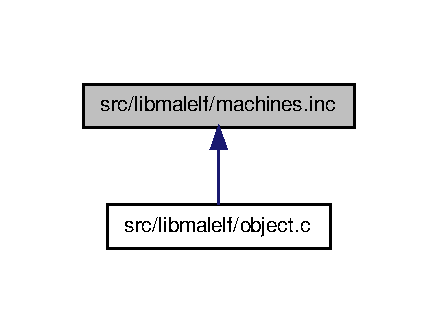
\includegraphics[width=210pt]{machines_8inc__dep__incl}
\end{center}
\end{figure}

\hypertarget{mainpage_8h}{
\section{src/libmalelf/mainpage.h File Reference}
\label{mainpage_8h}\index{src/libmalelf/mainpage.h@{src/libmalelf/mainpage.h}}
}


Definition of class Template.  




\subsection{Detailed Description}
Definition of class Template. \begin{DoxyParagraph}{Header:}
/nfs/slac/g/glast/ground/cvs/workbook/pages/advanced\_\-doxygen/usingDoxygen.htm,v 1.1.1.1 2007/06/29 15:03:16 chuckp Exp 
\end{DoxyParagraph}


Definition in file \hyperlink{mainpage_8h_source}{mainpage.h}.


\hypertarget{object_8c}{
\section{src/libmalelf/object.c File Reference}
\label{object_8c}\index{src/libmalelf/object.c@{src/libmalelf/object.c}}
}
{\ttfamily \#include $<$stdio.h$>$}\par
{\ttfamily \#include $<$stdlib.h$>$}\par
{\ttfamily \#include $<$string.h$>$}\par
{\ttfamily \#include $<$strings.h$>$}\par
{\ttfamily \#include $<$unistd.h$>$}\par
{\ttfamily \#include $<$assert.h$>$}\par
{\ttfamily \#include $<$errno.h$>$}\par
{\ttfamily \#include $<$sys/types.h$>$}\par
{\ttfamily \#include $<$sys/stat.h$>$}\par
{\ttfamily \#include $<$fcntl.h$>$}\par
{\ttfamily \#include $<$sys/mman.h$>$}\par
{\ttfamily \#include $<$malelf/defines.h$>$}\par
{\ttfamily \#include $<$malelf/util.h$>$}\par
{\ttfamily \#include $<$malelf/types.h$>$}\par
{\ttfamily \#include $<$malelf/error.h$>$}\par
{\ttfamily \#include $<$malelf/object.h$>$}\par
{\ttfamily \#include $<$malelf/dissect.h$>$}\par
{\ttfamily \#include \char`\"{}header\_\-types.inc\char`\"{}}\par
{\ttfamily \#include \char`\"{}machines.inc\char`\"{}}\par
{\ttfamily \#include \char`\"{}section\_\-types.inc\char`\"{}}\par
{\ttfamily \#include \char`\"{}segment\_\-types.inc\char`\"{}}\par
{\ttfamily \#include \char`\"{}segment\_\-flags.inc\char`\"{}}\par
Include dependency graph for object.c:\nopagebreak
\begin{figure}[H]
\begin{center}
\leavevmode
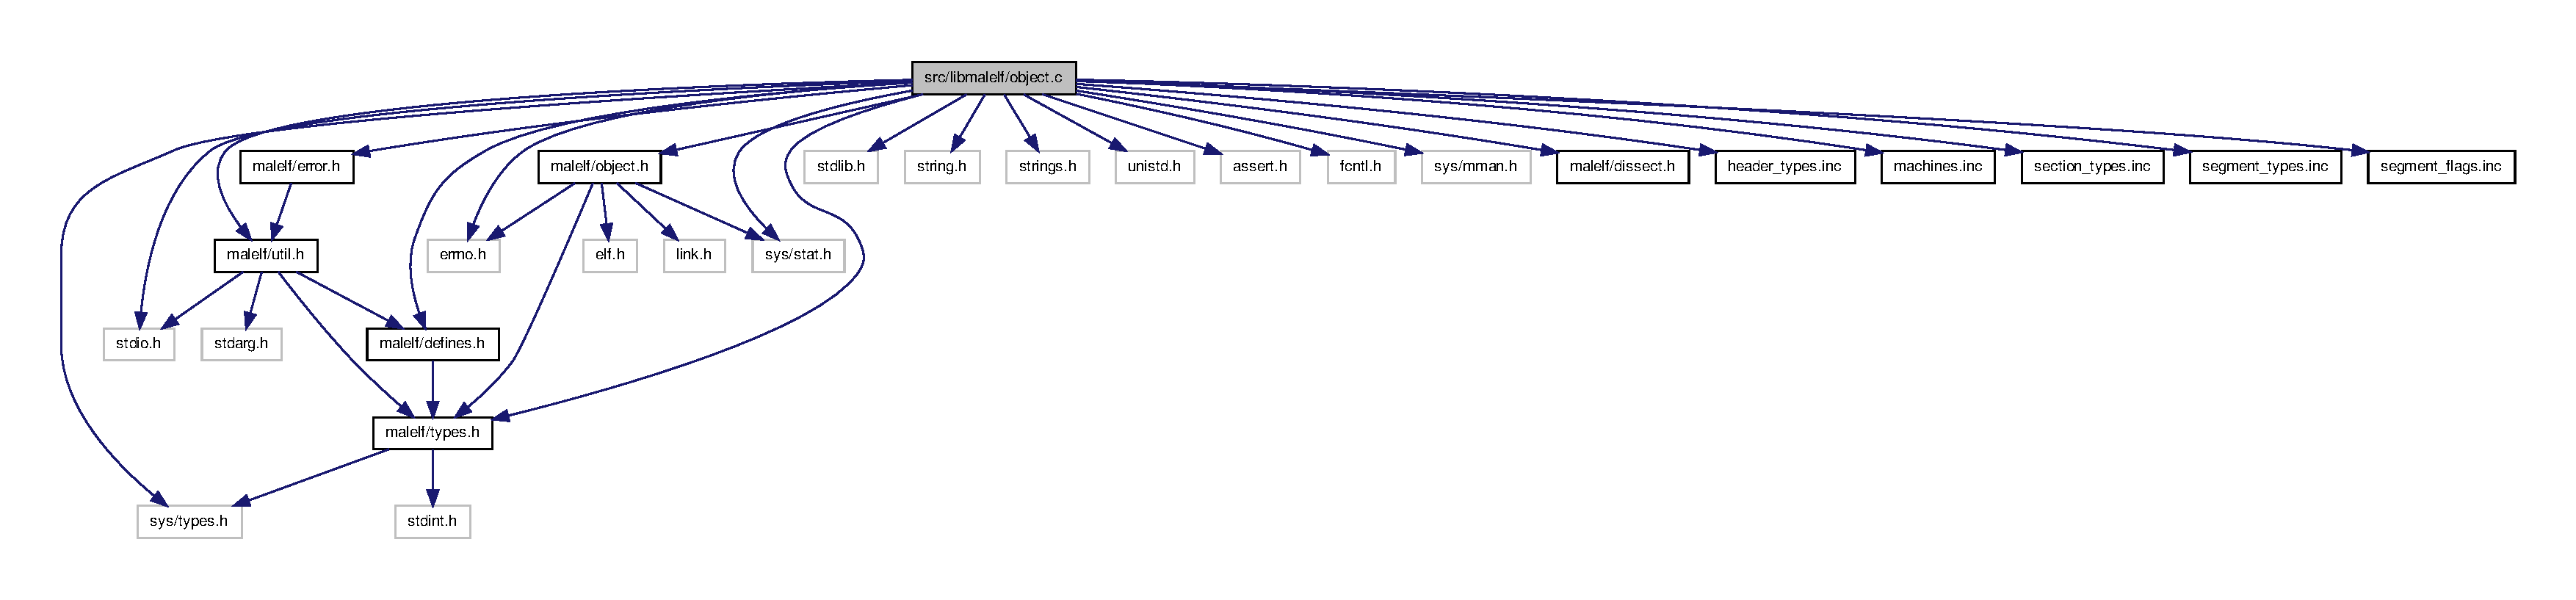
\includegraphics[width=400pt]{object_8c__incl}
\end{center}
\end{figure}
\subsection*{Functions}
\begin{DoxyCompactItemize}
\item 
void \hyperlink{object_8c_a3e207e88c2ed18f5a6851d8685ce43c6}{malelf\_\-init\_\-object} (\hyperlink{structmalelf__object}{malelf\_\-object} $\ast$obj)
\begin{DoxyCompactList}\small\item\em Initialize the malelf object data type. \end{DoxyCompactList}\item 
\hyperlink{types_8h_af2b0f13cffd24f6dddf794ae0c7472b4}{\_\-u8} \hyperlink{object_8c_ab72f2409e093e754523c77367c4d92cf}{malelf\_\-check\_\-elf} (\hyperlink{structmalelf__object}{malelf\_\-object} $\ast$obj)
\begin{DoxyCompactList}\small\item\em Check if the binary file mapped in obj is of type ELF. \end{DoxyCompactList}\item 
\hyperlink{types_8h_aacb1ea6e27efde1c708a8bc4b56ee1a2}{\_\-i32} \hyperlink{object_8c_a54b384361ec6e433175bb58ef217467b}{malelf\_\-open} (\hyperlink{structmalelf__object}{malelf\_\-object} $\ast$obj, char $\ast$filename, int flags)
\begin{DoxyCompactList}\small\item\em Open the binary file 'filename' and fill the struct \hyperlink{structmalelf__object}{malelf\_\-object}. \end{DoxyCompactList}\item 
\hyperlink{types_8h_aacb1ea6e27efde1c708a8bc4b56ee1a2}{\_\-i32} \hyperlink{object_8c_a6daa20f1e4fb72096a9eb27ee0234a85}{malelf\_\-openr} (\hyperlink{structmalelf__object}{malelf\_\-object} $\ast$obj, char $\ast$filename)
\item 
\hyperlink{types_8h_aacb1ea6e27efde1c708a8bc4b56ee1a2}{\_\-i32} \hyperlink{object_8c_a44e74dbe97ac2f3a4571b53cafa3833f}{malelf\_\-openw} (\hyperlink{structmalelf__object}{malelf\_\-object} $\ast$obj, char $\ast$filename)
\item 
\hyperlink{types_8h_a07491c35a48354e0e7b56974a04cc3de}{\_\-u32} \hyperlink{object_8c_a9dc624caa7e16317902d3d5ce93a3b55}{malelf\_\-close} (\hyperlink{structmalelf__object}{malelf\_\-object} $\ast$obj)
\item 
\hyperlink{types_8h_af2b0f13cffd24f6dddf794ae0c7472b4}{\_\-u8} \hyperlink{object_8c_a7ac1bdf5a3821b537ae2b24124b4cab3}{malelf\_\-add\_\-section} (\hyperlink{structmalelf__object}{malelf\_\-object} $\ast$input, \hyperlink{structmalelf__object}{malelf\_\-object} $\ast$output, \hyperlink{structmalelf__add__section__t}{malelf\_\-add\_\-section\_\-t} options)
\item 
\hyperlink{structmalelf__elf__attr}{malelf\_\-elf\_\-attr} $\ast$ \hyperlink{object_8c_a3ba28c3bb78eea1572e6ee916c73de5e}{get\_\-header\_\-type} (ElfW(Half) etype)
\item 
\hyperlink{structmalelf__elf__attr}{malelf\_\-elf\_\-attr} $\ast$ \hyperlink{object_8c_a2775a595939a915c18d425eb6fd20c82}{get\_\-section\_\-type} (ElfW(Half) stype)
\item 
\hyperlink{structmalelf__elf__attr}{malelf\_\-elf\_\-attr} $\ast$ \hyperlink{object_8c_a5f6d74f6d972ce48a0e59a1f429029b6}{get\_\-machine} (ElfW(Half) emach)
\item 
\hyperlink{structmalelf__elf__attr}{malelf\_\-elf\_\-attr} $\ast$ \hyperlink{object_8c_a725aa944dac991d2e0957b3d2bc3d383}{get\_\-segment\_\-type} (ElfW(Word) segtype)
\item 
\hyperlink{types_8h_af2b0f13cffd24f6dddf794ae0c7472b4}{\_\-u8} \hyperlink{object_8c_a431d683feca9bc1cfe5eb0b1cf7b689e}{copy\_\-malelf\_\-object\_\-raw} (\hyperlink{structmalelf__object}{malelf\_\-object} $\ast$out, \hyperlink{structmalelf__object}{malelf\_\-object} $\ast$in)
\item 
\hyperlink{types_8h_af2b0f13cffd24f6dddf794ae0c7472b4}{\_\-u8} \hyperlink{object_8c_a1f4fc2bcb697948c64dea43d64e040bf}{copy\_\-malelf\_\-object} (\hyperlink{structmalelf__object}{malelf\_\-object} $\ast$out, \hyperlink{structmalelf__object}{malelf\_\-object} $\ast$in)
\end{DoxyCompactItemize}
\subsection*{Variables}
\begin{DoxyCompactItemize}
\item 
\hyperlink{types_8h_af2b0f13cffd24f6dddf794ae0c7472b4}{\_\-u8} \hyperlink{object_8c_a9832bf9a14bd3b9656e7be172ac16c9b}{malelf\_\-quiet\_\-mode} = 0
\begin{DoxyCompactList}\small\item\em Quiet mode. \end{DoxyCompactList}\item 
\hyperlink{structmalelf__elf__attr}{malelf\_\-elf\_\-attr} \hyperlink{object_8c_a0cfbd5ea89c5b24f6e6e4ca8bf6be635}{malelf\_\-object\_\-types} \mbox{[}$\,$\mbox{]}
\begin{DoxyCompactList}\small\item\em Object file types. \end{DoxyCompactList}\item 
\hyperlink{structmalelf__elf__attr}{malelf\_\-elf\_\-attr} \hyperlink{object_8c_a3b6e5f8c8d062229d7e9383a2a9fb246}{elf\_\-machine} \mbox{[}$\,$\mbox{]}
\begin{DoxyCompactList}\small\item\em Possible target machines. \end{DoxyCompactList}\item 
\hyperlink{structmalelf__elf__attr}{malelf\_\-elf\_\-attr} \hyperlink{object_8c_a7174cbdd18cf8537c1b49a4c4a56455f}{elf\_\-section\_\-types} \mbox{[}$\,$\mbox{]}
\begin{DoxyCompactList}\small\item\em Possible section types. \end{DoxyCompactList}\item 
\hyperlink{structmalelf__elf__attr}{malelf\_\-elf\_\-attr} \hyperlink{object_8c_ac3502bce5138fd64604041f1955901c0}{elf\_\-segment\_\-types} \mbox{[}$\,$\mbox{]}
\begin{DoxyCompactList}\small\item\em Possible segment types. \end{DoxyCompactList}\item 
\hyperlink{structmalelf__elf__attr}{malelf\_\-elf\_\-attr} \hyperlink{object_8c_a32503e0e5e17c5c84a14ff7940ad78c9}{elf\_\-segment\_\-flags} \mbox{[}$\,$\mbox{]}
\begin{DoxyCompactList}\small\item\em Possible segment flags. \end{DoxyCompactList}\end{DoxyCompactItemize}


\subsection{Function Documentation}
\hypertarget{object_8c_a1f4fc2bcb697948c64dea43d64e040bf}{
\index{object.c@{object.c}!copy\_\-malelf\_\-object@{copy\_\-malelf\_\-object}}
\index{copy\_\-malelf\_\-object@{copy\_\-malelf\_\-object}!object.c@{object.c}}
\subsubsection[{copy\_\-malelf\_\-object}]{\setlength{\rightskip}{0pt plus 5cm}{\bf \_\-u8} copy\_\-malelf\_\-object (
\begin{DoxyParamCaption}
\item[{{\bf malelf\_\-object} $\ast$}]{out, }
\item[{{\bf malelf\_\-object} $\ast$}]{in}
\end{DoxyParamCaption}
)}}
\label{object_8c_a1f4fc2bcb697948c64dea43d64e040bf}


Definition at line 322 of file object.c.

\hypertarget{object_8c_a431d683feca9bc1cfe5eb0b1cf7b689e}{
\index{object.c@{object.c}!copy\_\-malelf\_\-object\_\-raw@{copy\_\-malelf\_\-object\_\-raw}}
\index{copy\_\-malelf\_\-object\_\-raw@{copy\_\-malelf\_\-object\_\-raw}!object.c@{object.c}}
\subsubsection[{copy\_\-malelf\_\-object\_\-raw}]{\setlength{\rightskip}{0pt plus 5cm}{\bf \_\-u8} copy\_\-malelf\_\-object\_\-raw (
\begin{DoxyParamCaption}
\item[{{\bf malelf\_\-object} $\ast$}]{out, }
\item[{{\bf malelf\_\-object} $\ast$}]{in}
\end{DoxyParamCaption}
)}}
\label{object_8c_a431d683feca9bc1cfe5eb0b1cf7b689e}


Definition at line 302 of file object.c.

\hypertarget{object_8c_a3ba28c3bb78eea1572e6ee916c73de5e}{
\index{object.c@{object.c}!get\_\-header\_\-type@{get\_\-header\_\-type}}
\index{get\_\-header\_\-type@{get\_\-header\_\-type}!object.c@{object.c}}
\subsubsection[{get\_\-header\_\-type}]{\setlength{\rightskip}{0pt plus 5cm}{\bf malelf\_\-elf\_\-attr}$\ast$ get\_\-header\_\-type (
\begin{DoxyParamCaption}
\item[{ElfW(Half)}]{etype}
\end{DoxyParamCaption}
)}}
\label{object_8c_a3ba28c3bb78eea1572e6ee916c73de5e}


Definition at line 254 of file object.c.

\hypertarget{object_8c_a5f6d74f6d972ce48a0e59a1f429029b6}{
\index{object.c@{object.c}!get\_\-machine@{get\_\-machine}}
\index{get\_\-machine@{get\_\-machine}!object.c@{object.c}}
\subsubsection[{get\_\-machine}]{\setlength{\rightskip}{0pt plus 5cm}{\bf malelf\_\-elf\_\-attr}$\ast$ get\_\-machine (
\begin{DoxyParamCaption}
\item[{ElfW(Half)}]{emach}
\end{DoxyParamCaption}
)}}
\label{object_8c_a5f6d74f6d972ce48a0e59a1f429029b6}


Definition at line 278 of file object.c.

\hypertarget{object_8c_a2775a595939a915c18d425eb6fd20c82}{
\index{object.c@{object.c}!get\_\-section\_\-type@{get\_\-section\_\-type}}
\index{get\_\-section\_\-type@{get\_\-section\_\-type}!object.c@{object.c}}
\subsubsection[{get\_\-section\_\-type}]{\setlength{\rightskip}{0pt plus 5cm}{\bf malelf\_\-elf\_\-attr}$\ast$ get\_\-section\_\-type (
\begin{DoxyParamCaption}
\item[{ElfW(Half)}]{stype}
\end{DoxyParamCaption}
)}}
\label{object_8c_a2775a595939a915c18d425eb6fd20c82}


Definition at line 266 of file object.c.

\hypertarget{object_8c_a725aa944dac991d2e0957b3d2bc3d383}{
\index{object.c@{object.c}!get\_\-segment\_\-type@{get\_\-segment\_\-type}}
\index{get\_\-segment\_\-type@{get\_\-segment\_\-type}!object.c@{object.c}}
\subsubsection[{get\_\-segment\_\-type}]{\setlength{\rightskip}{0pt plus 5cm}{\bf malelf\_\-elf\_\-attr}$\ast$ get\_\-segment\_\-type (
\begin{DoxyParamCaption}
\item[{ElfW(Word)}]{segtype}
\end{DoxyParamCaption}
)}}
\label{object_8c_a725aa944dac991d2e0957b3d2bc3d383}


Definition at line 290 of file object.c.

\hypertarget{object_8c_a7ac1bdf5a3821b537ae2b24124b4cab3}{
\index{object.c@{object.c}!malelf\_\-add\_\-section@{malelf\_\-add\_\-section}}
\index{malelf\_\-add\_\-section@{malelf\_\-add\_\-section}!object.c@{object.c}}
\subsubsection[{malelf\_\-add\_\-section}]{\setlength{\rightskip}{0pt plus 5cm}{\bf \_\-u8} malelf\_\-add\_\-section (
\begin{DoxyParamCaption}
\item[{{\bf malelf\_\-object} $\ast$}]{input, }
\item[{{\bf malelf\_\-object} $\ast$}]{output, }
\item[{{\bf malelf\_\-add\_\-section\_\-t}}]{options}
\end{DoxyParamCaption}
)}}
\label{object_8c_a7ac1bdf5a3821b537ae2b24124b4cab3}


Definition at line 209 of file object.c.

\hypertarget{object_8c_ab72f2409e093e754523c77367c4d92cf}{
\index{object.c@{object.c}!malelf\_\-check\_\-elf@{malelf\_\-check\_\-elf}}
\index{malelf\_\-check\_\-elf@{malelf\_\-check\_\-elf}!object.c@{object.c}}
\subsubsection[{malelf\_\-check\_\-elf}]{\setlength{\rightskip}{0pt plus 5cm}{\bf \_\-u8} malelf\_\-check\_\-elf (
\begin{DoxyParamCaption}
\item[{{\bf malelf\_\-object} $\ast$}]{obj}
\end{DoxyParamCaption}
)}}
\label{object_8c_ab72f2409e093e754523c77367c4d92cf}


Check if the binary file mapped in obj is of type ELF. 


\begin{DoxyParams}{Parameters}
{\em malelf\_\-object$\ast$} & Malelf object type \\
\hline
\end{DoxyParams}
\begin{DoxyReturn}{Returns}
\_\-u8 Returns a malelf\_\-status enum number. 
\end{DoxyReturn}


Definition at line 117 of file object.c.

\hypertarget{object_8c_a9dc624caa7e16317902d3d5ce93a3b55}{
\index{object.c@{object.c}!malelf\_\-close@{malelf\_\-close}}
\index{malelf\_\-close@{malelf\_\-close}!object.c@{object.c}}
\subsubsection[{malelf\_\-close}]{\setlength{\rightskip}{0pt plus 5cm}{\bf \_\-u32} malelf\_\-close (
\begin{DoxyParamCaption}
\item[{{\bf malelf\_\-object} $\ast$}]{obj}
\end{DoxyParamCaption}
)}}
\label{object_8c_a9dc624caa7e16317902d3d5ce93a3b55}


Definition at line 195 of file object.c.

\hypertarget{object_8c_a3e207e88c2ed18f5a6851d8685ce43c6}{
\index{object.c@{object.c}!malelf\_\-init\_\-object@{malelf\_\-init\_\-object}}
\index{malelf\_\-init\_\-object@{malelf\_\-init\_\-object}!object.c@{object.c}}
\subsubsection[{malelf\_\-init\_\-object}]{\setlength{\rightskip}{0pt plus 5cm}void malelf\_\-init\_\-object (
\begin{DoxyParamCaption}
\item[{{\bf malelf\_\-object} $\ast$}]{obj}
\end{DoxyParamCaption}
)}}
\label{object_8c_a3e207e88c2ed18f5a6851d8685ce43c6}


Initialize the malelf object data type. 

Never forget to call this function before use the malelf API with \hyperlink{structmalelf__object}{malelf\_\-object}.


\begin{DoxyParams}{Parameters}
{\em malelf\_\-object$\ast$} & Malelf object type \\
\hline
\end{DoxyParams}
\begin{DoxyReturn}{Returns}
void 
\end{DoxyReturn}


Definition at line 102 of file object.c.

\hypertarget{object_8c_a54b384361ec6e433175bb58ef217467b}{
\index{object.c@{object.c}!malelf\_\-open@{malelf\_\-open}}
\index{malelf\_\-open@{malelf\_\-open}!object.c@{object.c}}
\subsubsection[{malelf\_\-open}]{\setlength{\rightskip}{0pt plus 5cm}{\bf \_\-i32} malelf\_\-open (
\begin{DoxyParamCaption}
\item[{{\bf malelf\_\-object} $\ast$}]{obj, }
\item[{char $\ast$}]{filename, }
\item[{int}]{flags}
\end{DoxyParamCaption}
)}}
\label{object_8c_a54b384361ec6e433175bb58ef217467b}


Open the binary file 'filename' and fill the struct \hyperlink{structmalelf__object}{malelf\_\-object}. 

Uses mmap to map the binary in memory.


\begin{DoxyParams}{Parameters}
{\em malelf\_\-object$\ast$} & obj \\
\hline
{\em char$\ast$} & filename \\
\hline
{\em int} & flags \\
\hline
\end{DoxyParams}


If the file was created right now, then there is no buffer to map in memory.



Definition at line 144 of file object.c.

\hypertarget{object_8c_a6daa20f1e4fb72096a9eb27ee0234a85}{
\index{object.c@{object.c}!malelf\_\-openr@{malelf\_\-openr}}
\index{malelf\_\-openr@{malelf\_\-openr}!object.c@{object.c}}
\subsubsection[{malelf\_\-openr}]{\setlength{\rightskip}{0pt plus 5cm}{\bf \_\-i32} malelf\_\-openr (
\begin{DoxyParamCaption}
\item[{{\bf malelf\_\-object} $\ast$}]{obj, }
\item[{char $\ast$}]{filename}
\end{DoxyParamCaption}
)}}
\label{object_8c_a6daa20f1e4fb72096a9eb27ee0234a85}


Definition at line 185 of file object.c.

\hypertarget{object_8c_a44e74dbe97ac2f3a4571b53cafa3833f}{
\index{object.c@{object.c}!malelf\_\-openw@{malelf\_\-openw}}
\index{malelf\_\-openw@{malelf\_\-openw}!object.c@{object.c}}
\subsubsection[{malelf\_\-openw}]{\setlength{\rightskip}{0pt plus 5cm}{\bf \_\-i32} malelf\_\-openw (
\begin{DoxyParamCaption}
\item[{{\bf malelf\_\-object} $\ast$}]{obj, }
\item[{char $\ast$}]{filename}
\end{DoxyParamCaption}
)}}
\label{object_8c_a44e74dbe97ac2f3a4571b53cafa3833f}


Definition at line 190 of file object.c.



\subsection{Variable Documentation}
\hypertarget{object_8c_a3b6e5f8c8d062229d7e9383a2a9fb246}{
\index{object.c@{object.c}!elf\_\-machine@{elf\_\-machine}}
\index{elf\_\-machine@{elf\_\-machine}!object.c@{object.c}}
\subsubsection[{elf\_\-machine}]{\setlength{\rightskip}{0pt plus 5cm}{\bf malelf\_\-elf\_\-attr} {\bf elf\_\-machine}\mbox{[}$\,$\mbox{]}}}
\label{object_8c_a3b6e5f8c8d062229d7e9383a2a9fb246}


Possible target machines. 



Definition at line 68 of file object.c.

\hypertarget{object_8c_a7174cbdd18cf8537c1b49a4c4a56455f}{
\index{object.c@{object.c}!elf\_\-section\_\-types@{elf\_\-section\_\-types}}
\index{elf\_\-section\_\-types@{elf\_\-section\_\-types}!object.c@{object.c}}
\subsubsection[{elf\_\-section\_\-types}]{\setlength{\rightskip}{0pt plus 5cm}{\bf malelf\_\-elf\_\-attr} {\bf elf\_\-section\_\-types}\mbox{[}$\,$\mbox{]}}}
\label{object_8c_a7174cbdd18cf8537c1b49a4c4a56455f}


Possible section types. 



Definition at line 75 of file object.c.

\hypertarget{object_8c_a32503e0e5e17c5c84a14ff7940ad78c9}{
\index{object.c@{object.c}!elf\_\-segment\_\-flags@{elf\_\-segment\_\-flags}}
\index{elf\_\-segment\_\-flags@{elf\_\-segment\_\-flags}!object.c@{object.c}}
\subsubsection[{elf\_\-segment\_\-flags}]{\setlength{\rightskip}{0pt plus 5cm}{\bf malelf\_\-elf\_\-attr} {\bf elf\_\-segment\_\-flags}\mbox{[}$\,$\mbox{]}}}
\label{object_8c_a32503e0e5e17c5c84a14ff7940ad78c9}
{\bfseries Initial value:}
\begin{DoxyCode}
 {
{"PF_X", PF_X, "Segment is executable "},
{"PF_W", PF_W, "Segment is writable "},
{"PF_R", PF_R, "Segment is readable "},
{"PF_MASKOS", PF_MASKOS, "OS-specific "},
{"PF_MASKPROC", PF_MASKPROC, "Processor-specific "},
}
\end{DoxyCode}


Possible segment flags. 



Definition at line 89 of file object.c.

\hypertarget{object_8c_ac3502bce5138fd64604041f1955901c0}{
\index{object.c@{object.c}!elf\_\-segment\_\-types@{elf\_\-segment\_\-types}}
\index{elf\_\-segment\_\-types@{elf\_\-segment\_\-types}!object.c@{object.c}}
\subsubsection[{elf\_\-segment\_\-types}]{\setlength{\rightskip}{0pt plus 5cm}{\bf malelf\_\-elf\_\-attr} {\bf elf\_\-segment\_\-types}\mbox{[}$\,$\mbox{]}}}
\label{object_8c_ac3502bce5138fd64604041f1955901c0}
{\bfseries Initial value:}
\begin{DoxyCode}
 {
{"PT_NULL", PT_NULL, "Program header table entry unused "},
{"PT_LOAD", PT_LOAD, "Loadable program segment "},
{"PT_DYNAMIC", PT_DYNAMIC, "Dynamic linking information "},
{"PT_INTERP", PT_INTERP, "Program interpreter "},
{"PT_NOTE", PT_NOTE, "Auxiliary information "},
{"PT_SHLIB", PT_SHLIB, "Reserved "},
{"PT_PHDR", PT_PHDR, "Entry for header table itself "},
{"PT_TLS", PT_TLS, "Thread-local storage segment "},
{"PT_NUM", PT_NUM, "Number of defined types "},
{"PT_LOOS", PT_LOOS, "Start of OS-specific "},
{"PT_GNU_EH_FRAME", PT_GNU_EH_FRAME, "GCC .eh_frame_hdr segment "},
{"PT_GNU_STACK", PT_GNU_STACK, "Indicates stack executability "},
{"PT_GNU_RELRO", PT_GNU_RELRO, "Read-only after relocation "},
{"PT_LOSUNW", PT_LOSUNW, "UNKNOWN "},
{"PT_SUNWBSS", PT_SUNWBSS, "Sun Specific segment "},
{"PT_SUNWSTACK", PT_SUNWSTACK, "Stack segment "},
{"PT_HISUNW", PT_HISUNW, "UNKNOWN "},
{"PT_HIOS", PT_HIOS, "End of OS-specific "},
{"PT_LOPROC", PT_LOPROC, "Start of processor-specific "},
{"PT_HIPROC", PT_HIPROC, "End of processor-specific "}

}
\end{DoxyCode}


Possible segment types. 



Definition at line 82 of file object.c.

\hypertarget{object_8c_a0cfbd5ea89c5b24f6e6e4ca8bf6be635}{
\index{object.c@{object.c}!malelf\_\-object\_\-types@{malelf\_\-object\_\-types}}
\index{malelf\_\-object\_\-types@{malelf\_\-object\_\-types}!object.c@{object.c}}
\subsubsection[{malelf\_\-object\_\-types}]{\setlength{\rightskip}{0pt plus 5cm}{\bf malelf\_\-elf\_\-attr} {\bf malelf\_\-object\_\-types}\mbox{[}$\,$\mbox{]}}}
\label{object_8c_a0cfbd5ea89c5b24f6e6e4ca8bf6be635}
{\bfseries Initial value:}
\begin{DoxyCode}
 {
{"ET_NONE", ET_NONE, "No file type "},
{"ET_REL", ET_REL, "Relocatable file "},
{"ET_EXEC", ET_EXEC, "Executable file "},
{"ET_DYN", ET_DYN, "Shared object file "},
{"ET_CORE", ET_CORE, "Core file "},
{"ET_NUM", ET_NUM, "Number of defined types "},
{"ET_LOOS", ET_LOOS, "OS-specific range start "},
{"ET_HIOS", ET_HIOS, "OS-specific range end "},
{"ET_LOPROC", ET_LOPROC, "Processor-specific range start "},
{"ET_HIPROC", ET_HIPROC, "Processor-specific range end "}

}
\end{DoxyCode}


Object file types. 

see ELF Format Specification for more details 

Definition at line 61 of file object.c.

\hypertarget{object_8c_a9832bf9a14bd3b9656e7be172ac16c9b}{
\index{object.c@{object.c}!malelf\_\-quiet\_\-mode@{malelf\_\-quiet\_\-mode}}
\index{malelf\_\-quiet\_\-mode@{malelf\_\-quiet\_\-mode}!object.c@{object.c}}
\subsubsection[{malelf\_\-quiet\_\-mode}]{\setlength{\rightskip}{0pt plus 5cm}{\bf \_\-u8} {\bf malelf\_\-quiet\_\-mode} = 0}}
\label{object_8c_a9832bf9a14bd3b9656e7be172ac16c9b}


Quiet mode. 

Enable quiet mode 

Definition at line 54 of file object.c.


\hypertarget{print__table_8c}{
\section{src/libmalelf/print\_\-table.c File Reference}
\label{print__table_8c}\index{src/libmalelf/print\_\-table.c@{src/libmalelf/print\_\-table.c}}
}
{\ttfamily \#include $<$stdio.h$>$}\par
{\ttfamily \#include $<$stdlib.h$>$}\par
{\ttfamily \#include $<$string.h$>$}\par
{\ttfamily \#include $<$assert.h$>$}\par
{\ttfamily \#include $<$malelf/types.h$>$}\par
{\ttfamily \#include $<$malelf/print\_\-table.h$>$}\par
Include dependency graph for print\_\-table.c:\nopagebreak
\begin{figure}[H]
\begin{center}
\leavevmode
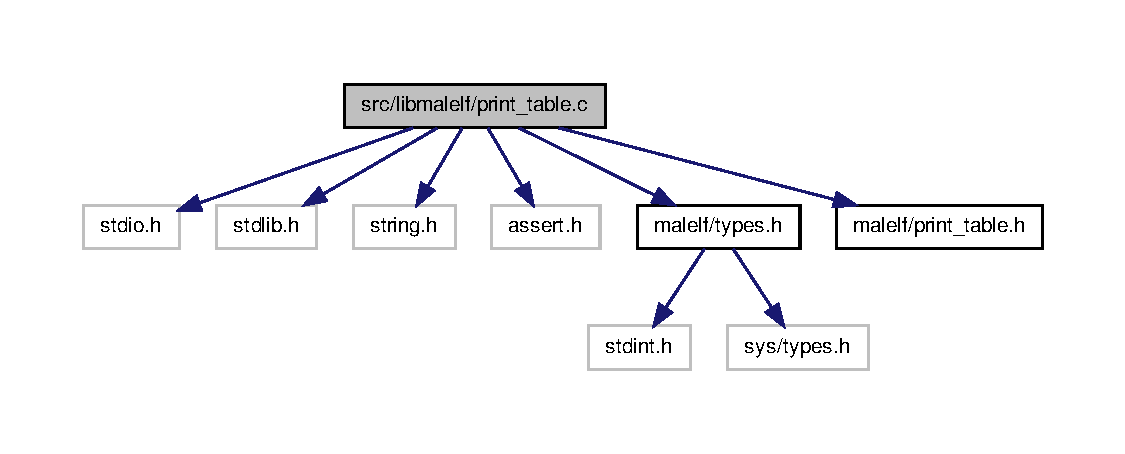
\includegraphics[width=400pt]{print__table_8c__incl}
\end{center}
\end{figure}
\subsection*{Functions}
\begin{DoxyCompactItemize}
\item 
void \hyperlink{print__table_8c_adad1379c7151cd6e882c737ad62daae9}{\_\-\_\-print\_\-table\_\-generic} (\hyperlink{structtb__line}{tb\_\-line} $\ast$l, int line\_\-size, int fit\_\-on\_\-screen, int has\_\-header)
\item 
void \hyperlink{print__table_8c_acfe0951bacb7ec31ea873aa955ee06e2}{print\_\-table\_\-header} (\hyperlink{structtb__line}{tb\_\-header} $\ast$h, int header\_\-size, int fit\_\-on\_\-screen)
\item 
void \hyperlink{print__table_8c_a9ee699b61d5f92867fbbd88dd94533c3}{print\_\-table\_\-line} (\hyperlink{structtb__line}{tb\_\-line} $\ast$l, int line\_\-size, int fit\_\-on\_\-screen)
\item 
void \hyperlink{print__table_8c_a6cecbbe406457c13d52a9ed1f35ea841}{print\_\-table\_\-header\_\-art} (int header\_\-size, int left\_\-screen)
\end{DoxyCompactItemize}
\subsection*{Variables}
\begin{DoxyCompactItemize}
\item 
\hyperlink{types_8h_af2b0f13cffd24f6dddf794ae0c7472b4}{\_\-u8} \hyperlink{print__table_8c_a9832bf9a14bd3b9656e7be172ac16c9b}{malelf\_\-quiet\_\-mode}
\begin{DoxyCompactList}\small\item\em Quiet mode. \end{DoxyCompactList}\end{DoxyCompactItemize}


\subsection{Function Documentation}
\hypertarget{print__table_8c_adad1379c7151cd6e882c737ad62daae9}{
\index{print\_\-table.c@{print\_\-table.c}!\_\-\_\-print\_\-table\_\-generic@{\_\-\_\-print\_\-table\_\-generic}}
\index{\_\-\_\-print\_\-table\_\-generic@{\_\-\_\-print\_\-table\_\-generic}!print_table.c@{print\_\-table.c}}
\subsubsection[{\_\-\_\-print\_\-table\_\-generic}]{\setlength{\rightskip}{0pt plus 5cm}void \_\-\_\-print\_\-table\_\-generic (
\begin{DoxyParamCaption}
\item[{{\bf tb\_\-line} $\ast$}]{l, }
\item[{int}]{line\_\-size, }
\item[{int}]{fit\_\-on\_\-screen, }
\item[{int}]{has\_\-header}
\end{DoxyParamCaption}
)}}
\label{print__table_8c_adad1379c7151cd6e882c737ad62daae9}
param1 = struct line param2 = size of the line table (sum of columns length) param3 = length of the screen where the table need to be positioned

This function dump a structure line or header to screen.

TODO: DANGER! THIS CODE IS UGLY AND BADLY WRITTEN!

Psychographed by i4k, written by a ghost programmer crazy!

This function was coded in early morning of 19 March, 2012. There must be hundreds of bugs but I had to write this code very fast because that the format tricks of printf doesn't help me and now I'm too lazy to improve it! All this does not justify... i know ...but I try ... 

Definition at line 31 of file print\_\-table.c.

\hypertarget{print__table_8c_acfe0951bacb7ec31ea873aa955ee06e2}{
\index{print\_\-table.c@{print\_\-table.c}!print\_\-table\_\-header@{print\_\-table\_\-header}}
\index{print\_\-table\_\-header@{print\_\-table\_\-header}!print_table.c@{print\_\-table.c}}
\subsubsection[{print\_\-table\_\-header}]{\setlength{\rightskip}{0pt plus 5cm}void print\_\-table\_\-header (
\begin{DoxyParamCaption}
\item[{{\bf tb\_\-header} $\ast$}]{h, }
\item[{int}]{header\_\-size, }
\item[{int}]{fit\_\-on\_\-screen}
\end{DoxyParamCaption}
)}}
\label{print__table_8c_acfe0951bacb7ec31ea873aa955ee06e2}


Definition at line 137 of file print\_\-table.c.

\hypertarget{print__table_8c_a6cecbbe406457c13d52a9ed1f35ea841}{
\index{print\_\-table.c@{print\_\-table.c}!print\_\-table\_\-header\_\-art@{print\_\-table\_\-header\_\-art}}
\index{print\_\-table\_\-header\_\-art@{print\_\-table\_\-header\_\-art}!print_table.c@{print\_\-table.c}}
\subsubsection[{print\_\-table\_\-header\_\-art}]{\setlength{\rightskip}{0pt plus 5cm}void print\_\-table\_\-header\_\-art (
\begin{DoxyParamCaption}
\item[{int}]{header\_\-size, }
\item[{int}]{left\_\-screen}
\end{DoxyParamCaption}
)}}
\label{print__table_8c_a6cecbbe406457c13d52a9ed1f35ea841}


Definition at line 145 of file print\_\-table.c.

\hypertarget{print__table_8c_a9ee699b61d5f92867fbbd88dd94533c3}{
\index{print\_\-table.c@{print\_\-table.c}!print\_\-table\_\-line@{print\_\-table\_\-line}}
\index{print\_\-table\_\-line@{print\_\-table\_\-line}!print_table.c@{print\_\-table.c}}
\subsubsection[{print\_\-table\_\-line}]{\setlength{\rightskip}{0pt plus 5cm}void print\_\-table\_\-line (
\begin{DoxyParamCaption}
\item[{{\bf tb\_\-line} $\ast$}]{l, }
\item[{int}]{line\_\-size, }
\item[{int}]{fit\_\-on\_\-screen}
\end{DoxyParamCaption}
)}}
\label{print__table_8c_a9ee699b61d5f92867fbbd88dd94533c3}


Definition at line 141 of file print\_\-table.c.



\subsection{Variable Documentation}
\hypertarget{print__table_8c_a9832bf9a14bd3b9656e7be172ac16c9b}{
\index{print\_\-table.c@{print\_\-table.c}!malelf\_\-quiet\_\-mode@{malelf\_\-quiet\_\-mode}}
\index{malelf\_\-quiet\_\-mode@{malelf\_\-quiet\_\-mode}!print_table.c@{print\_\-table.c}}
\subsubsection[{malelf\_\-quiet\_\-mode}]{\setlength{\rightskip}{0pt plus 5cm}{\bf \_\-u8} {\bf malelf\_\-quiet\_\-mode}}}
\label{print__table_8c_a9832bf9a14bd3b9656e7be172ac16c9b}


Quiet mode. 

get out of here immediately! cursed code!

Enable quiet mode 

Definition at line 54 of file object.c.


\hypertarget{reverse__elf_8c}{
\section{src/libmalelf/reverse\_\-elf.c File Reference}
\label{reverse__elf_8c}\index{src/libmalelf/reverse\_\-elf.c@{src/libmalelf/reverse\_\-elf.c}}
}
{\ttfamily \#include $<$stdio.h$>$}\par
{\ttfamily \#include $<$stdlib.h$>$}\par
{\ttfamily \#include $<$string.h$>$}\par
{\ttfamily \#include $<$assert.h$>$}\par
{\ttfamily \#include $<$sys/mman.h$>$}\par
{\ttfamily \#include $<$libgen.h$>$}\par
{\ttfamily \#include $<$malelf/defines.h$>$}\par
{\ttfamily \#include $<$malelf/reverse\_\-elf.h$>$}\par
{\ttfamily \#include $<$malelf/object.h$>$}\par
{\ttfamily \#include $<$malelf/types.h$>$}\par
{\ttfamily \#include $<$malelf/util.h$>$}\par
Include dependency graph for reverse\_\-elf.c:\nopagebreak
\begin{figure}[H]
\begin{center}
\leavevmode
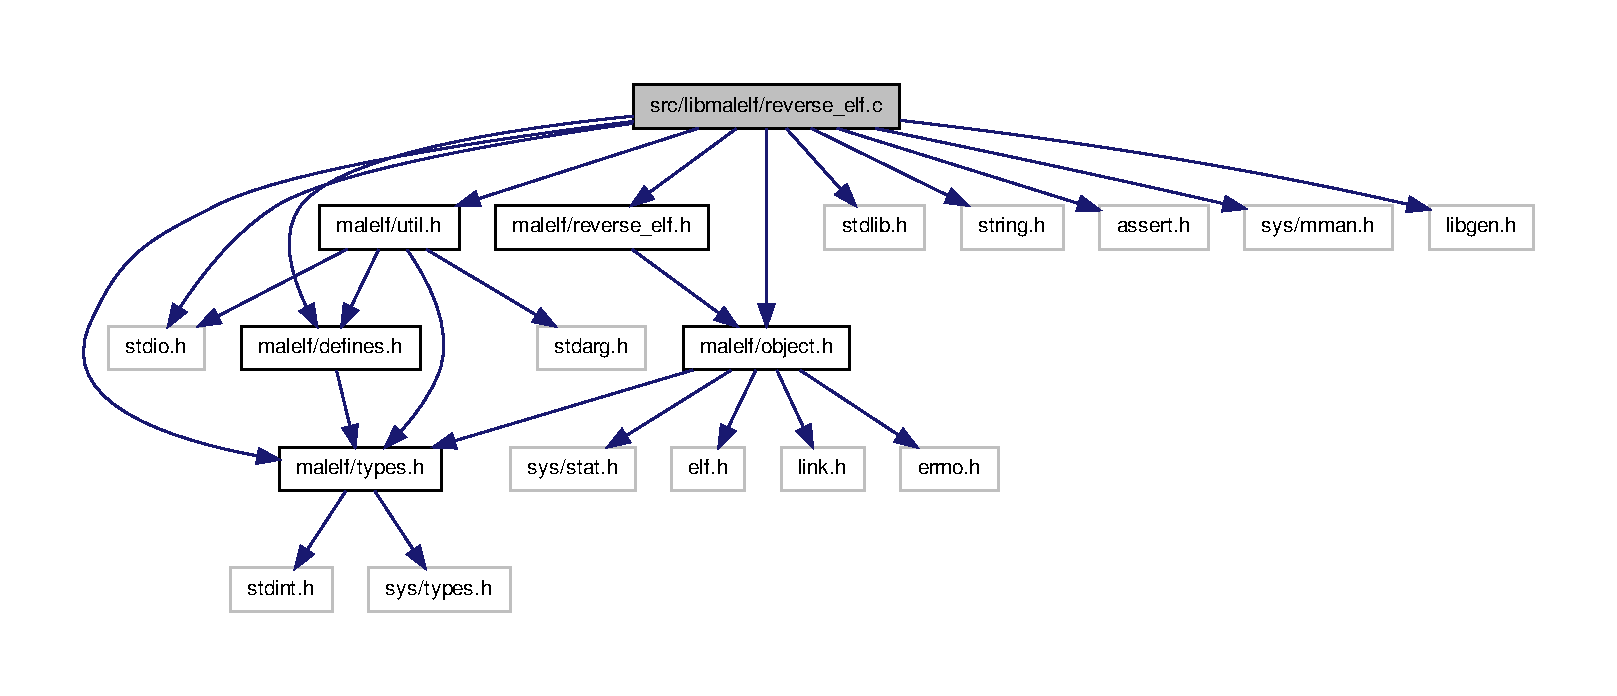
\includegraphics[width=400pt]{reverse__elf_8c__incl}
\end{center}
\end{figure}
\subsection*{Defines}
\begin{DoxyCompactItemize}
\item 
\#define \hyperlink{reverse__elf_8c_af65e1e6a295622bd6c74b699a7d83750}{TOP\_\-TEMPLATE\_\-COMMENT}~\char`\"{}$\backslash$n\char`\"{}
\item 
\#define \hyperlink{reverse__elf_8c_a06f29430a62eaea6ef6e326e5322aaa2}{TOP\_\-TEMPLATE}~TOP\_\-TEMPLATE\_\-COMMENT \char`\"{}\#include $<$stdio.h$>$$\backslash$n $\backslash$\#include $<$elf.h$>$$\backslash$n $\backslash$\#include $<$sys/types.h$>$ $\backslash$n$\backslash$\#include $<$sys/stat.h$>$$\backslash$n\#include $<$unistd.h$>$$\backslash$n$\backslash$\#include $<$fcntl.h$>$$\backslash$n$\backslash$n\char`\"{}
\item 
\#define \hyperlink{reverse__elf_8c_a6f2f6cfafaa5cc6dab98670456a034c1}{SELF\_\-GENERATE\_\-SRC}
\item 
\#define \hyperlink{reverse__elf_8c_acb0a6d3b4461a0b9a27ad3426d6de2a8}{PRINT\_\-C}~fprintf
\item 
\#define \hyperlink{reverse__elf_8c_aee4dca60970d913c2ebbcb21e89ca9b5}{PRINT\_\-FILEADDR}~PRINT\_\-C(fd, \char`\"{}/$\ast$ \%06x $\ast$/\char`\"{}, file\_\-addr);
\item 
\#define \hyperlink{reverse__elf_8c_a480b00640baf1f1902146fd554093482}{PRINT\_\-CHAR}(str, size, desc)
\item 
\#define \hyperlink{reverse__elf_8c_ad98822138b8364bf86debc9ae07cb23e}{PRINT\_\-WORD}(value, desc)~do \{ PRINT\_\-FILEADDR PRINT\_\-C(fd, \char`\"{}$\backslash$t\%d,$\backslash$t/$\ast$ \%s $\ast$/$\backslash$n\char`\"{}, value, desc); file\_\-addr += sizeof(value); \} while(0)
\item 
\#define \hyperlink{reverse__elf_8c_a2ccd27439a9345f311cf85519228dd6d}{PRINT\_\-WORD\_\-END}(value, desc)~do \{ PRINT\_\-FILEADDR PRINT\_\-C(fd, \char`\"{}$\backslash$t\%d$\backslash$t/$\ast$ \%s $\ast$/$\backslash$n\char`\"{}, value, desc); file\_\-addr += sizeof(value); \} while(0)
\item 
\#define \hyperlink{reverse__elf_8c_a69d4d1ace964579845ff71b030bb08de}{PRINT\_\-HALF}(value, desc)~PRINT\_\-WORD(value, desc)
\item 
\#define \hyperlink{reverse__elf_8c_ab07fe678941f4c46433e1786eab4709a}{PRINT\_\-ADDR}(value, desc)~do \{ PRINT\_\-FILEADDR PRINT\_\-C(fd, \char`\"{}$\backslash$t0x\%x,$\backslash$t/$\ast$ \%s $\ast$/$\backslash$n\char`\"{}, value, desc); file\_\-addr += sizeof(value); \} while(0)
\item 
\#define \hyperlink{reverse__elf_8c_a9c71bf5e7d5217429f760c271faed21d}{PRINT\_\-ADDR\_\-END}(value, desc)~do \{ PRINT\_\-FILEADDR PRINT\_\-C(fd, \char`\"{}$\backslash$t0x\%x$\backslash$t/$\ast$ \%s $\ast$/$\backslash$n\char`\"{}, value, desc); file\_\-addr += sizeof(value); \} while(0)
\item 
\#define \hyperlink{reverse__elf_8c_a6ffd8ff46a6ac94cd8c009a2faeba841}{PRINT\_\-OFF}(value, desc)~PRINT\_\-ADDR(value, desc)
\item 
\#define \hyperlink{reverse__elf_8c_ad5d1b7b30661a6996421712d8756365a}{PADCHAR}~0
\end{DoxyCompactItemize}
\subsection*{Functions}
\begin{DoxyCompactItemize}
\item 
\hyperlink{types_8h_af2b0f13cffd24f6dddf794ae0c7472b4}{\_\-u8} \hyperlink{reverse__elf_8c_af105815abb941024cdf0c799b399ff91}{reverse\_\-elf2c} (\hyperlink{structmalelf__object}{malelf\_\-object} $\ast$elf, FILE $\ast$fd)
\item 
void \hyperlink{reverse__elf_8c_ac917e62ed160fdcfb75beb21eca98f2d}{reverse\_\-elf2cgen} (int fd\_\-input, int fd\_\-output)
\end{DoxyCompactItemize}


\subsection{Define Documentation}
\hypertarget{reverse__elf_8c_ad5d1b7b30661a6996421712d8756365a}{
\index{reverse\_\-elf.c@{reverse\_\-elf.c}!PADCHAR@{PADCHAR}}
\index{PADCHAR@{PADCHAR}!reverse_elf.c@{reverse\_\-elf.c}}
\subsubsection[{PADCHAR}]{\setlength{\rightskip}{0pt plus 5cm}\#define PADCHAR~0}}
\label{reverse__elf_8c_ad5d1b7b30661a6996421712d8756365a}


Definition at line 117 of file reverse\_\-elf.c.

\hypertarget{reverse__elf_8c_ab07fe678941f4c46433e1786eab4709a}{
\index{reverse\_\-elf.c@{reverse\_\-elf.c}!PRINT\_\-ADDR@{PRINT\_\-ADDR}}
\index{PRINT\_\-ADDR@{PRINT\_\-ADDR}!reverse_elf.c@{reverse\_\-elf.c}}
\subsubsection[{PRINT\_\-ADDR}]{\setlength{\rightskip}{0pt plus 5cm}\#define PRINT\_\-ADDR(
\begin{DoxyParamCaption}
\item[{}]{value, }
\item[{}]{desc}
\end{DoxyParamCaption}
)~do \{ PRINT\_\-FILEADDR PRINT\_\-C(fd, \char`\"{}$\backslash$t0x\%x,$\backslash$t/$\ast$ \%s $\ast$/$\backslash$n\char`\"{}, value, desc); file\_\-addr += sizeof(value); \} while(0)}}
\label{reverse__elf_8c_ab07fe678941f4c46433e1786eab4709a}


Definition at line 114 of file reverse\_\-elf.c.

\hypertarget{reverse__elf_8c_a9c71bf5e7d5217429f760c271faed21d}{
\index{reverse\_\-elf.c@{reverse\_\-elf.c}!PRINT\_\-ADDR\_\-END@{PRINT\_\-ADDR\_\-END}}
\index{PRINT\_\-ADDR\_\-END@{PRINT\_\-ADDR\_\-END}!reverse_elf.c@{reverse\_\-elf.c}}
\subsubsection[{PRINT\_\-ADDR\_\-END}]{\setlength{\rightskip}{0pt plus 5cm}\#define PRINT\_\-ADDR\_\-END(
\begin{DoxyParamCaption}
\item[{}]{value, }
\item[{}]{desc}
\end{DoxyParamCaption}
)~do \{ PRINT\_\-FILEADDR PRINT\_\-C(fd, \char`\"{}$\backslash$t0x\%x$\backslash$t/$\ast$ \%s $\ast$/$\backslash$n\char`\"{}, value, desc); file\_\-addr += sizeof(value); \} while(0)}}
\label{reverse__elf_8c_a9c71bf5e7d5217429f760c271faed21d}


Definition at line 115 of file reverse\_\-elf.c.

\hypertarget{reverse__elf_8c_acb0a6d3b4461a0b9a27ad3426d6de2a8}{
\index{reverse\_\-elf.c@{reverse\_\-elf.c}!PRINT\_\-C@{PRINT\_\-C}}
\index{PRINT\_\-C@{PRINT\_\-C}!reverse_elf.c@{reverse\_\-elf.c}}
\subsubsection[{PRINT\_\-C}]{\setlength{\rightskip}{0pt plus 5cm}\#define PRINT\_\-C~fprintf}}
\label{reverse__elf_8c_acb0a6d3b4461a0b9a27ad3426d6de2a8}


Definition at line 103 of file reverse\_\-elf.c.

\hypertarget{reverse__elf_8c_a480b00640baf1f1902146fd554093482}{
\index{reverse\_\-elf.c@{reverse\_\-elf.c}!PRINT\_\-CHAR@{PRINT\_\-CHAR}}
\index{PRINT\_\-CHAR@{PRINT\_\-CHAR}!reverse_elf.c@{reverse\_\-elf.c}}
\subsubsection[{PRINT\_\-CHAR}]{\setlength{\rightskip}{0pt plus 5cm}\#define PRINT\_\-CHAR(
\begin{DoxyParamCaption}
\item[{}]{str, }
\item[{}]{size, }
\item[{}]{desc}
\end{DoxyParamCaption}
)}}
\label{reverse__elf_8c_a480b00640baf1f1902146fd554093482}
{\bfseries Value:}
\begin{DoxyCode}
do { PRINT_FILEADDR \
 PRINT_C(fd, "\t\"");                                         \
 for (_i_ = 0; _i_ < size; ++_i_) { \
   PRINT_C(fd, "\\x%x", str[_i_]); } \
 PRINT_C(fd, "\",\n"); file_addr += size; } while(0)
\end{DoxyCode}


Definition at line 105 of file reverse\_\-elf.c.

\hypertarget{reverse__elf_8c_aee4dca60970d913c2ebbcb21e89ca9b5}{
\index{reverse\_\-elf.c@{reverse\_\-elf.c}!PRINT\_\-FILEADDR@{PRINT\_\-FILEADDR}}
\index{PRINT\_\-FILEADDR@{PRINT\_\-FILEADDR}!reverse_elf.c@{reverse\_\-elf.c}}
\subsubsection[{PRINT\_\-FILEADDR}]{\setlength{\rightskip}{0pt plus 5cm}\#define PRINT\_\-FILEADDR~PRINT\_\-C(fd, \char`\"{}/$\ast$ \%06x $\ast$/\char`\"{}, file\_\-addr);}}
\label{reverse__elf_8c_aee4dca60970d913c2ebbcb21e89ca9b5}


Definition at line 104 of file reverse\_\-elf.c.

\hypertarget{reverse__elf_8c_a69d4d1ace964579845ff71b030bb08de}{
\index{reverse\_\-elf.c@{reverse\_\-elf.c}!PRINT\_\-HALF@{PRINT\_\-HALF}}
\index{PRINT\_\-HALF@{PRINT\_\-HALF}!reverse_elf.c@{reverse\_\-elf.c}}
\subsubsection[{PRINT\_\-HALF}]{\setlength{\rightskip}{0pt plus 5cm}\#define PRINT\_\-HALF(
\begin{DoxyParamCaption}
\item[{}]{value, }
\item[{}]{desc}
\end{DoxyParamCaption}
)~PRINT\_\-WORD(value, desc)}}
\label{reverse__elf_8c_a69d4d1ace964579845ff71b030bb08de}


Definition at line 113 of file reverse\_\-elf.c.

\hypertarget{reverse__elf_8c_a6ffd8ff46a6ac94cd8c009a2faeba841}{
\index{reverse\_\-elf.c@{reverse\_\-elf.c}!PRINT\_\-OFF@{PRINT\_\-OFF}}
\index{PRINT\_\-OFF@{PRINT\_\-OFF}!reverse_elf.c@{reverse\_\-elf.c}}
\subsubsection[{PRINT\_\-OFF}]{\setlength{\rightskip}{0pt plus 5cm}\#define PRINT\_\-OFF(
\begin{DoxyParamCaption}
\item[{}]{value, }
\item[{}]{desc}
\end{DoxyParamCaption}
)~PRINT\_\-ADDR(value, desc)}}
\label{reverse__elf_8c_a6ffd8ff46a6ac94cd8c009a2faeba841}


Definition at line 116 of file reverse\_\-elf.c.

\hypertarget{reverse__elf_8c_ad98822138b8364bf86debc9ae07cb23e}{
\index{reverse\_\-elf.c@{reverse\_\-elf.c}!PRINT\_\-WORD@{PRINT\_\-WORD}}
\index{PRINT\_\-WORD@{PRINT\_\-WORD}!reverse_elf.c@{reverse\_\-elf.c}}
\subsubsection[{PRINT\_\-WORD}]{\setlength{\rightskip}{0pt plus 5cm}\#define PRINT\_\-WORD(
\begin{DoxyParamCaption}
\item[{}]{value, }
\item[{}]{desc}
\end{DoxyParamCaption}
)~do \{ PRINT\_\-FILEADDR PRINT\_\-C(fd, \char`\"{}$\backslash$t\%d,$\backslash$t/$\ast$ \%s $\ast$/$\backslash$n\char`\"{}, value, desc); file\_\-addr += sizeof(value); \} while(0)}}
\label{reverse__elf_8c_ad98822138b8364bf86debc9ae07cb23e}


Definition at line 111 of file reverse\_\-elf.c.

\hypertarget{reverse__elf_8c_a2ccd27439a9345f311cf85519228dd6d}{
\index{reverse\_\-elf.c@{reverse\_\-elf.c}!PRINT\_\-WORD\_\-END@{PRINT\_\-WORD\_\-END}}
\index{PRINT\_\-WORD\_\-END@{PRINT\_\-WORD\_\-END}!reverse_elf.c@{reverse\_\-elf.c}}
\subsubsection[{PRINT\_\-WORD\_\-END}]{\setlength{\rightskip}{0pt plus 5cm}\#define PRINT\_\-WORD\_\-END(
\begin{DoxyParamCaption}
\item[{}]{value, }
\item[{}]{desc}
\end{DoxyParamCaption}
)~do \{ PRINT\_\-FILEADDR PRINT\_\-C(fd, \char`\"{}$\backslash$t\%d$\backslash$t/$\ast$ \%s $\ast$/$\backslash$n\char`\"{}, value, desc); file\_\-addr += sizeof(value); \} while(0)}}
\label{reverse__elf_8c_a2ccd27439a9345f311cf85519228dd6d}


Definition at line 112 of file reverse\_\-elf.c.

\hypertarget{reverse__elf_8c_a6f2f6cfafaa5cc6dab98670456a034c1}{
\index{reverse\_\-elf.c@{reverse\_\-elf.c}!SELF\_\-GENERATE\_\-SRC@{SELF\_\-GENERATE\_\-SRC}}
\index{SELF\_\-GENERATE\_\-SRC@{SELF\_\-GENERATE\_\-SRC}!reverse_elf.c@{reverse\_\-elf.c}}
\subsubsection[{SELF\_\-GENERATE\_\-SRC}]{\setlength{\rightskip}{0pt plus 5cm}\#define SELF\_\-GENERATE\_\-SRC}}
\label{reverse__elf_8c_a6f2f6cfafaa5cc6dab98670456a034c1}
{\bfseries Value:}
\begin{DoxyCode}
"int main() { \n" \
"    int fd; \n" \
"    fd = open(\"%s\", O_RDWR|O_CREAT); \n" \
"    if (fd == -1) { \n" \
"        perror(\"Error opening file ...\\n\"); \n" \
"        return 1; \n" \
"    } \n" \
"    if (write(fd, &elf_header, sizeof(elf_header)) != sizeof (elf_header)) { \n"
       \
"        perror(\"Error writing header to file\\n\"); \n" \
"        return 1; \n" \
"    } \n" \
"    if (write(fd, pht, sizeof(pht)) != sizeof (pht)) { \n" \
"        perror(\"Error writing pht to file\\n\"); \n" \
"        return 1; \n" \
"    } \n" \
"    if (write(fd, segments, sizeof(segments)) != sizeof(segments)) { \n" \
"        perror(\"Error writing segments to file...\\n\"); \n" \
"        return 1; \n" \
"    } \n" \
"    if (write(fd, &sht, sizeof(sht)) != sizeof(sht)) { \n" \
"        perror(\"Error writing sht to file\\n\"); \n" \
"        return 1; \n" \
"    } \n" \
"    printf(\"binary file \\\"%s\\\" successfull created.\"); \n" \
"    close(fd); \n" \
"    return 0; \n" \
"} \n"
\end{DoxyCode}


Definition at line 75 of file reverse\_\-elf.c.

\hypertarget{reverse__elf_8c_a06f29430a62eaea6ef6e326e5322aaa2}{
\index{reverse\_\-elf.c@{reverse\_\-elf.c}!TOP\_\-TEMPLATE@{TOP\_\-TEMPLATE}}
\index{TOP\_\-TEMPLATE@{TOP\_\-TEMPLATE}!reverse_elf.c@{reverse\_\-elf.c}}
\subsubsection[{TOP\_\-TEMPLATE}]{\setlength{\rightskip}{0pt plus 5cm}\#define TOP\_\-TEMPLATE~TOP\_\-TEMPLATE\_\-COMMENT \char`\"{}\#include $<$stdio.h$>$$\backslash$n $\backslash$\#include $<$elf.h$>$$\backslash$n $\backslash$\#include $<$sys/types.h$>$ $\backslash$n$\backslash$\#include $<$sys/stat.h$>$$\backslash$n\#include $<$unistd.h$>$$\backslash$n$\backslash$\#include $<$fcntl.h$>$$\backslash$n$\backslash$n\char`\"{}}}
\label{reverse__elf_8c_a06f29430a62eaea6ef6e326e5322aaa2}


Definition at line 70 of file reverse\_\-elf.c.

\hypertarget{reverse__elf_8c_af65e1e6a295622bd6c74b699a7d83750}{
\index{reverse\_\-elf.c@{reverse\_\-elf.c}!TOP\_\-TEMPLATE\_\-COMMENT@{TOP\_\-TEMPLATE\_\-COMMENT}}
\index{TOP\_\-TEMPLATE\_\-COMMENT@{TOP\_\-TEMPLATE\_\-COMMENT}!reverse_elf.c@{reverse\_\-elf.c}}
\subsubsection[{TOP\_\-TEMPLATE\_\-COMMENT}]{\setlength{\rightskip}{0pt plus 5cm}\#define TOP\_\-TEMPLATE\_\-COMMENT~\char`\"{}$\backslash$n\char`\"{}}}
\label{reverse__elf_8c_af65e1e6a295622bd6c74b699a7d83750}


Definition at line 67 of file reverse\_\-elf.c.



\subsection{Function Documentation}
\hypertarget{reverse__elf_8c_af105815abb941024cdf0c799b399ff91}{
\index{reverse\_\-elf.c@{reverse\_\-elf.c}!reverse\_\-elf2c@{reverse\_\-elf2c}}
\index{reverse\_\-elf2c@{reverse\_\-elf2c}!reverse_elf.c@{reverse\_\-elf.c}}
\subsubsection[{reverse\_\-elf2c}]{\setlength{\rightskip}{0pt plus 5cm}{\bf \_\-u8} reverse\_\-elf2c (
\begin{DoxyParamCaption}
\item[{{\bf malelf\_\-object} $\ast$}]{elf, }
\item[{FILE $\ast$}]{fd}
\end{DoxyParamCaption}
)}}
\label{reverse__elf_8c_af105815abb941024cdf0c799b399ff91}


Definition at line 120 of file reverse\_\-elf.c.

\hypertarget{reverse__elf_8c_ac917e62ed160fdcfb75beb21eca98f2d}{
\index{reverse\_\-elf.c@{reverse\_\-elf.c}!reverse\_\-elf2cgen@{reverse\_\-elf2cgen}}
\index{reverse\_\-elf2cgen@{reverse\_\-elf2cgen}!reverse_elf.c@{reverse\_\-elf.c}}
\subsubsection[{reverse\_\-elf2cgen}]{\setlength{\rightskip}{0pt plus 5cm}void reverse\_\-elf2cgen (
\begin{DoxyParamCaption}
\item[{int}]{fd\_\-input, }
\item[{int}]{fd\_\-output}
\end{DoxyParamCaption}
)}}
\label{reverse__elf_8c_ac917e62ed160fdcfb75beb21eca98f2d}


Definition at line 307 of file reverse\_\-elf.c.


\hypertarget{section__types_8inc}{
\section{src/libmalelf/section\_\-types.inc File Reference}
\label{section__types_8inc}\index{src/libmalelf/section\_\-types.inc@{src/libmalelf/section\_\-types.inc}}
}
This graph shows which files directly or indirectly include this file:\nopagebreak
\begin{figure}[H]
\begin{center}
\leavevmode
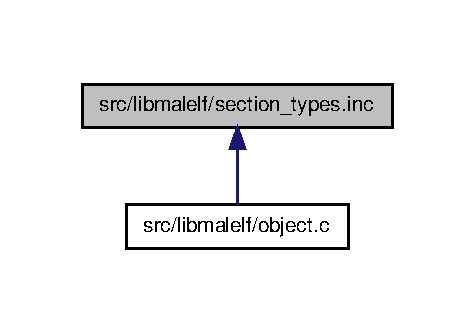
\includegraphics[width=228pt]{section__types_8inc__dep__incl}
\end{center}
\end{figure}

\hypertarget{segment__flags_8inc}{
\section{src/libmalelf/segment\_\-flags.inc File Reference}
\label{segment__flags_8inc}\index{src/libmalelf/segment\_\-flags.inc@{src/libmalelf/segment\_\-flags.inc}}
}
This graph shows which files directly or indirectly include this file:\nopagebreak
\begin{figure}[H]
\begin{center}
\leavevmode
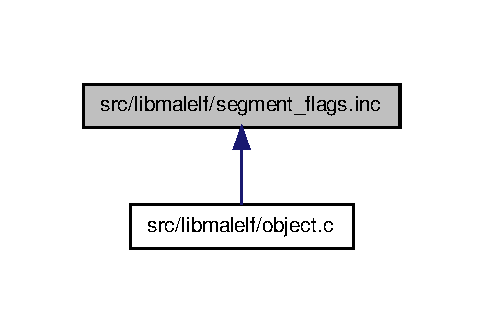
\includegraphics[width=232pt]{segment__flags_8inc__dep__incl}
\end{center}
\end{figure}

\hypertarget{segment__types_8inc}{
\section{src/libmalelf/segment\_\-types.inc File Reference}
\label{segment__types_8inc}\index{src/libmalelf/segment\_\-types.inc@{src/libmalelf/segment\_\-types.inc}}
}
This graph shows which files directly or indirectly include this file:\nopagebreak
\begin{figure}[H]
\begin{center}
\leavevmode
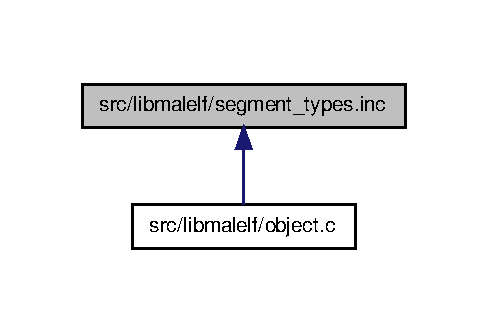
\includegraphics[width=234pt]{segment__types_8inc__dep__incl}
\end{center}
\end{figure}

\hypertarget{shellcode_8c}{
\section{src/libmalelf/shellcode.c File Reference}
\label{shellcode_8c}\index{src/libmalelf/shellcode.c@{src/libmalelf/shellcode.c}}
}
{\ttfamily \#include $<$stdio.h$>$}\par
{\ttfamily \#include $<$stdlib.h$>$}\par
{\ttfamily \#include $<$sys/mman.h$>$}\par
{\ttfamily \#include $<$malelf/object.h$>$}\par
{\ttfamily \#include $<$malelf/defines.h$>$}\par
{\ttfamily \#include $<$malelf/util.h$>$}\par
{\ttfamily \#include $<$malelf/error.h$>$}\par
{\ttfamily \#include $<$malelf/types.h$>$}\par
{\ttfamily \#include $<$malelf/infect.h$>$}\par
Include dependency graph for shellcode.c:\nopagebreak
\begin{figure}[H]
\begin{center}
\leavevmode
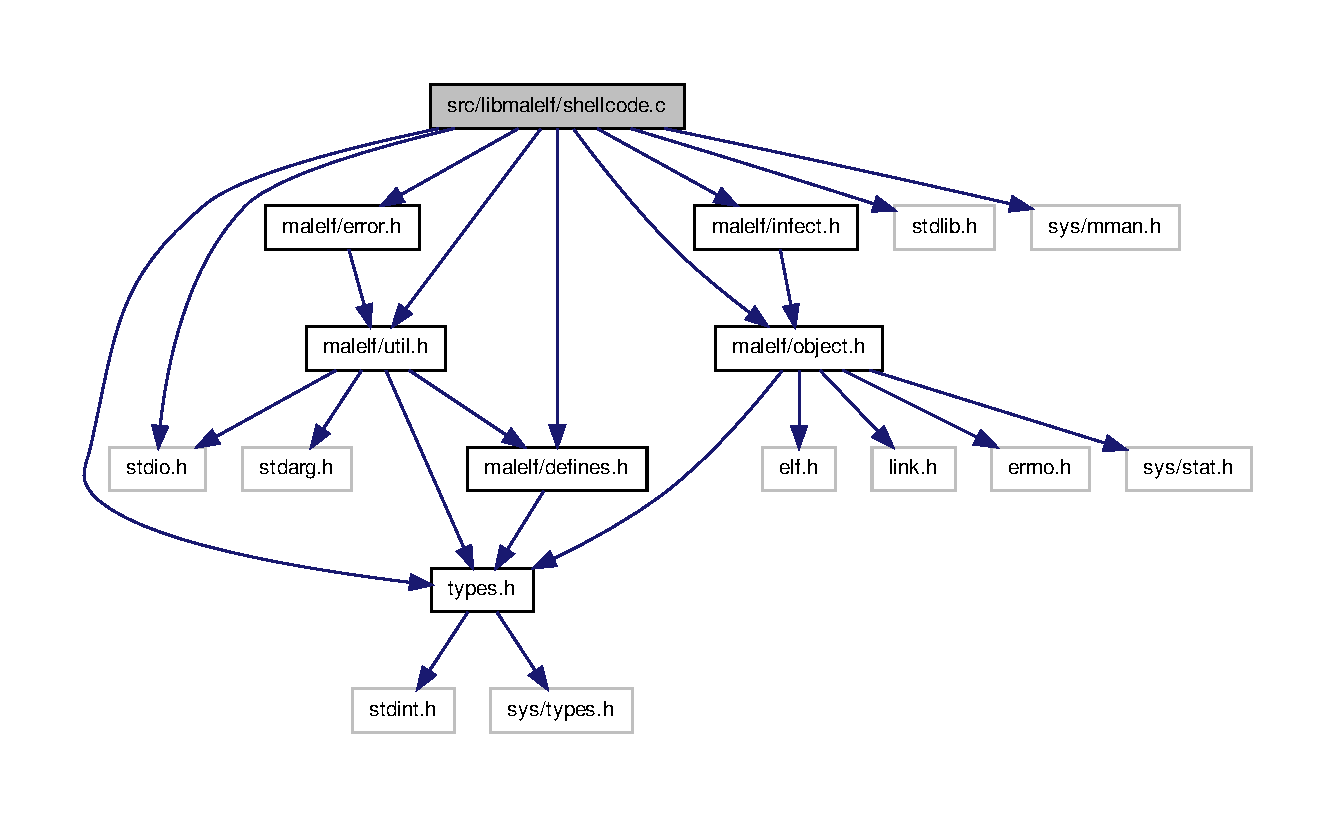
\includegraphics[width=400pt]{shellcode_8c__incl}
\end{center}
\end{figure}
\subsection*{Functions}
\begin{DoxyCompactItemize}
\item 
\hyperlink{types_8h_aacb1ea6e27efde1c708a8bc4b56ee1a2}{\_\-i32} \hyperlink{shellcode_8c_ae48b8cf662162251fb5f2acc23135295}{shellcode\_\-create\_\-malelficus} (FILE $\ast$fd\_\-o, int in\_\-size, FILE $\ast$fd\_\-i, unsigned long int original\_\-entry\_\-point, unsigned long int magic\_\-bytes)
\item 
\hyperlink{types_8h_af2b0f13cffd24f6dddf794ae0c7472b4}{\_\-u8} \hyperlink{shellcode_8c_af8c79b848eff9ca4ea257b7de598cc4c}{shellcode\_\-create\_\-c} (FILE $\ast$fd\_\-o, int in\_\-size, FILE $\ast$fd\_\-i, unsigned long int original\_\-entry\_\-point)
\end{DoxyCompactItemize}


\subsection{Function Documentation}
\hypertarget{shellcode_8c_af8c79b848eff9ca4ea257b7de598cc4c}{
\index{shellcode.c@{shellcode.c}!shellcode\_\-create\_\-c@{shellcode\_\-create\_\-c}}
\index{shellcode\_\-create\_\-c@{shellcode\_\-create\_\-c}!shellcode.c@{shellcode.c}}
\subsubsection[{shellcode\_\-create\_\-c}]{\setlength{\rightskip}{0pt plus 5cm}{\bf \_\-u8} shellcode\_\-create\_\-c (
\begin{DoxyParamCaption}
\item[{FILE $\ast$}]{fd\_\-o, }
\item[{int}]{in\_\-size, }
\item[{FILE $\ast$}]{fd\_\-i, }
\item[{unsigned long int}]{original\_\-entry\_\-point}
\end{DoxyParamCaption}
)}}
\label{shellcode_8c_af8c79b848eff9ca4ea257b7de598cc4c}


Definition at line 59 of file shellcode.c.

\hypertarget{shellcode_8c_ae48b8cf662162251fb5f2acc23135295}{
\index{shellcode.c@{shellcode.c}!shellcode\_\-create\_\-malelficus@{shellcode\_\-create\_\-malelficus}}
\index{shellcode\_\-create\_\-malelficus@{shellcode\_\-create\_\-malelficus}!shellcode.c@{shellcode.c}}
\subsubsection[{shellcode\_\-create\_\-malelficus}]{\setlength{\rightskip}{0pt plus 5cm}{\bf \_\-i32} shellcode\_\-create\_\-malelficus (
\begin{DoxyParamCaption}
\item[{FILE $\ast$}]{fd\_\-o, }
\item[{int}]{in\_\-size, }
\item[{FILE $\ast$}]{fd\_\-i, }
\item[{unsigned long int}]{original\_\-entry\_\-point, }
\item[{unsigned long int}]{magic\_\-bytes}
\end{DoxyParamCaption}
)}}
\label{shellcode_8c_ae48b8cf662162251fb5f2acc23135295}


Definition at line 16 of file shellcode.c.


\hypertarget{util_8c}{
\section{src/libmalelf/util.c File Reference}
\label{util_8c}\index{src/libmalelf/util.c@{src/libmalelf/util.c}}
}
{\ttfamily \#include $<$stdio.h$>$}\par
{\ttfamily \#include $<$stdlib.h$>$}\par
{\ttfamily \#include $<$string.h$>$}\par
{\ttfamily \#include $<$strings.h$>$}\par
{\ttfamily \#include $<$stdarg.h$>$}\par
{\ttfamily \#include $<$sys/stat.h$>$}\par
{\ttfamily \#include $<$fcntl.h$>$}\par
{\ttfamily \#include $<$unistd.h$>$}\par
{\ttfamily \#include $<$malelf/util.h$>$}\par
{\ttfamily \#include $<$malelf/error.h$>$}\par
Include dependency graph for util.c:\nopagebreak
\begin{figure}[H]
\begin{center}
\leavevmode
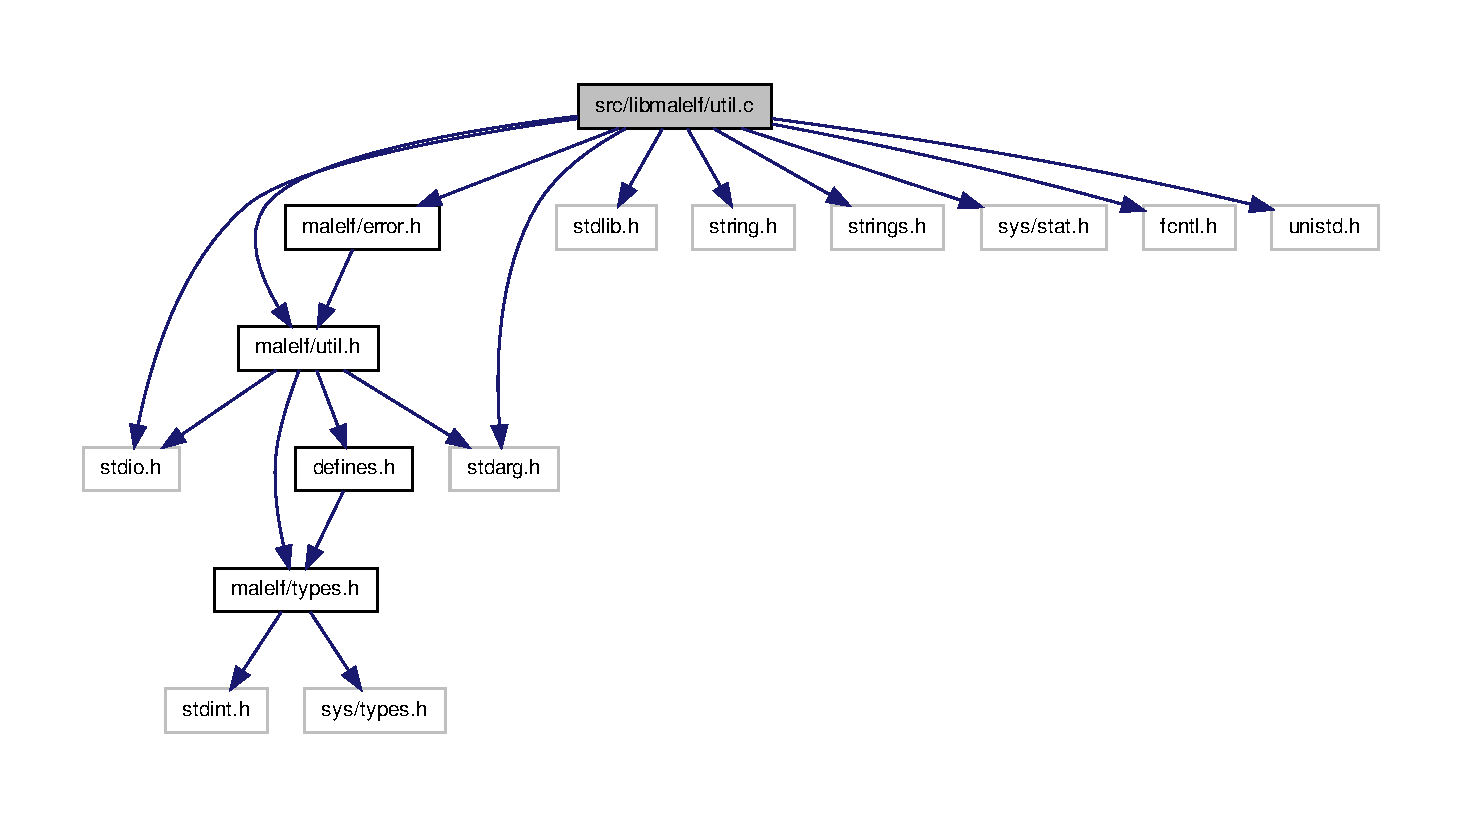
\includegraphics[width=400pt]{util_8c__incl}
\end{center}
\end{figure}
\subsection*{Functions}
\begin{DoxyCompactItemize}
\item 
int \hyperlink{util_8c_a247542ae0b6acc9ada0109283141c737}{malelf\_\-log} (FILE $\ast$fd, const char $\ast$prefix, const char $\ast$format, va\_\-list args)
\item 
int \hyperlink{util_8c_ac6734a7443633a78f6a87d5511ca2364}{malelf\_\-print} (FILE $\ast$fd, const char $\ast$format,...)
\item 
int \hyperlink{util_8c_a1cd6a5086679cbb2b107e781aeb3835d}{malelf\_\-say} (const char $\ast$format,...)
\item 
int \hyperlink{util_8c_a9d6a039b287860279870f4297d80ef6a}{malelf\_\-error} (const char $\ast$format,...)
\item 
int \hyperlink{util_8c_aea4d2b93d2acad2b43abc0aff8680828}{malelf\_\-success} (const char $\ast$format,...)
\item 
int \hyperlink{util_8c_abf9a0a02da3599092c0aa5cbbe62ff2f}{malelf\_\-warn} (const char $\ast$format,...)
\item 
\hyperlink{types_8h_af2b0f13cffd24f6dddf794ae0c7472b4}{\_\-u8} \hyperlink{util_8c_a7030062f94da236e11cadbd65d7a2c29}{saveFile} (const char $\ast$fname, \hyperlink{types_8h_af2b0f13cffd24f6dddf794ae0c7472b4}{\_\-u8} $\ast$mem, off\_\-t size)
\end{DoxyCompactItemize}
\subsection*{Variables}
\begin{DoxyCompactItemize}
\item 
\hyperlink{types_8h_af2b0f13cffd24f6dddf794ae0c7472b4}{\_\-u8} \hyperlink{util_8c_a9832bf9a14bd3b9656e7be172ac16c9b}{malelf\_\-quiet\_\-mode}
\begin{DoxyCompactList}\small\item\em Quiet mode. \end{DoxyCompactList}\end{DoxyCompactItemize}


\subsection{Function Documentation}
\hypertarget{util_8c_a9d6a039b287860279870f4297d80ef6a}{
\index{util.c@{util.c}!malelf\_\-error@{malelf\_\-error}}
\index{malelf\_\-error@{malelf\_\-error}!util.c@{util.c}}
\subsubsection[{malelf\_\-error}]{\setlength{\rightskip}{0pt plus 5cm}int malelf\_\-error (
\begin{DoxyParamCaption}
\item[{const char $\ast$}]{format, }
\item[{}]{...}
\end{DoxyParamCaption}
)}}
\label{util_8c_a9d6a039b287860279870f4297d80ef6a}


Definition at line 49 of file util.c.

\hypertarget{util_8c_a247542ae0b6acc9ada0109283141c737}{
\index{util.c@{util.c}!malelf\_\-log@{malelf\_\-log}}
\index{malelf\_\-log@{malelf\_\-log}!util.c@{util.c}}
\subsubsection[{malelf\_\-log}]{\setlength{\rightskip}{0pt plus 5cm}int malelf\_\-log (
\begin{DoxyParamCaption}
\item[{FILE $\ast$}]{fd, }
\item[{const char $\ast$}]{prefix, }
\item[{const char $\ast$}]{format, }
\item[{va\_\-list}]{args}
\end{DoxyParamCaption}
)}}
\label{util_8c_a247542ae0b6acc9ada0109283141c737}


Definition at line 15 of file util.c.

\hypertarget{util_8c_ac6734a7443633a78f6a87d5511ca2364}{
\index{util.c@{util.c}!malelf\_\-print@{malelf\_\-print}}
\index{malelf\_\-print@{malelf\_\-print}!util.c@{util.c}}
\subsubsection[{malelf\_\-print}]{\setlength{\rightskip}{0pt plus 5cm}int malelf\_\-print (
\begin{DoxyParamCaption}
\item[{FILE $\ast$}]{fd, }
\item[{const char $\ast$}]{format, }
\item[{}]{...}
\end{DoxyParamCaption}
)}}
\label{util_8c_ac6734a7443633a78f6a87d5511ca2364}


Definition at line 37 of file util.c.

\hypertarget{util_8c_a1cd6a5086679cbb2b107e781aeb3835d}{
\index{util.c@{util.c}!malelf\_\-say@{malelf\_\-say}}
\index{malelf\_\-say@{malelf\_\-say}!util.c@{util.c}}
\subsubsection[{malelf\_\-say}]{\setlength{\rightskip}{0pt plus 5cm}int malelf\_\-say (
\begin{DoxyParamCaption}
\item[{const char $\ast$}]{format, }
\item[{}]{...}
\end{DoxyParamCaption}
)}}
\label{util_8c_a1cd6a5086679cbb2b107e781aeb3835d}


Definition at line 43 of file util.c.

\hypertarget{util_8c_aea4d2b93d2acad2b43abc0aff8680828}{
\index{util.c@{util.c}!malelf\_\-success@{malelf\_\-success}}
\index{malelf\_\-success@{malelf\_\-success}!util.c@{util.c}}
\subsubsection[{malelf\_\-success}]{\setlength{\rightskip}{0pt plus 5cm}int malelf\_\-success (
\begin{DoxyParamCaption}
\item[{const char $\ast$}]{format, }
\item[{}]{...}
\end{DoxyParamCaption}
)}}
\label{util_8c_aea4d2b93d2acad2b43abc0aff8680828}


Definition at line 55 of file util.c.

\hypertarget{util_8c_abf9a0a02da3599092c0aa5cbbe62ff2f}{
\index{util.c@{util.c}!malelf\_\-warn@{malelf\_\-warn}}
\index{malelf\_\-warn@{malelf\_\-warn}!util.c@{util.c}}
\subsubsection[{malelf\_\-warn}]{\setlength{\rightskip}{0pt plus 5cm}int malelf\_\-warn (
\begin{DoxyParamCaption}
\item[{const char $\ast$}]{format, }
\item[{}]{...}
\end{DoxyParamCaption}
)}}
\label{util_8c_abf9a0a02da3599092c0aa5cbbe62ff2f}


Definition at line 61 of file util.c.

\hypertarget{util_8c_a7030062f94da236e11cadbd65d7a2c29}{
\index{util.c@{util.c}!saveFile@{saveFile}}
\index{saveFile@{saveFile}!util.c@{util.c}}
\subsubsection[{saveFile}]{\setlength{\rightskip}{0pt plus 5cm}{\bf \_\-u8} saveFile (
\begin{DoxyParamCaption}
\item[{const char $\ast$}]{fname, }
\item[{{\bf \_\-u8} $\ast$}]{mem, }
\item[{off\_\-t}]{size}
\end{DoxyParamCaption}
)}}
\label{util_8c_a7030062f94da236e11cadbd65d7a2c29}


Definition at line 67 of file util.c.



\subsection{Variable Documentation}
\hypertarget{util_8c_a9832bf9a14bd3b9656e7be172ac16c9b}{
\index{util.c@{util.c}!malelf\_\-quiet\_\-mode@{malelf\_\-quiet\_\-mode}}
\index{malelf\_\-quiet\_\-mode@{malelf\_\-quiet\_\-mode}!util.c@{util.c}}
\subsubsection[{malelf\_\-quiet\_\-mode}]{\setlength{\rightskip}{0pt plus 5cm}{\bf \_\-u8} {\bf malelf\_\-quiet\_\-mode}}}
\label{util_8c_a9832bf9a14bd3b9656e7be172ac16c9b}


Quiet mode. 

Enable quiet mode 

Definition at line 54 of file object.c.


\printindex
\end{document}
